%!TEX program = xelatex
% arara: xelatex
% Author: Alfredo Sánchez Alberca (asalber@gmail.com)
% ASPECT RATIO FOR YOUTUBE VIDEO
% \documentclass[aspectratio=1610,mathserif,profesionalfont,10pt,svgnames,red,xcolor=table]{beamer}
% ASPECT RATIO FOR PROJECTOR
%\documentclass[profesionalfont,10pt,svgnames,xcolor=table]{beamer}

% BEAMER THEME
%\usetheme[progressbar=frametitle,background=light,titleformat=smallcaps,block=fill]{metropolis}

% ARTICLE VERSION
% \pdfminorversion=4 % for solving some problems with png graphics in acrobat reader
\documentclass[10pt,a4paper,titlepage]{article}
\usepackage[hyperref]{beamerarticle}

\usepackage{standalone}

% LANGUAGE
\usepackage{polyglossia}
\setdefaultlanguage{english}

% FONT
%\usefonttheme{professionalfonts}
%\usepackage{cmbright}
%\setmainfont{CMU Bright}
%\setmathfont{Arial}
 

\mode<article>{
\usepackage{fontspec}
\usepackage{unicode-math}
\setmainfont[Ligatures=TeX]{TeX Gyre Pagella}
\setmathfont[math-style=ISO,bold-style=ISO,vargreek-shape=TeX]{TeX Gyre Pagella Math}
%\usepackage[sc]{mathpazo}
%\setromanfont[Mapping=tex-text]{Linux Libertine}
%\setsansfont[Mapping=tex-text]{Myriad Pro}
%\setmonofont[Mapping=tex-text]{Courier New}
}
% IMPROVE FONT IN PDF
\mode<article>{\usepackage{microtype}}

% MATHS
\usepackage{amsmath}
\usepackage{units}

% MARGINS
\setbeamersize{text margin left=.5cm, text margin right=.5cm}

% MARGINS FOR ARTICLE
\mode<article>{\usepackage{fullpage}}
\mode<article>{\usepackage[headsep=1cm, top=3cm, bottom=3cm, left=2.54cm, right=2.54cm]{geometry}}

% COLORS
% Author: Alfredo Sánchez Alberca (asalber@ceu.es)
\usepackage{xcolor}
\definecolor{color1}{RGB}{5,161,230} % Blue
\definecolor{color2}{RGB}{238,50,36} % Red
\definecolor{color3}{RGB}{0,205,0} % Green
\definecolor{color4}{RGB}{243,102,25} % Orange
\definecolor{ocre}{RGB}{243,102,25} % Define the orange color used for highlighting throughout the book
\definecolor{blueceu}{RGB}{5,161,230} % Blue color of CEU logo
\definecolor{greenceu}{RGB}{185,209,16} % Green color of CEU logo
\definecolor{redceu}{RGB}{238,50,36} % Red color of CEU logo
\definecolor{grayceu}{RGB}{111,107,83} % Gray color of CEU logo
\definecolor{coral}{rgb}{1,0.5,0.31} % Orange color for graphics
\definecolor{royalblue1}{rgb}{0.28,0.46,1} % Blue color for graphics
\definecolor{mygreen}{rgb}{0,0.8,0} % Green color for graphics
\definecolor{chaptergrey}{RGB}{5,161,230} % Blue color of CEU logo
\definecolor{DarkBrown}{HTML}{604c38} % Brown of Metropoly theme
\definecolor{DarkTeal}{HTML}{23373b} % Teal of Metropoly theme

% TABLE OF CONTENT style
\setbeamertemplate{section in toc}[sections numbered]
\setbeamertemplate{subsection in toc}[subsections numbered]

% TABLES
\usepackage{array}
\usepackage{multirow}
\usepackage{colortbl}
\usepackage{booktabs}
\newcommand{\tcrule}{\arrayrulecolor{color1!50!white}\toprule}
\newcommand{\mcrule}{\arrayrulecolor{color1!50!white}\midrule}
\newcommand{\bcrule}{\arrayrulecolor{color1!50!white}\bottomrule}

\listfiles
% GRAPHICS
\usepackage{pgfplots}
\usepgfplotslibrary{fillbetween}
% pgfplots styles
% Author: Alfredo Sánchez Alberca (asalber@ceu.es)

\pgfplotsset{colormap={outcolormap}{color=(color1); color=(color1!50)},
             colormap={incolormap}{color=(color2); color=(color2!50)},
             colormap={twocolormap}{color=(color1); color=(color2)}}

% Line styles for plotting 2d functions
\pgfplotscreateplotcyclelist{2dfun cycle}{%
  {color1, line width=0.8pt},
  {color2, line width=0.8pt},
  {color3, line width=0.8pt},
  {color4, line width=0.8pt},
}
% Line and point styles for plotting 2d data
\pgfplotscreateplotcyclelist{2dplot cycle}{%
  {color1, line width=0.8pt, mark=*, mark size=1.5pt},
  {color2, line width=0.8pt, mark=square*, mark size=1.3pt},
  {color3, line width=0.8pt, mark=triangle*, mark size=1.5pt},
  {color4, line width=0.8pt, mark=diamond*, mark size=1.5pt},
}

% Plot styles
\pgfplotsset{
  compat=1.14,
% Basic 2D settings
  2dbaseplot/.style={
    axis line style={<->}, % arrows on the axis
    scale only axis,        % otherwise width won't be as intended: http://tex.stackexchange.com/questions/36297/pgfplots-how-can-i-scale-to-text-width
    x tick label style={font=\small},
    y tick label style={font=\small},
    every axis/.append style={font=\small}, 
  },
% Settings for generic 2D functions 
  gen2dfun/.style={
    2dbaseplot,
    axis x line=middle,
    axis y line=middle,
    xlabel={$x$},         
    ylabel={$y$},          
    every axis x label/.style={at={(ticklabel* cs:1)}, anchor=west,},
	every axis y label/.style={at={(ticklabel* cs:1)}, anchor=south,},
    cycle list name=2dfun cycle,
  },
% Settings for 2D functions 
  2dfun/.style={
    2dbaseplot,
    axis x line=middle,
    axis y line=middle,
    xlabel={$x$},         
    ylabel={$y$},          
    every axis x label/.style={at={(ticklabel* cs:1)}, anchor=west,},
	every axis y label/.style={at={(ticklabel* cs:1)}, anchor=south,},
    x tick label style={font=\tiny},
    y tick label style={font=\tiny},
    cycle list name=2dfun cycle,
  },
% Settings for 2D plots
  2dplot/.style={
    baseplot,
    xmajorgrids=true,
    ymajorgrids=true,
    major grid style={dotted},
    axis x line=bottom,
    axis y line=left,
    legend style={cells={anchor=west}, draw=none, font=\footnotesize},
    x tick label style={font=\tiny}, 
    y tick label style={font=\tiny},
    cycle list name=2dplot cycle,
  },
% Basic 3D settings
  3dbaseplot/.style={
%    axis line style={->}, % arrows on the axis
    scale only axis,        % otherwise width won't be as intended: http://tex.stackexchange.com/questions/36297/pgfplots-how-can-i-scale-to-text-width
    x tick label style={font=\small},
    y tick label style={font=\small},
    z tick label style={font=\small},
    every axis/.append style={font=\small}, 
  },
% Settings for generic 3D functions 
  gen3dfun/.style={
    3dbaseplot,
    xlabel={$x$},         
    ylabel={$y$},
    zlabel={$z$},
    every axis x label/.style={at={(ticklabel cs:0.5)}, anchor=center,},
	every axis y label/.style={at={(ticklabel cs:0.5)}, anchor=center,},
	every axis z label/.style={at={(ticklabel cs:0.5)}, anchor=center,},           
    cycle list name=2dfun cycle,
  },
% Settings for 3D functions 
  3dfun/.style={
    3dbaseplot,
    xlabel={$x$},         
    ylabel={$y$},
    zlabel={$z$},           
    every axis x label/.style={at={(ticklabel cs:0.5)}, anchor=center,},
	every axis y label/.style={at={(ticklabel cs:0.5)}, anchor=center,},
	every axis z label/.style={at={(ticklabel cs:0.5)}, anchor=center,},
	x tick label style={font=\tiny}, 
    y tick label style={font=\tiny},
    z tick label style={font=\tiny},
    cycle list name=2dfun cycle,
  },
}

\usepackage{tikz}
\usetikzlibrary{external, arrows, arrows.meta, calc, shapes, shapes.arrows, positioning, decorations.pathreplacing, intersections}
% TIKZ SETTINGS
\tikzset{
	% Overlays
    invisible/.style={opacity=0},
    visible on/.style={alt={#1{}{invisible}}},
    alt/.code args={<#1>#2#3}{%
      \alt<#1>{\pgfkeysalso{#2}}{\pgfkeysalso{#3}} % \pgfkeysalso doesn't change the path
    },
    % Vectors
    vector/.style={->, color1, thick},
    % Arrow tips
    >=stealth,
  }
% \usepackage{tkz-euclide}
% \usetkzobj{all}
% Graphics export
\mode<article>{
\tikzset{
    png export/.style={
        external/system call={
            xelatex \tikzexternalcheckshellescape -halt-on-error -interaction=batchmode -jobname "\image" "\texsource";
            convert -density 300 -transparent white "\image.pdf" "\image.png"
        }
    }
}
\tikzset{
	svg export/.style={
        external/system call/.add={}%
        {; pdf2svg "\image.pdf" "\image.svg"}
    }
}
\tikzexternalize[prefix=img/exported/]
\tikzset{png export}
\tikzset{svg export}
}

\usepackage{graphicx}

% CREATIVE COMMON ICONS
\usepackage[scale=2]{ccicons}

% LOGO POSITION
\setbeamertemplate{title graphic}{
 \vbox to 0pt {
 	\vspace*{0.9\textheight}
 	\inserttitlegraphic
 }
}

% SPACE BETWEEN PARAGRAFS
\setlength{\parskip}{0.5em}

% THEORMEM ENVIRONMENTS
%\theoremstyle{definition}
%\newtheorem{defin}[theorem]{Definition}

% BLOCKS COLORS
\setbeamercolor{block title}{
	use=normal text,
	fg=normal text.fg,
	bg=alerted text.fg!50
}

% OPERATORS
\newcommand{\dom}{{\operatorname{Dom}}}


% HEADINGS AND FOOTERS FOR ARTICLE
\mode<article>{
\usepackage{fancyhdr}
\pagestyle{fancy}
\rhead{\sffamily\slshape Elementary Calculus Manual}
\renewcommand{\headrulewidth}{0pt}
%\renewcommand{\floatpagefraction}{.8}
%\renewcommand{\textfraction}{.1}
}

% FRAME TITLE CONFIGURATION
% \defbeamertemplate{frametitle}{myframe}{
% 	\nointerlineskip
% 	\begin{beamercolorbox}[wd=\paperwidth,sep=1ex]{frametitle}
% 		\insertframetitle
% 	\end{beamercolorbox}
% }
% \setbeamertemplate{frametitle}[myframe]

% SECTION COLOR FOR ARTICLE
\mode<article>{
\usepackage{titlesec}
\titleformat{\section}{\color{color1}\normalfont\Large\bfseries}{\color{color1}\thesection}{1em}{}
\titleformat{\subsection}{\color{color1}\normalfont\large\bfseries}{\color{color1}\thesubsection}{1em}{}
}

% COMMAND FOR HIGHLIGHTING
\newcommand{\highlight}[1]{\textcolor{orange}{\textbf{#1}}}

% PDF settings
\hypersetup{colorlinks=true}

%=====================================================================BODY=====

%---------------------------------------------------------------------cover----
\mode<article>{
\title{\textcolor{color1}{\Huge Elementary Calculus Manual}}
\author{
Santiago Angulo Díaz-Parreño (\href{mailto:sangulo@ceu.es}{sangulo@ceu.es}) &
Pablo Ares Gastesi (\href{mailto:pablo.aresgastesi@ceu.es}{pablo.aresgastesi@ceu.es}) &
José Rojo Montijano (\href{mailto:jrojo.eps@ceu.es}{jrojo.eps@ceu.es}) &
Anselmo Romero Limón (\href{mailto:arlimon@ceu.es}{arlimon@ceu.es}) &
Alfredo Sánchez Alberca (\href{mailto:asalber@ceu.es}{asalber@ceu.es})
}
\date{Sep 2016\\[1cm]
Department of Applied Math and Statistics\\ CEU San Pablo\\[1cm]

\includegraphics[height=2cm]{img/logo_uspceu}
}
}
\mode<presentation>{
\title{Elementary Calculus Manual}
\author{
Alfredo Sánchez Alberca (\href{mailto:asalber@ceu.es}{asalber@ceu.es})}
\institute{Department of Applied Math and Statistics\\ CEU San Pablo}
\date{Sep 2016}
\titlegraphic{\hfill
\includegraphics[height=1.5cm]{img/logo_uspceu}}
}



\begin{document}
\mode<article>{\thispagestyle{empty}\maketitle}
\mode<presentation>{\maketitle}

%---------------------------------------------------------------------slide----
\begin{frame}
% Creative Commons 2.5 license terms
\frametitle{License terms \normalsize \ccLogo}

\scriptsize
This work is licensed under an Attribution-NonCommercial-ShareAlike 4.0 International Creative Commons License. 
\url{http://creativecommons.org/licenses/by-nc-sa/4.0/}

You are free to: 

\begin{itemize}
\item Share -- copy and redistribute the material in any medium or format
\item Adapt -- remix, transform, and build upon the material
\end{itemize}

Under the following terms:
\begin{center}
\begin{tabular}{cp{0.8\textwidth}}
\ccAttribution &  \textbf{Attribution}. You must give appropriate credit, provide a link
to the license, and indicate if changes were made. You may do so in any reasonable manner, but not in any way that
suggests the licensor endorses you or your use.\\ 
\ccNonCommercialEU & \textbf{NonComercial}. You may not use the material for commercial purposes.\\ 
\ccShareAlike & \textbf{ShareAlike}. If you remix, transform, or build upon the material, you must distribute
your contributions under the same license as the original.
\end{tabular}
\end{center}

No additional restrictions — You may not apply legal terms or technological measures that legally restrict others from
doing anything the license permits.

\end{frame}

\mode<article>{\clearpage}

%---------------------------------------------------------------------slide----
\begin{frame}
\mode<presentation>{\frametitle{Contents}}
\setbeamertemplate{section in toc}[sections numbered]
\tableofcontents[hideallsubsections]
\end{frame}

% Author: Alfredo Sánchez Alberca (asalber@ceu.es)
\section{Analytic geometry}

%---------------------------------------------------------------------slide----
\begin{frame}
\frametitle{Analytic geometry}
\setlength{\parskip}{0.3em}
\tableofcontents[sectionstyle=show/hide,hideothersubsections]
\end{frame}

\subsection{Vectors}

%---------------------------------------------------------------------slide----
\begin{frame}
\frametitle{Scalars}
Some phenomena of Nature can be described by a number and a unit of measurement. 

\begin{definition}[Scalar]
A \emph{scalar} is a number that expresses a magnitude without direction.
\end{definition}
\structure{\bfseries Examples} The height or weight of a person, the temperature of a gas or the time it takes a vehicle to travel a distance.

However, there are other phenomena that cannot be described adequately by a scalar. 
If, for instance, a sailor wants to head for seaport and only knows the intensity of wind, he will not know what direction to take. The description of wind requires two elements: intensity and direction. 
\end{frame}


%---------------------------------------------------------------------slide----
\begin{frame}
\frametitle{Vectors}
\begin{definition}[Vector]
A \emph{vector} is a number that expresses a magnitude and has associated an orientation and a sense.
\end{definition}

\structure{\bfseries Examples} The velocity of a vehicle or the force applied to an object. 

Geometrically, a vector is represented by an directed line segment, that is, an arrow. 
\begin{center}
\tikzsetnextfilename{analytic_geometry/vector}
% Author: Alfredo Sánchez Alberca (asalber@ceu.es)
\begin{tikzpicture}
\draw [vector] (0,0) node[anchor=south east]  {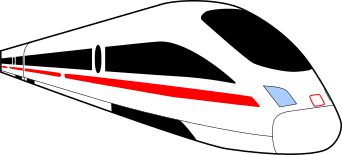
\includegraphics[scale=0.4]{img/analytic_geometry/train}} -- (2,-0.5) node[black, above, midway] {$\vec{v}$} node[sloped, pos=1, anchor=west] {direction};
\draw [decorate, decoration={brace, amplitude=5pt, mirror}, xshift=-2pt, yshift=-2pt] (0,0) -- (2,-0.5) node [midway, below, sloped, xshift=-2pt, yshift=-2pt] {magnitude};
\end{tikzpicture}

\end{center}
\end{frame}


% ---------------------------------------------------------------------slide----
\begin{frame}
\frametitle{Vector representation}
An oriented segment can be located in different places in a Cartesian space.  
However, regardless of where it is located, if the length and the direction of the segment does not change, the segment represents always the same vector. 

This allows to represent all vectors with the same origin, the origin of the Cartesian coordinate system.
Thus, a vector can be represented by the Cartesian \emph{coordinates} of its final end in any Euclidean space.

\begin{center}
\tikzsetnextfilename{analytic_geometry/vector_coordinates}
% Author: Alfredo Sánchez Alberca (asalber@ceu.es)
\begin{tikzpicture}[trim axis left, trim axis right]
  \begin{axis}[
    gen2dfun, 
    xmin=-4, xmax=4,
    ymin=-4, ymax=4,  
    xtick={3},
    xticklabels={$x_0$},
    ytick={2},
    yticklabels={$y_0$}, 
    clip=false,
    height=4cm,
    ]
    \coordinate (O) at (0,0);
    \coordinate (A) at (3,2);
    \draw[vector] (O) -- (A) node[midway, below, anchor=west] {$\mathbf{v}=(x_0,y_0)=\vec{AB}=\vec{CD}=\vec{EF}$} ;
    \draw[gray, dotted] (A) -- (A|-O);
    \draw[gray, dotted] (A) -- (A-|O);
    \draw[->] (2,2) -- (5,4) node[midway, above] {$\vec{AB}$};
    \draw[->] (-4,1) -- (-1,3) node[midway, above] {$\vec{CD}$};
    \draw[->] (-2,-3) -- (1,-1) node[midway, above] {$\vec{EF}$};
  \end{axis}
\end{tikzpicture}

\end{center}
\end{frame}


% ---------------------------------------------------------------------slide----
\begin{frame}
\frametitle{Vector from two points}
Given two points $P$ and $Q$ of a Cartesian space, the vector that starts at $P$ and ends at $Q$ has coordinates 
$\vec{PQ}=Q-P$.

\structure{\bfseries Example} Given the points $P=(1,1)$ and $Q=(3,4)$ in the real plane $\mathbb{R}^2$, the coordinates of the vector that start at $P$ and ends at $Q$ are
\[
\vec{PQ} = Q-P = (3,4)-(1,1) = (3-2,4-1) = (2,3).
\]
\begin{center}
\tikzsetnextfilename{analytic_geometry/vector_from_two_points}
% Author: Alfredo Sánchez Alberca (asalber@ceu.es)
\begin{tikzpicture}[trim axis left, trim axis right]
  \begin{axis}[
    2dfun, 
    xmin=-4, xmax=4,
    ymin=-4, ymax=4,  
    equal axis=true,
    height=4cm,
    ]
    \coordinate (0) at (0,0);
    \coordinate (P) at (2,1);
    \coordinate (Q) at (3,4);
    \draw[->, color1] (O) -- (A) node[midway, below, anchor=west] {$\vec{PQ}=(1,3)$} ;
    \draw[gray, dotted] (P) -- (P|-O);
    \draw[gray, dotted] (P) -- (P-|O);
    \draw[gray, dotted] (Q) -- (Q|-O);
    \draw[gray, dotted] (Q) -- (Q-|O);
  \end{axis}
\end{tikzpicture}

\end{center}
\end{frame}


% ---------------------------------------------------------------------slide----
\begin{frame}
\frametitle{Module of a vector}
\begin{definition}[Module of a vector]
Given a vector $\mathbf{v}=(v_1,\cdots,v_n)$ in $\mathbb{R}^n$, the \emph{module} of $\mathbf{v}$ is
\[
|\mathbf{v}| = \sqrt{v_1^2+ \cdots + v_n^2}.
\]
\end{definition}
The module of a vector coincides with the length of the segment that represents the vector.

\structure{\bfseries Examples}
Let $\mathbf{u}=(3,4)$ be a vector in $\mathbb{R}^2$, then its module is
\[
|\mathbf{u}| = \sqrt{3^2+4^2} = \sqrt{25} = 5
\]
Let $\mathbf{v}=(4,7,4)$ be a vector in $\mathbb{R}^3$, then its module is
\[
|\mathbf{v}| = \sqrt{4^2+7^2+4^2} = \sqrt{81} = 9
\]
\end{frame}


% ---------------------------------------------------------------------slide----
\begin{frame}
\frametitle{Unit vectors}
\begin{definition}[Unit vector]
A vector $\mathbf{v}$ in $\mathbb{R}^n$ is a \emph{unit vector} if its module is one, that is, $|\mathbf{v}|=1$.
\end{definition}

The unit vectors with the direction of the coordinate axes are of special importance and they form the \emph{standard basis}.

\begin{columns}
\begin{column}{.48\textwidth}
In $\mathbb{R}^2$ the standard basis is formed by two vectors
\[
\mathbf{i}=(1,0)\mbox{ and }\mathbf{j}=(0,1)
\]
\begin{center}
\tikzsetnextfilename{analytic_geometry/standard_basis_plane}
% Author: Alfredo Sánchez Alberca (asalber@ceu.es)
\begin{tikzpicture}[trim axis left, trim axis right]
  \begin{axis}[
    2dfun, 
    xmin=-0.2, xmax=2,
    ymin=-0.20, ymax=2, 
    axis equal=true,
    clip=false,
    height=3cm,
    ]
    \draw[vector] (0,0) -- (1,0) node[midway, above] {$\mathbf{i}$};
    \draw[vector] (0,0) -- (0,1) node[midway, right] {$\mathbf{j}$};
  \end{axis}
\end{tikzpicture}

\end{center}
\end{column}
\begin{column}{.48\textwidth}
In $\mathbb{R}^3$ the standard basis is formed by three vectors
\[
\mathbf{i}=(1,0,0)\mbox{, }\mathbf{j}=(0,1,0) \mbox{ and } \mathbf{k}=(0,0,1)
\]
\begin{center}
\tikzsetnextfilename{analytic_geometry/standard_basis_space}
% Author: Alfredo Sánchez Alberca (asalber@ceu.es)
\begin{tikzpicture}
  \begin{axis}[
  3dfun,
  xmin=-0.2, xmax=2,
  ymin=-0.2, ymax=2,
  zmin=-0.2, zmax=2,
  axis x line=middle,
  axis y line=middle,
  axis z line=middle,
  %axis equal=true,
  every axis x label/.style={at={(ticklabel cs:1)}, anchor=center,},
  every axis y label/.style={at={(ticklabel cs:1)}, anchor=center,},
  every axis z label/.style={at={(ticklabel cs:1)}, anchor=center,},
  clip=false,
  height=4cm,
  ]
  %\addplot3+[domain=0:pi, samples y=0] ({cos(deg(x))}, {sin(deg(x))}, {x});
  \coordinate (P) at (0,1,0);
  \draw [vector] (0,0,0) -- (1,0,0) node[anchor=west] {$\textbf{i}$};
  \draw [vector] (0,0,0) -- (0,1,0) node[anchor=west] {$\textbf{j}$};
  \draw [vector] (0,0,0) -- (0,0,1) node[anchor=west] {$\textbf{k}$};
  \end{axis}
\end{tikzpicture}

\end{center}
\end{column}
\end{columns}
\end{frame}


% ---------------------------------------------------------------------slide----
\begin{frame}
\frametitle{Sum of two vectors}
\begin{definition}[Sum of two vectors]
Given two vectors $\mathbf{u}=(u_1,\cdots,u_n)$ y $\mathbf{v}=(v_1,\cdots,v_n)$ de $\mathbb{R}^n$, the \emph{sum} of $\mathbf{u}$ and $\mathbf{v}$ is
\[
\mathbf{u}+\mathbf{v} = (u_1+v_1,\ldots, u_n+v_n).
\]
\end{definition}

\structure{\bfseries Example}
Let $\mathbf{u}=(3,1)$ and $\mathbf{v}=(2,3)$ two vectors in $\mathbb{R}^2$, then the sum of them is 
\[
\mathbf{u}+\mathbf{v} = (3+2,1+3) = (5,4).
\]

\begin{center}
\tikzsetnextfilename{analytic_geometry/sum_vectors}
% Author: Alfredo Sánchez Alberca (asalber@ceu.es)
\begin{tikzpicture}[trim axis left, trim axis right]
  \begin{axis}[
    gen2dfun, 
    xmin=0, xmax=4.5,
    ymin=0, ymax=4,
    xtick={1,3,4},
    xticklabels={$v_1$,$u_1$,$u_1+v_1$},
    ytick={1,2,3},
    yticklabels={$u_2$,$v_2$,$u_2+v_2$}, 
    %axis equal=true,
    clip=false,
    height=3cm,
    ]
    \coordinate (O) at (0,0);
    \coordinate (A) at (3,1);
    \coordinate (B) at (1,2);
    \coordinate (C) at ($(A)+(B)$);
    \draw[vector] (O) -- (A) node[midway, below] {$\mathbf{u}$} ;
    \draw[vector] (O) -- (B) node[midway, above] {$\mathbf{v}$} ;
    \draw[vector, color2] (O) -- (C) node[midway, above, sloped] {$\mathbf{u}+\mathbf{v}$} ;
    \draw[gray, dotted] (A) -- (A|-O);
    \draw[gray, dotted] (A) -- (A-|O);
    \draw[gray, dotted] (B) -- (B|-O);
    \draw[gray, dotted] (B) -- (B-|O);
    \draw[gray, dotted] (C) -- (C|-O);
    \draw[gray, dotted] (C) -- (C-|O);
    \draw[gray, dashed] (A) -- (C);
    \draw[gray, dashed] (B) -- (C);
  \end{axis}
\end{tikzpicture}

\end{center}
\end{frame}


%---------------------------------------------------------------------slide----
\begin{frame}
\frametitle{Product of a vector by a scalar}
\begin{definition}[Product of a vector by a scalar]
Given a vector $\mathbf{v}=(v_1,\cdots,v_n)$ in $\mathbb{R}^n$, and a scalar $a\in \mathbb{R}$, the \emph{product} of $\mathbf{v}$ by $a$ is 
\[
a\mathbf{v} = (av_1,\ldots, av_n).
\]
\end{definition}
\structure{\bfseries Example}
Let $\mathbf{v}=(2,1)$ a vector in $\mathbb{R}^2$ and $a=2$ a scalar, then the product of $a$ by $\mathbf{v}$ is
\[
a\mathbf{v} = 2(2,1) = (4,2).
\]

\begin{center}
\tikzsetnextfilename{analytic_geometry/product_vector_by_scalar}
% Author: Alfredo Sánchez Alberca (asalber@ceu.es)
\begin{tikzpicture}[trim axis left, trim axis right]
  \begin{axis}[
    gen2dfun, 
    xmin=0, xmax=4.5,
    ymin=0, ymax=3,
    xtick={2,4},
    xticklabels={$v_1$,$av_1$},
    ytick={1,2},
    yticklabels={$v_2$,$av_2$}, 
    axis equal=true,
    clip=false,
    height=3cm,
    ]
    \coordinate (O) at (0,0);
    \coordinate (A) at (2,1);
    \coordinate (C) at ($2*(A)$);
    \draw[vector, color2] (O) -- (C) node[midway, above, pos=0.6] {$a\mathbf{v}$} ;
    \draw[vector] (O) -- (A) node[midway, above] {$\mathbf{v}$} ;
    \draw[gray, dotted] (A) -- (A|-O);
    \draw[gray, dotted] (A) -- (A-|O);
    \draw[gray, dotted] (C) -- (C|-O);
    \draw[gray, dotted] (C) -- (C-|O);
  \end{axis}
\end{tikzpicture}

\end{center}
\end{frame}


%---------------------------------------------------------------------slide----
\begin{frame}
\frametitle{Expressing a vector as a linear combination of the standard basis}
The sum of vectors and the product of vector by a scalar allow us to express any vector as a linear combination of the standard basis. 

In $\mathbb{R}^3$, for instance, a vector with coordinates $\mathbf{v}=(v_1,v_2,v_3)$ can be expressed as the linear combination
\[
\mathbf{v}=(v_1,v_2,v_3) = v_1\mathbf{i}+v_2\mathbf{j}+v_3\mathbf{k}.
\]

\begin{center}
\tikzsetnextfilename{analytic_geometry/linear_combination_standard_basis}
% Author: Alfredo Sánchez Alberca (asalber@ceu.es)
\begin{tikzpicture}
  \begin{axis}[view={120}{20},
  gen3dfun,
  xmin=-0.2, xmax=2.2,
  ymin=-0.2, ymax=2,
  zmin=-0.2, zmax=3.2,
  axis x line=middle,
  axis y line=middle,
  axis z line=middle,
  axis equal=true,
  every axis x label/.style={at={(xticklabel* cs:1.1)}},
  every axis y label/.style={at={(yticklabel* cs:1.1)}},
  every axis z label/.style={at={(zticklabel* cs:1.1)}},
  x tick label style={anchor=east, inner sep=2pt}, 
  y tick label style={anchor=north, inner sep=5pt},
  z tick label style={anchor=east, inner sep=2pt},  
  xtick={1},
  xticklabels={$v_1$},
  ytick={2},
  yticklabels={$v_2$}, 
  ztick={3},
  zticklabels={$v_3$},
  clip=false,
  height=5cm,
  ]
  \coordinate (O) at (0,0,0);
  \coordinate (I) at (1,0,0);
  \coordinate (J) at (0,1,0);
  \coordinate (K) at (0,0,1);
  \coordinate (A) at (1,2,3);
  \draw [vector] (O) -- (I) node[anchor=west] {$\textbf{i}$};
  \draw [vector] (O) -- (J) node[anchor=west] {$\textbf{j}$};
  \draw [vector] (O) -- (K) node[anchor=west] {$\textbf{k}$};
  \draw [vector, color2] (O) -- (A) node[anchor=west] {$\textbf{v}$};
  \draw[gray, dotted] (I) -- (1,2,0);
  \draw[gray, dotted] (0,2,0) -- (1,2,0);
  \draw[gray, dotted] (0,2,0) -- (0,2,3);
  \draw[gray, dotted] (0,0,3) -- (0,2,3);
  \draw[gray, dotted] (I) -- (1,0,3);
  \draw[gray, dotted] (0,0,3) -- (1,0,3);
  \draw[gray, dotted] (1,2,0) -- (A);
  \draw[gray, dotted] (1,0,3) -- (A);
  \draw[gray, dotted] (0,2,3) -- (A);
  \end{axis}
\end{tikzpicture}

\end{center}
\end{frame}


%---------------------------------------------------------------------slide----
\begin{frame}
\frametitle{Dot product of two vectors}
\begin{definition}[Dot product of two vectors]
Given the vectors $\mathbf{u}=(u_1,\cdots,u_n)$ and $\mathbf{v}=(v_1,\cdots,v_n)$ in $\mathbb{R}^n$, the 
\emph{dot product} of $\mathbf{u}$ and $\mathbf{v}$ is
\[
\mathbf{u}\cdot \mathbf{v} = u_1v_1 + \cdots + u_nv_n.
\]
\end{definition}

\structure{\bfseries Example}
Let $\mathbf{u}=(3,1)$ and $\mathbf{v}=(2,3)$ two vectors in $\mathbb{R}^2$, then the dot product of them is
\[
\mathbf{u}\cdot\mathbf{v} = 3\cdot 2 +1\cdot 3 = 9.
\]

It holds that 
\[
\mathbf{u}\cdot\mathbf{v} =  |\mathbf{u}||\mathbf{v}|\cos\alpha
\]
where $\alpha$ is the angle between the vectors.
\end{frame}


%---------------------------------------------------------------------slide----
\begin{frame}
\frametitle{Parallel vectors}
\begin{definition}[Parallel vectors]
Two vectors $\mathbf{u}$ and $\mathbf{v}$ are \emph{parallel} if there is a scalar $a\in\mathbb{R}$ such that 
\[
\mathbf{u} = a\mathbf{v}.
\]
\end{definition}

\structure{\bfseries Example}
The vectors $\mathbf{u}=(-4,2)$ and $\mathbf{v}=(2,-1)$ in $\mathbb{R}^2$ are parallel, as there is a scalar $-2$ such that
\[
\mathbf{u}= (-4,2) = -2(2,-1) = -2\mathbf{v}.
\]
\end{frame}


%---------------------------------------------------------------------slide----
\begin{frame}
\frametitle{Orthogonal and orthonormal vectors}
\begin{definition}[Orthogonal and orthonormal vectors]
Two vectors $\mathbf{u}$ and $\mathbf{v}$ are \emph{orthogonal} if their dot product is zero,
\[
\mathbf{u}\cdot \mathbf{v} = 0.
\]
If in addition both vectors are unit vectors, $|\mathbf{u}|=|\mathbf{v}|=1$, then the vectors are \emph{orthonormal}.
\end{definition}

Orthogonal vectors are perpendicular, that is the angle between them is right.

\structure{\bfseries Example}
The vectors $\mathbf{u}=(2,1)$ and $\mathbf{v}=(-2,4)$ in $\mathbb{R}^2$ are orthogonal, as
\[
\mathbf{u}\mathbf{v} = 2\cdot -2 +1\cdot 4 = 0,
\]
but they are not orthonormal since $|\mathbf{u}| = \sqrt{2^2+1^2} \neq 1$ and $|\mathbf{v}| = \sqrt{-2^2+4^2} \neq 1$.

The vectors $\mathbf{i}=(1,0)$ and $\mathbf{j}=(0,1)$ in $\mathbb{R}^2$ are orthonormal, as
\[
\mathbf{i}\mathbf{j} = 1\cdot 0 +0\cdot 1 = 0, \quad |\mathbf{i}| = \sqrt{1^2+0^2} = 1,  \quad |\mathbf j| = \sqrt{0^2+1^2} = 1.
\]
\end{frame}



\subsection{Lines}
%---------------------------------------------------------------------slide----
\begin{frame}
\frametitle{Vectorial equation of a straight line}
\begin{definition}[Vectorial equation of a straight line]
Given a point $P=(p_1,\ldots,p_n)$ and a vector $\mathbf{v}=(v_1,\ldots,v_n)$ of $\mathbb{R}^n$, the \emph{vectorial equation of the line} $l$ that passes through the point $P$ with the direction of $\mathbf{v}$ is
\[
l: X= P + t\mathbf{v} = (p_1,\ldots,p_n)+t(v_1,\ldots,v_n) = (p_1+tv_1,\ldots,p_n+tv_n),\quad t\in\mathbb{R}.
\]
\end{definition}
%This equation is a parameterises $l$ as a function of the parameter $t\in \mathbb{R}$.

\begin{columns}
\begin{column}{.48\textwidth}
\structure{\bfseries Example}
Let $l$ the line of $\mathbb{R}^3$ that goes through $P=(1,1,2)$ with the direction of $\mathbf{v}=(3,1,2)$, then the vectorial equation of $l$ is
\begin{align*}
l &: X= P + t\mathbf{v} = (1,1,2)+t(3,1,2) =\\
&= (1+3t,1+t,2+2t)\quad t\in\mathbb{R}.
\end{align*}
\end{column}
\begin{column}{.48\textwidth}
\begin{center}
\tikzsetnextfilename{analytic_geometry/vectorial_equation_line}
% Author: Alfredo Sánchez Alberca (asalber@ceu.es)
\begin{tikzpicture}
  \begin{axis}[%view={120}{20},
  3dfun,
  xmin=-0.2, xmax=5,
  ymin=-0.2, ymax=5,
  zmin=-0.2, zmax=5,
  %axis x line=middle,
  %axis y line=middle,
  %axis z line=middle,
  % axis equal=true,
  %every axis x label/.style={at={(ticklabel cs:1.08,-12pt)}, anchor=center},
  %every axis y label/.style={at={(ticklabel cs:1.03,-15pt)}, anchor=center},
  %every axis z label/.style={at={(ticklabel cs:1.03,-15pt)}, anchor=south},
  %x tick label style={anchor=east, inner sep=2pt}, 
  %y tick label style={anchor=north, inner sep=5pt},
  %z tick label style={anchor=east, inner sep=2pt},  
  clip=false,
  height=3cm,
  ]
  \coordinate (O) at (0,0,0);
  \coordinate (P) at (1,1,2);
  \fill (P) circle (1.2pt) node[anchor=south] {$P$};
  \addplot3+[domain=-0.4:1.4] ({1+3*x}, {1+x)}, {2+2*x}) node[anchor=south west] {$l$};
  \draw [vector, color2] (P) -- (4,2,4) node[midway, above] {$\textbf{v}$};
  \end{axis}
\end{tikzpicture}

\end{center}
\end{column}
\end{columns}
\end{frame}


%---------------------------------------------------------------------slide----
\begin{frame}
\frametitle{Parametric and Cartesian equations of a line}
From the vectorial equation of a line $l: X=P + t\mathbf{v}=(p_1+tv_1,\ldots,p_n+tv_n)$ is easy to obtain the coordinates of the the points of the line with $n$ \emph{parametric equations}
\[
x_1(t)=p_1+tv_1, \ldots, x_n(t)=p_n+tv_n
\]
from where, if $\mathbf{v}$ is a vector with non-null coordinates ($v_i\neq 0$ $\forall i$), we can solve for $t$ and equal the equations getting the \emph{Cartesian equations}  
\[
\frac{x_1-p_1}{v_1}=\cdots = \frac{x_n-p_n}{v_n}
\]

\structure{\bfseries Example}
Given a line with vectorial equation $l: X=(1,1,2)+t(3,1,2) =(1+3t,1+t,2+2t)$ in $\mathbb{R^3}$, its parametric equations are 
\[
x(t) = 1+3t, \quad y(t)=1+t, \quad z(t)=2+2t,
\]
and the Cartesian equations are
\[
\frac{x-1}{3}=\frac{y-1}{1}=\frac{z-2}{2}
\]
\end{frame}


%---------------------------------------------------------------------slide----
\begin{frame}
\frametitle{Point-slope equation of a line in the plane}
In the particular case of the real plane $\mathbb{R}^2$, if we have a line with vectorial equation $l: X=P+t\mathbf{v}=(x_0,y_0)+t(a,b)
= (x_0+ta,y_0+tb)$, its parametric equations are
\[
x(t)=x_0+ta,\quad y(t)=y_0+tb
\]
and its Cartesian equation is
\[
\frac{x-x_0}{a} = \frac{y-y_0}{b}.
\]
From this, moving $b$ to the other side of the equation, we get 
\[
y-y_0 = \frac{b}{a}(x-x_0),
\]
or renaming $m=b/a$,
\[
y-y_0=m(x-x_0).
\]
This equation is known as the \emph{point-slope equation} of the line.
\end{frame}


%---------------------------------------------------------------------slide----
\begin{frame}
\frametitle{Slope of a line in the plane}
\begin{definition}[Slope of a line in the plane]
Given a line $l: X=P+t\mathbf{v}$ in the real plane $\mathbb{R}^2$, with direction vector $\mathbf{v}=(a,b)$, the \emph{slope} of $l$ is $b/a$.
\end{definition}

Recall that given two points $P=(x_1,y_1)$ and $Q=(x_2,y_2)$ on the line $l$, we can take as a direction vector the vector from $P$ to $Q$, with coordinates $\vec{PQ}=Q-P=(x_2-x_1,y_2-y_1)$. 
Thus, the slope of $l$ is $\dfrac{y_2-y_1}{x_2-x_1}$, that is, the ratio between the changes in the vertical and horizontal axes.
\begin{center}
\tikzsetnextfilename{analytic_geometry/line_slope}
% Author: Alfredo Sánchez Alberca (asalber@ceu.es)
\begin{tikzpicture}
  \begin{axis}[
  gen2dfun,
  xmin=0, xmax=5,
  ymin=0, ymax=4,
  axis equal=true,
  xtick={1,4},
  xticklabels={$x_1$, $x_2$},
  ytick={1,3},
  yticklabels={$y_1$, $y_2$}, 
  clip=false,
  height=3cm,
  ]
  \coordinate (O) at (0,0);
  \coordinate (P) at (1,1);
  \coordinate (Q) at (4,3);
  \fill (P) circle (1.2pt) node[anchor=south] {$P$};
  \fill (Q) circle (1.2pt) node[anchor=south] {$Q$};
  \addplot+[domain=-0.3:1.3] ({1+3*x},{1+2*x}) node[anchor=south west] {$l$};
  \draw [vector, color2] (P) -- (Q) node[midway, above] {$\vec{PQ}$};
  \draw[gray, dotted] (P) -- (P-|O);
  \draw[gray, dotted] (P) -- (P|-O);
  \draw[gray, dotted] (Q) -- (Q-|O);
  \draw[gray, dotted] (Q) -- (Q|-O);
  \draw[gray, dashed] (Q) -- (Q|-P);
  \draw[gray, dashed] (P) -- (P-|Q);
  \draw[decorate, decoration={brace, amplitude=5pt}] (Q) -- (Q|-P) node [midway, right, xshift=4pt] {$y_2-y_1$};
  \draw[decorate, decoration={brace, amplitude=5pt, mirror}] (P) -- (P-|Q) node [midway, below, yshift=-4pt] {$x_2-x_1$};
  \end{axis}
\end{tikzpicture}

\end{center}
\end{frame}



\subsection{Planes}
%---------------------------------------------------------------------slide----
\begin{frame}
\frametitle{Vector equation of a plane in space}
To get the equation of a plane in the real space $\mathbb{R}^3$ we can take a point of the plane $P=(x_0,y_0,z_0)$ and an orthogonal vector to the plane $\mathbf{v}=(a,b,c)$.
Then, any point $Q=(x,y,z)$ of the plane satisfies that the vector $\vec{PQ} = (x-x_0,y-y_0,z-z_0)$ is orthogonal to $\mathbf{v}$, and therefore their dot product is zero. 
\[
\vec{PQ}\cdot\mathbf{v} = (x-x_0,y-y_0,z-z_0)(a,b,c) = a(x-x_0)+b(y-y_0)+c(z-z_0) = 0.
\]
This equation is known as the \emph{vector equation of the plane}.

\begin{center}
\tikzsetnextfilename{analytic_geometry/plane_equation}
% Author: Alfredo Sánchez Alberca (asalber@ceu.es)
\begin{tikzpicture}
  \begin{axis}[%view={120}{20},
  gen3dfun,
  xmin=0, xmax=5,
  ymin=0, ymax=4,
  zmin=0, zmax=4,
  %enlargelimits=false,
  %axis x line=middle,
  %axis y line=middle,
  %axis z line=middle,
  %axis equal=true,
  every axis x label/.style={at={(ticklabel cs:0.5,12pt)}, anchor=center},
  every axis y label/.style={at={(ticklabel cs:0.5,12pt)}, anchor=center},
  every axis z label/.style={at={(ticklabel cs:0.5,12pt)}, anchor=center},
  %x tick label style={anchor=east, inner sep=2pt}, 
  %y tick label style={anchor=north, inner sep=5pt},
  %z tick label style={anchor=east, inner sep=2pt},
  ticks=none,  
  clip=false,
  height=4cm,
  ]
  \coordinate (O) at (0,0,0);
  \coordinate (P) at (2,2,0.5);
  \coordinate (Q) at (3,2,-0.5);
  \fill (P) circle (1.2pt) node[anchor=south] {$P$};
  \fill (Q) circle (1.2pt) node[anchor=south] {$Q$};
  \addplot3[surf, domain=0:4, y domain=-1:5, samples=2, opacity=0.5, fill=color1, faceted color=color1] {(-2*x-y+7)/2};
  \draw [vector, color2] (P) -- (4,2,3) node[midway, above] {$\textbf{v}$};
  \draw [vector] (P) -- (Q) node[midway, below, anchor=east] {$\vec{PQ}$};
  \end{axis}
\end{tikzpicture}

\end{center}
\end{frame}


%---------------------------------------------------------------------slide----
\begin{frame}
\frametitle{Scalar equation of a plane in space}
From the vector equation of the plane we can get
\[
a(x-x_0)+b(y-y_0)+c(z-z_0) = 0 \Leftrightarrow ax+by+cz=ax_0+by_0+cz_0,
\]
that, renaming $d=ax_0+by_0+cz_0$, can be written as
\[
ax+by+cz=d,
\]
and is known as the \emph{scalar equation of the plane}.

\structure{\bfseries Example} Given the point $P=(2,1,1)$ and the vector $\mathbf{v}=(2,1,2)$, the vector equation of the plane that passes through $P$ and is orthogonal to $\mathbf{v}$ is
\[
(x-2,y-1,z-1)(2,1,2)=2(x-2)+(y-1)+2(z-1)=0,
\]
and its scalar equation is 
\[
2x+y+2z=7.
\] 
\end{frame}




% Author: Alfredo Sánchez Alberca (asalber@ceu.es)
% !TEX root = ../calculus_manual.tex
\section{Differential calculus with one real variable}

\mode<presentation>{
	%---------------------------------------------------------------------slide----
	\begin{frame}
		\frametitle{Differential calculus with one variable}
		\tableofcontents[sectionstyle=show/hide,hideothersubsections]
	\end{frame}
}


\subsection{Concept of derivative}
%---------------------------------------------------------------------slide----
\begin{frame}
	\frametitle{Increment}
	\begin{definition}[Increment of a variable]
		An \emph{increment} of a variable $x$ is a change in the value of the variable; is it is denoted $\Delta x$.
		The increment of a variable $x$ along an interval $[a,b]$ is given by
		\[
			\Delta x = b-a.
		\]
	\end{definition}
	
	\begin{definition}[Increment of a function]
		The \emph{increment} of a function $y=f(x)$ along an interval $[a,b]\subseteq Dom(f)$ is given by
		\[
			\Delta y = f(b)-f(a).
		\]
	\end{definition}
	
	\textbf{Example} The increment of $x$ along the interval $[2,5]$ is $\Delta x=5-2=3$ and the increment of the function $y=x^2$ along the same interval is $\Delta y=5^2-2^2=21$.
\end{frame}

\begin{frame}
	\frametitle{Average rate of change}
	The study of a function $y=f(x)$ requires to understand how the function changes, that is, how the dependent variable $y$ changes when we change the independent variable $x$.
	
	\begin{definition}[Average rate of change]
		The  \emph{average rate of change} of a function $y=f(x)$ in an interval $[a,a+\Delta x]\subseteq Dom(f)$, is the quotient between the increment of $y$ and the increment of $x$ in that interval, and is denoted by
		\[
			\mbox{ARC}\;f[a,a+\Delta x]=\frac{\Delta y}{\Delta x}=\frac{f(a+\Delta x)-f(a)}{\Delta x}.
		\]
	\end{definition}
\end{frame}

%---------------------------------------------------------------------slide----
\begin{frame}
	\frametitle{Average rate of change}
	\framesubtitle{Example of the area of a square}
	Let $y=x^2$ be the function that measures the area of a metallic square of side length $x$.
	
	If at any given time the side of the square is $a$, and we heat the square uniformly increasing the side by dilatation a quantity $\Delta x$, how much will the area of the square increase?
	\begin{columns}
		\begin{column}{0.3\textwidth}
			\begin{align*}
				\Delta y & = f(a+\Delta x)-f(a)=(a+\Delta x)^2-a^2=\\
				         & = a^2+2a\Delta x+\Delta x^2-a^2=2a\Delta x+\Delta x^2. 
			\end{align*}
		\end{column}
		\begin{column}{0.3\textwidth}
			\begin{center}
				\tikzsetnextfilename{derivatives_1_variable/square_area_variation}
				\mode<article>{\resizebox{0.3\textwidth}{!}{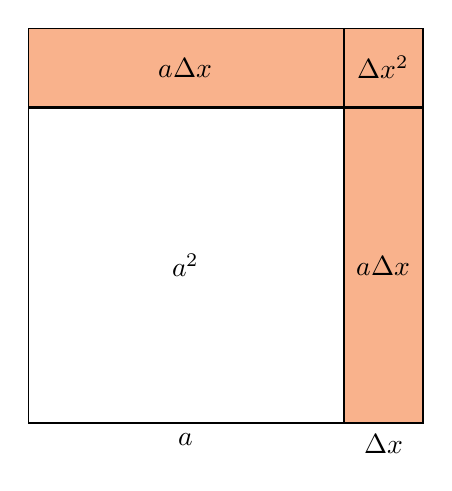
\begin{tikzpicture}
% \draw (0,0) node[below] {$a$} rectangle (4,4) node[midway] {$a^2$};
% \draw [fill=orange] (0,4) rectangle (4,5) node[midway] {$a\Delta x$};
% \draw [fill=orange] (4,0) rectangle (5,4) node[midway] {$a\Delta x$};
% \draw [fill=orange] (4,4) rectangle (5,5) node[midway] {$\Delta x^2$};
\node (A) [rectangle, draw, minimum width=4cm, minimum height=4cm, label={[anchor=north]south:$a$}] at (0,0) {$a^2$};
\node (B) [anchor=south, rectangle, draw, fill=color4!50, minimum width=4cm, minimum height=1cm] at (A.north) {$a\Delta x$};
\node (C) [anchor=west, rectangle, draw, fill=color4!50, minimum width=1cm, minimum height=4cm, label={[anchor=north]south:$\Delta x$}] at (A.east) {$a\Delta x$};
\node (D) [anchor=south, rectangle, draw, fill=color4!50, minimum width=1cm, minimum height=1cm] at (C.north) {$\Delta x^2$};
\end{tikzpicture}
}}
				\mode<presentation>{\resizebox{0.9\textwidth}{!}{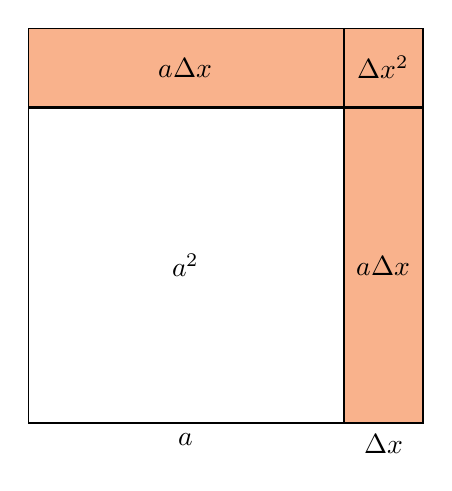
\begin{tikzpicture}
% \draw (0,0) node[below] {$a$} rectangle (4,4) node[midway] {$a^2$};
% \draw [fill=orange] (0,4) rectangle (4,5) node[midway] {$a\Delta x$};
% \draw [fill=orange] (4,0) rectangle (5,4) node[midway] {$a\Delta x$};
% \draw [fill=orange] (4,4) rectangle (5,5) node[midway] {$\Delta x^2$};
\node (A) [rectangle, draw, minimum width=4cm, minimum height=4cm, label={[anchor=north]south:$a$}] at (0,0) {$a^2$};
\node (B) [anchor=south, rectangle, draw, fill=color4!50, minimum width=4cm, minimum height=1cm] at (A.north) {$a\Delta x$};
\node (C) [anchor=west, rectangle, draw, fill=color4!50, minimum width=1cm, minimum height=4cm, label={[anchor=north]south:$\Delta x$}] at (A.east) {$a\Delta x$};
\node (D) [anchor=south, rectangle, draw, fill=color4!50, minimum width=1cm, minimum height=1cm] at (C.north) {$\Delta x^2$};
\end{tikzpicture}
}}
			\end{center}
		\end{column}
	\end{columns}
	What is the average rate of change in the interval $[a,a+\Delta x]$?
	\[
		\mbox{ARC}\;f[a,a+\Delta x]=\frac{\Delta y}{\Delta x}=\frac{2a\Delta x+\Delta x^2}{\Delta x}=2a+\Delta x.
	\]
\end{frame}


%---------------------------------------------------------------------slide----
\begin{frame}
	\frametitle{Geometric interpretation of the average rate of change}
	The average rate of change of a function $y=f(x)$ in an interval $[a,a+\Delta x]$ is the slope of the \emph{secant} line to the graph of $f$ through the points $(a,f(a))$ and $(a+\Delta x,f(a+\Delta x))$.
	\begin{center}
		\tikzsetnextfilename{derivatives_1_variable/secant_line}
		% Author: Alfredo Sánchez Alberca (asalber@ceu.es)
\begin{tikzpicture}
  \begin{axis}[
    gen2dfun, 
    xmin=0, xmax=4.5,
    ymin=0, ymax=4,
    axis equal=true,  
    xtick={1,3},
    xticklabels={$a$,$a+\Delta x$},
    ytick={1,2.5},
    yticklabels={$f(a)$,$f(a+\Delta x)$}, 
%   ticks=none,
% 	extra y ticks={0.5,0.3},
% 	extra y tick labels={$f(a)$, $f(a+\Delta x)$},
% 	extra x ticks={0.5, 3},
% 	extra x tick labels={$a$,$a+\Delta x$},
    height=5cm,
    ]
    \addplot+[domain=0.2:3.5, smooth, name path=F] {2^(x-2)+0.5} node[anchor=south] {$f(x)$};
    \addplot+[domain=0.2:3.5, smooth, name path=S] {1+1.5/2*(x-1)} node[anchor=west] {Secant};
    \fill [name intersections={of=F and S, by={A,B}}]
      (A) circle (1.2pt)
      (B) circle (1.2pt);
    \coordinate (O);
    \draw[gray, dotted] (A) -- (A|-O);
    \draw[gray, dotted] (A) -- (A-|O);
    \draw[gray, dotted] (B) -- (B|-O);
    \draw[gray, dotted] (B) -- (B-|O);
    \draw (A) -- (A-|B) node [midway, below] {$\Delta x$};
    \draw (B) -- (B|-A) node [midway, right] {$\Delta y$};
  \end{axis}
\end{tikzpicture}

	\end{center}
\end{frame} 


%---------------------------------------------------------------------slide----
\begin{frame}
	\frametitle{Equation of the secant line}
  Since the average rate of change is the slope of the secant line, we can use it to define the equation of the secant line in the point-slope form.
  	  
	\begin{definition}[Equation of the secant line of a function]
    The equation of the \emph{secant line} of a function $f(x)$ at points $x=a$ and $x=a+\Delta x$, is 
    \[
			y=f(a)+\mbox{ARC}\;f[a,a+\Delta x](x-a) 
		\]
	\end{definition}
\end{frame}
  

%---------------------------------------------------------------------slide----
\begin{frame}
	\frametitle{Instantaneous rate of change}
	Often it is interesting to study the rate of change of a function, not in an interval, but in a point.
	
	Knowing the tendency of change of a function in an instant can be used to predict the value of the function in nearby instants.
	
	\begin{definition}[Instantaneous rate of change and derivative]
		The \emph{instantaneous rate of change} of a function $f(x)$ at a point $x=a$, is the limit of the average rate of change of $f$ in the interval $[a,a+\Delta x]$, when $\Delta x$ tends to 0, and is denoted by
		\[
			\mbox{IRC}\;f (a)=\lim_{\Delta x\rightarrow 0} \mbox{ARC}\; f[a,a+\Delta x]=\lim_{\Delta x\rightarrow 0}\frac{\Delta y}{\Delta x}=\lim_{\Delta x\rightarrow 0}\frac{f(a+\Delta x)-f(a)}{\Delta x}
		\]
		When this limit exists, the function $f$ is said to be \emph{differentiable} at the point $a$, and its value is called the \emph{derivative} of $f$ at $a$, and it is denoted $f'(a)$ (Lagrange's notation) or $\frac{df}{dx}(a)$ (Leibniz's notation).
	\end{definition}
\end{frame}


%---------------------------------------------------------------------slide----
\begin{frame}
	\frametitle{Instantaneous rate of change}
	\framesubtitle{Example of the area of a square}
	Let's take again the function $y=x^2$ that measures the area of a metallic square of side length $x$.
	
	If at any given time the side of the square is $a$, and we heat the square uniformly increasing the side, what is the tendency of change of the area in that moment?
	\begin{align*}
		\mbox{IRC}\;f(a) & =\lim_{\Delta x\rightarrow 0}\frac{\Delta y}{\Delta x}=\lim_{\Delta x\rightarrow 0}\frac{f(a+\Delta x)-f(a)}{\Delta x} = \\
		                 & =\lim_{\Delta x\rightarrow 0}\frac{2a\Delta x+\Delta x^2}{\Delta x}=\lim_{\Delta x\rightarrow 0} 2a+\Delta x= 2a.        
	\end{align*}
	Thus,
	\[
		f'(a)=\frac{df}{dx}(a)=2a,
	\]
	indicating that the area of the square tends to increase the double of the side.
\end{frame}


%---------------------------------------------------------------------slide----
\begin{frame}
	\frametitle{Interpretation of the derivative}
	The derivative of a function $f'(a)$ shows the growth rate of $f$ at point $a$:
	\begin{itemize}
		\item $f'(a)>0$ indicates an increasing tendency ($y$ increases as $x$ increases).
		\item $f'(a)<0$ indicates a decreasing tendency ($y$ decreases as $x$ increases).
	\end{itemize}
	
	\structure{\textbf{Example}} A derivative $f'(a)=3$ indicates that $y$ tends to increase triple of $x$ at point $a$. 
	A derivative $f'(a)=-0.5$ indicates that $y$ tends to decrease half of $x$ at point $a$. 
\end{frame}


%---------------------------------------------------------------------slide----
\begin{frame}
	\frametitle{Geometric interpretation of the derivative}
	\mode<article>{We have seen that the average rate of change of a function $y=f(x)$ in an interval $[a,a+\Delta x]$ is the slope of the \emph{secant} line, but when $\Delta x$ tends to $0$, the secant line becomes the tangent line.}
	
	The instantaneous rate of change or derivative of a function $y=f(x)$ at $x=a$ is the slope of the \emph{tangent line} to the graph of $f$ at point $(a,f(a))$. 
	Thus, the equation of the tangent line to the graph of $f$ at the point $(a,f(a))$ is
	
	\begin{center}
		\tikzsetnextfilename{derivatives_1_variable/tangent_line}
		% Author: Alfredo Sánchez Alberca (asalber@ceu.es)
\begin{tikzpicture}
  \begin{axis}[
    gen2dfun, 
    xmin=0, xmax=4.5,
    ymin=0, ymax=4,
    axis equal=true,  
    xtick={1},
    xticklabels={$a$},
    ytick={1},
    yticklabels={$f(a)$}, 
    height=5cm,
    ]
    \addplot+[domain=0.2:3.5, smooth, name path=F] {2^(x-2)+0.5} node[anchor=south] {$f(x)$};
    \addplot+[domain=0.2:3.5, smooth, name path=T] {1+ln(2)/2*(x-1)} node[anchor=north west, pos=0.8] {Tangent} node [anchor=north, pos=0.8] {$y=f(a)+f'(a)(x-a)$};
    \coordinate (O);
    \coordinate (A) at (1,1);
    \fill (A) circle (1.2pt);
    \draw[gray, dotted] (A) -- (A|-O);
    \draw[gray, dotted] (A) -- (A-|O);
  \end{axis}
\end{tikzpicture}

	\end{center}
\end{frame}


%---------------------------------------------------------------------slide----
\begin{frame}
	\frametitle{Equation of the tangent line}
  Since the derivative is the slope of the tangent line, we can use it to define the equation of the tangent line in the point-slope form.
  	  
	\begin{definition}[Equation of the tangent line of a function]
    The equation of the \emph{tangent line} of a function $f(x)$ at points $x=a$, is 
    \[
      y = f(a)+f'(a)(x-a)
    \]
	\end{definition}
\end{frame}


% ---------------------------------------------------------------------slide----
\begin{frame}
	\frametitle{Kinematic applications: Linear motion}
	Assume that the function $y=f(t)$ describes the position of an object moving in the real line at time $t$.
	Taking as reference the coordinates origin $O$ and the unitary vector $\mathbf{i}=(1)$, we can represent the position of the moving object $P$ at every moment $t$ with a vector $\vec{OP}=x\mathbf{i}$ where $x=f(t)$.
	\begin{center}
		\tikzsetnextfilename{derivatives_1_variable/linear_motion}
		% Author: Alfredo Sánchez Alberca (asalber@ceu.es)
\begin{tikzpicture}
\draw (0,0) -- (2,0) node[midway, above=0.5] {Time};
\draw (4,0) -- (8,0) node[midway, above=0.5] {Position} node[right] {$\mathbb{R}$};
\draw (1,0.1) -- (1,-0.1) node[anchor=north] (A) {$t$};
\draw (5,0.1) -- (5,-0.1) node[anchor=north] {$O$};
\draw (6,0.1) -- (6,-0.1) node[anchor=north] {$1$};
\draw [->, color1] (5,0) -- (7,0);
\draw [->, color2] (5,0) -- (6,0) node[midway, above] {\color{color2}$\mathbf{i}$};
\fill (7,0) circle (1.2pt) node[above] {$P$} node[anchor=north, xshift=2.5ex] (P) {$x=f(t)$};
\path [->, dashed] (A) edge[bend right] node[above] {$f$} (P);
\end{tikzpicture}

	\end{center}
	
	\structure{\textbf{Remark}} It also makes sense when $f$ measures other magnitudes as the temperature of a body, the concentration of a gas, or the quantity of substance in a chemical reaction at every moment $t$.
\end{frame}


% ---------------------------------------------------------------------slide----
\begin{frame}
	\frametitle{Kinematic interpretation of the average rate of change}
	In this context, if we take the instants $t=a$ and $t=a+\Delta t$, both in $\mbox{Dom}(f)$, the vector
	\[
		\mathbf{v}_m=\frac{f(a+\Delta t)-f(a)}{\Delta t}
	\]
	is known as the \emph{average velocity} of the trajectory $f$ in the interval $[a, a+\Delta t]$.
	
	\structure{\textbf{Example}}
	A vehicle makes a trip from Madrid to Barcelona.
	Let $f(t)$ be the function that determine the position of the vehicle at every moment $t$.
	If the vehicle departs from Madrid (km 0) at 8:00 and arrives at Barcelona (km 600) at 14:00, then the average velocity
	of the vehicle in the path is
	\[
		\mathbf{v}_m=\frac{f(14)-f(8)}{14-8}=\frac{600-0}{6} = 100 km/h.
	\]
\end{frame}


% ---------------------------------------------------------------------slide----
\begin{frame}
	\frametitle{Kinematic interpretation of the derivative}
	In the same context of the linear motion, the derivative of the function $f(t)$ at the moment $t_0$ is the vector
	\[
		\mathbf{v}=f'(a)=\lim_{\Delta t\rightarrow 0}\frac{f(a+\Delta t)-f(a)}{\Delta t},
	\]
	that is known, as long as the limit exists, as the \emph{instantaneous velocity} or simply \emph{velocity} of the trajectory $f$ at moment $a$.
	
	That is, the derivative of the object position with respect to time is a vector field that is called \emph{velocity along the trajectory $f$}.
	
	\structure{\textbf{Example}}
	Following with the previous example, what indicates the speedometer at any instant is the modulus of the instantaneous velocity vector at that moment.
\end{frame}


\subsection{Algebra of derivatives}
%---------------------------------------------------------------------slide----
\begin{frame}
	\frametitle{Properties of the derivative}
	If $y=c$, is a constant function, then $y'=0$ at any point.
	
	If $y=x$, is the identity function, then  $y'=1$ at any point.
	
	If $u=f(x)$ and $v=g(x)$ are two differentiable functions, then 
	\begin{itemize}
		\item $(u+v)'=u'+v'$
		\item $(u-v)'=u'-v'$
		\item $(u\cdot v)'=u'\cdot v+ u\cdot v'$
		\item $\left(\dfrac{u}{v}\right)'=\dfrac{u'\cdot v-u\cdot v'}{v^2}$
	\end{itemize}
\end{frame}


%---------------------------------------------------------------------slide----
\begin{frame}
	\frametitle{Derivative of a composite function}
	\framesubtitle{The chain rule}
	\begin{theorem}[Chain rule] If the function $y=f\circ g$ is the composition of two functions $y=f(z)$ and $z=g(x)$, then
		\[ 
			(f\circ g)'(x)=f'(g(x))g'(x).
		\]
	\end{theorem}
	
	It is easy to prove this fact using the Leibniz notation
	\[
		\frac{dy}{dx}=\frac{dy}{dz}\frac{dz}{dx}=f'(z)g'(x)=f'(g(x))g'(x).
	\]
	
	\structure{\textbf{Example}} If $f(z)=\sin z$ and $g(x)=x^2$, then $f\circ g(x)=\sin(x^2)$. Applying the chain rule the derivative of the composite function is
	\[
		(f\circ g)'(x)=f'(g(x))g'(x) = \cos(g(x)) 2x = \cos(x^2)2x.
	\]
	On the other hand, $g\circ f(z)= (\sin z)^2$, and applying the chain rule again, its derivative is
	\[
		(g\circ f)'(z)=g'(f(z))f'(z) = 2f(z)\cos z = 2\sin z\cos z.
	\]
\end{frame}


%---------------------------------------------------------------------slide----
\begin{frame}
	\frametitle{Derivative of the inverse of a function}
	\begin{theorem}[Derivative of the inverse function]
		Given a function $y=f(x)$ with inverse $x=f^{-1}(y)$, then 
		\[
			\left(f^{-1}\right)'(y)=\frac{1}{f'(x)}=\frac{1}{f'(f^{-1}(y))},
		\]
		provided that $f$ is differentiable at $f^{-1}(y)$ and $f'(f^{-1}(y))\neq 0$.
	\end{theorem}
	
	Again, it is easy to prove this equality using the Leibniz notation
	\[
		\frac{dx}{dy}=\frac{1}{dy/dx}=\frac{1}{f'(x)}=\frac{1}{f'(f^{-1}(y))}
	\]
\end{frame}


%---------------------------------------------------------------------slide----
\begin{frame}
	\frametitle{Derivative of the inverse of a function}
	\framesubtitle{Example}
	The inverse of the exponential function $y=f(x)=e^x$ is the natural logarithm $x=f^{-1}(y)=\ln y$, so we can compute the derivative of the natural logarithm using the previous theorem and we get
	\[
		\left(f^{-1}\right)'(y)=\frac{1}{f'(x)}=\frac{1}{e^x}=\frac{1}{e^{\ln y}}=\frac{1}{y}.
	\]
	
	\structure{\textbf{Example}} Sometimes it is easier to apply the chain rule to compute the derivative of the inverse of a function. 
	In this example, as $\ln x$ is the inverse of $e^x$, we know that $e^{\ln x}=x$, so differentiating both sides and applying the chain rule to the left side we get
	\[
		(e^{\ln x})'=x' \Leftrightarrow e^{\ln x}(\ln(x))' = 1 \Leftrightarrow (\ln(x))'=\frac{1}{e^{\ln x}}=\frac{1}{x}.
	\]
\end{frame}



\subsection{Analysis of functions}
%---------------------------------------------------------------------slide----
\begin{frame}
	\frametitle{Analysis of functions: increase and decrease}
	The main application of derivatives is to determine the variation (increase or decrease) of functions. 
	For that we use the sign of the first derivative.  
	\begin{theorem}
		Let $f(x)$ be a function with first derivative in an interval $I\subseteq \mathbb{R}$.
		\begin{itemize}
			\item If $\forall x\in I\ f'(x)> 0$ then $f$ is increasing on $I$.
			\item If $\forall x\in I\ f'(x)< 0$ then $f$ is decreasing on $I$.
		\end{itemize}
	\end{theorem}
	If $f'(a)=0$ then $a$ is known as a \emph{critical point} or \emph{stationary point}.
	At this point the function can be increasing, decreasing or neither increasing nor decreasing. 
	
	\structure{\textbf{Example}}
	The function $f(x)=x^2$ has derivative $f'(x)=2x$; it is decreasing on $\mathbb{R}^-$ as $f'(x)< 0$ $\forall x\in \mathbb{R}^-$  and increasing on $\mathbb{R}^+$ as $f'(x)> 0$ $\forall x\in \mathbb{R}^+$.
	
	It has a critical point at $x=0$, as $f'(0)=0$; at this point the function is neither increasing nor decreasing.
	
	\structure{\textbf{Remark}} {A function can be increasing or decreasing on an interval and not have first derivative.}
\end{frame}


%---------------------------------------------------------------------slide----
\begin{frame}
	\frametitle{Analysis of functions: increase and decrease}
	\framesubtitle{Example}
	Let us analyze the increase and decrease of the function $f(x)=x^4-2x^2+1$. 
	Its first derivative is $f'(x)=4x^3-4x$.
	\begin{center}
		\tikzsetnextfilename{derivatives_1_variable/increase_analysis}
		\scalebox{0.9}{% Author: Alfredo Sánchez Alberca (asalber@ceu.es)
\begin{tikzpicture}
  \begin{axis}[
    2dfun, 
    xmin=-2, xmax=2,
    ymin=-2, ymax=2,
    axis equal=true,
    clip=false, 
    width=5cm,
    ]
    \addplot+[domain=-1.5:1.5, smooth, name path=F] {x^4-2*x^2+1} node[anchor=south west] {$f(x)=x^4-2x^2+1$};
    \addplot+[domain=-1.2:1.2, smooth, name path=D] {4*x^3-4*x)} node[anchor=south west] {$f'(x)=4x^3-4x$};
    \node[anchor=east, visible on=<2->] at (-2,-2.7) {Increase $f(x)$};
    \node[anchor=east, visible on=<2->] at (-2,-3.5) {Sign $f'(x)$};
%     \draw[->] (-2.2,-2.8) -- (2.2,-2.8) node[anchor = west] {$x$};
%     \foreach \x in {-2,...,2}
%    		\draw (\x cm, 1pt) -- (\x cm, -1pt) node[anchor = north] {$\x$};
	\only
    \draw<3->[dashed, gray] (-1,2) -- (-1,-3.5);
    \draw<3->[dashed, gray] (0,2) -- (0,-3.5);
    \draw<3->[dashed, gray] (1,2) -- (1,-3.5);
    \node<3->[color2] at (-1,-3.5) {$0$};
    \node<3->[color2] at (0,-3.5) {$0$};
    \node<3->[color2] at (1,-3.5) {$0$};
    \node<4->[color2] at (-1.5,-3.5) {$-$};
    \draw<4-> [->, color1] (-1.5, -2.5) -- (-1.5,-2.8);
    \node<5->[color2] at (-0.5,-3.5) {$+$};
    \draw<5-> [->, color1] (-0.5, -2.8) -- (-0.5,-2.5);
    \node<6->[color2] at (0.5,-3.5) {$-$};
    \draw<6-> [->, color1] (0.5, -2.5) -- (0.5,-2.8);   
    \node<7->[color2] at (1.5,-3.5) {$+$};
    \draw<7-> [->, color1] (1.5, -2.8) -- (1.5,-2.5);
  \end{axis}
  \begin{axis}[visible on=<2->,
    2dfun, 
    xmin=-2.31, xmax=2.31,
    ymin=-0.1, ymax=0.1,
    hide y axis,  
    axis equal=true,
  	at={(0,-30)},
  	width=5cm, 
  ]
  \end{axis}
\end{tikzpicture}
}
	\end{center}
\end{frame}


%---------------------------------------------------------------------slide----
\begin{frame}
	\frametitle{Analysis of functions: relative extrema}
	As a consequence of the previous result we can also use the first derivative to determine the relative extrema of a function. 
	\begin{theorem}[First derivative test]
		Let $f(x)$ be a function with first derivative in an interval $I\subseteq \mathbb{R}$ and let $a\in I$ be a critical point of $f$ ($f'(a)=0$).
		\begin{itemize}
			\item  If $f'(x)>0$ on an open interval extending left from $a$ and $f'(x)<0$ on an open interval extending right from $a$, then $f$ has a \emph{relative maximum} at $a$.
			\item  If $f'(x)<0$ on an open interval extending left from $a$ and $f'(x)>0$ on an open interval extending right from $a$, then $f$ has a \emph{relative minimum} at $a$.
			\item If $f'(x)$ has the same sign on both an open interval extending left from $a$ and an open interval extending right from $a$, then $f$ has an \emph{inflection point} at $a$.
		\end{itemize}
	\end{theorem}
	
	\structure{\textbf{Remark}} \emph{A vanishing derivative is a necessary but not sufficient condition for the function to have a relative extrema at a point.}
	
	\structure{\textbf{Example}} The function $f(x)=x^3$ has derivative $f'(x)=3x^2$; it has a critical point at $x=0$.
	However it does not have a relative extrema at that point, but an inflection point.
\end{frame}


%---------------------------------------------------------------------slide----
\begin{frame}
	\frametitle{Analysis of functions: relative extrema}
	\framesubtitle{Example}
	Consider again the function $f(x)=x^4-2x^2+1$ and let's analyze its relative extrema now. 
	Its first derivative is $f'(x)=4x^3-4x$.
	\begin{center}
		\tikzsetnextfilename{derivatives_1_variable/extrema_analysis}
		\scalebox{0.9}{% Author: Alfredo Sánchez Alberca (asalber@ceu.es)
\begin{tikzpicture}[trim axis left, trim axis right]
  \begin{axis}[
    2dfun, 
    xmin=-2, xmax=2,
    ymin=-2, ymax=2,
    axis equal=true,
    clip=false, 
    width=5cm,
    ]
    \addplot+[domain=-1.5:1.5, smooth, name path=F] {x^4-2*x^2+1} node[anchor=south west] {$f(x)=x^4-2x^2+1$};
    \addplot+[domain=-1.2:1.2, smooth, name path=D] {4*x^3-4*x)} node[anchor=south west] {$f'(x)=4x^3-4x$};
    \node[anchor=east] at (-2,-2.7) {Increase $f(x)$};
    \node[anchor=east] at (-2,-3.5) {Sign $f'(x)$};
    \node[anchor=east, visible on=<2->] at (-2,-4) {Extrema $f(x)$};
    \draw[dashed, gray] (-1,2) -- (-1,-3.5);
    \draw[dashed, gray] (0,2) -- (0,-3.5);
    \draw[dashed, gray] (1,2) -- (1,-3.5);
    \node[color2] at (-1,-3.5) {$0$};
    \node[color2] at (0,-3.5) {$0$};
    \node[color2] at (1,-3.5) {$0$};
    \node[color2] at (-1.5,-3.5) {$-$};
    \draw[->, color1] (-1.5, -2.5) -- (-1.5,-2.8);
    \node[color2] at (-0.5,-3.5) {$+$};
    \draw[->, color1] (-0.5, -2.8) -- (-0.5,-2.5);
    \node[color2] at (0.5,-3.5) {$-$};
    \draw[->, color1] (0.5, -2.5) -- (0.5,-2.8);   
    \node[color2] at (1.5,-3.5) {$+$};
    \draw[->, color1] (1.5, -2.8) -- (1.5,-2.5);
    \fill<3-> (-1,0) circle (1.2pt);
    \node<3->[color1] at (-1,-4) {Min};
    \fill<4-> (0,1) circle (1.2pt);
    \node<4->[color1] at (0,-4) {Max};
    \fill<5-> (1,0) circle (1.2pt);
    \node<5->[color1] at (1,-4) {Min};
  \end{axis};
  \begin{axis}[
    2dfun, 
    xmin=-2.31, xmax=2.31,
    ymin=-0.1, ymax=0.1,
    hide y axis,  
    axis equal=true,
  	at={(0,-30)},
  	width=5cm, 
  ]
  \end{axis}
\end{tikzpicture}
}
	\end{center}
\end{frame}


%---------------------------------------------------------------------slide---
\begin{frame}
	\frametitle{Analysis of functions: concavity}
	The concavity of a function can be determined by de second derivative. 
	\begin{theorem}
		Let $f(x)$ be a function with second derivative in an interval $I\subseteq \mathbb{R}$.
		\begin{itemize}
			\item If $\forall x\in I\ f''(x)> 0$ then $f$ is concave up (convex) on $I$.
			\item If $\forall x\in I\ f''(x)< 0$ then $f$ is concave down (concave) on $I$.
		\end{itemize}
	\end{theorem}
	
	\structure{\textbf{Example}} The function $f(x)=x^2$ has second derivative $f''(x)=2>0$ $\forall x\in \mathbb{R}$, so it is concave up in all $\mathbb{R}$. 
	\vskip .5cm
	\structure{\textbf{Remark}} \emph{A function can be concave up or down and not have second derivative.}
\end{frame}


%---------------------------------------------------------------------slide----
\begin{frame}
	\frametitle{Analysis of functions: concavity}
	\framesubtitle{Example}
	Let us analyze the concavity of the same function of previous examples $f(x)=x^4-2x^2+1$. 
	Its second derivative is $f''(x)=12x^2-4$.
	\begin{center}
		\tikzsetnextfilename{derivatives_1_variable/concavity_analysis}
		\scalebox{0.9}{% Author: Alfredo Sánchez Alberca (asalber@ceu.es)
\begin{tikzpicture}
  \begin{axis}[
    2dfun, 
    xmin=-2, xmax=2,
    ymin=-4, ymax=2,
    clip=false, 
    width=5cm,
  	]
    \addplot+[domain=-1.5:1.5, smooth, name path=F] {x^4-2*x^2+1} node[anchor=south west] {$f(x)=x^4-2x^2+1$};
    \addplot+[domain=-1.2:1.2, smooth, name path=D] {4*x^3-4*x)} node[anchor=south west] {$f'(x)=4x^3-4x$};
    \addplot+[domain=-0.7:0.7, smooth, name path=D] {12*x^2-4)} node[anchor=south west, pos=0.6] {$f'(x)=12x^2-4$};
    \node[anchor=east, visible on=<2->] at (-2,-4.6) {Concavity $f(x)$};
    \node[anchor=east, visible on=<2->] at (-2,-5.5) {Sign $f''(x)$};
    \draw<3->[dashed, gray] (-0.5773503,2) -- (-0.5773503,-5.3);
    \draw<3->[dashed, gray] (0.5773503,2) -- (0.5773503,-5.3);
    \node<3->[color3] at (-0.5773503,-5.5) {$0$};
    \node<3->[color3] at (0.5773503,-5.5) {$0$};
    \node<4->[color2] at (-1.2,-5.5) {$+$};
    \node<4->[color1] at (-1.2, -4.6) {$\cup$};
    \node<5->[color2] at (0,-5.5) {$-$};
    \node<5->[color1] at (0, -4.6) {$\cap$};
    \node<6->[color2] at (1.2,-5.5) {$+$};
    \node<6->[color1] at (1.2, -4.6) {$\cup$};
    \node[color1, visible on=<7->] at (-0.5773503,-6) {Inflection};
    \node[color1, visible on=<7->] at (0.5773503,-6) {Inflection};
  \end{axis};
  \begin{axis}[visible on=<2->,
  	2dfun, 
 	 xmin=-2, xmax=2,
  	ymin=-0.1, ymax=0.1,
  	hide y axis,  
  	at={(0,-135)},
  	width=5cm, 
  	]
  \end{axis}
\end{tikzpicture}
}
	\end{center}
\end{frame}



\subsection{Function approximation}

%---------------------------------------------------------------------slide----
\begin{frame}
	\frametitle{Approximating a function with the derivative}
	The tangent line to the graph of a function $f(x)$ at $x=a$ can be used to approximate $f$ in a neighbourhood of $a$.
	\begin{center}
		\tikzsetnextfilename{derivatives_1_variable/tangent_line_approximation}
		% Author: Alfredo Sánchez Alberca (asalber@ceu.es)
\begin{tikzpicture}
  \begin{axis}[
    gen2dfun, 
    xmin=0, xmax=4.5,
    ymin=0, ymax=3.5,
    xtick={1,3},
    xticklabels={$a$, $a+\Delta x$},
    ytick={1,2.5,1.693147},
    yticklabels={$f(a)$,$f(a+\Delta x)$, $f(a)+f'(a)\Delta x$},
    clip=false,
    height=4cm,
    ]
    \addplot+[domain=0.2:3.5, smooth] {2^(x-2)+0.5} node[anchor=south] {$f(x)$};
    \addplot+[domain=0.2:3.5, smooth] {1+ln(2)/2*(x-1)} node[anchor=south west] {Tangent} node [anchor=west] {$y=f(a)+f'(a)(x-a)$};
    \coordinate (O);
    \coordinate (A) at (1,1);
    \coordinate (B) at (3,2.5);
    \coordinate (C) at (3,1.693147);
    \fill (A) circle (1.2pt);
    \draw[gray, dotted] (A) -- (A|-O);
    \draw[gray, dotted] (A) -- (A-|O);
    \draw[gray, dotted] (B) -- (B|-O);
    \draw[gray, dotted] (B) -- (B-|O);
    \draw[gray, dotted] (C) -- (C-|O);
    \draw (C) -- (C|-A) node[midway, anchor=west] {$f'(a)\Delta x$};
    \draw (A) -- (A-|C) node[midway, anchor=north] {$\Delta x$};
    \draw[color3] (B) -- (C) node[midway, anchor=east] {Error};
  \end{axis}
\end{tikzpicture}

	\end{center}
	\uncover<8->{
		Thus, the increment of a function $f(x)$ in an interval $[a,a+\Delta x]$ can be approximated multiplying the derivative of $f$ at $a$ by the increment of $x$
		\[
			\Delta y \approx f'(a)\Delta x
		\]
	}
\end{frame}


%---------------------------------------------------------------------slide----
\begin{frame}
	\frametitle{Approximating a function with the derivative}
	\framesubtitle{Example of the area of a square}
	In the previous example of the function $y=x^2$ that measures the area of a metallic square of side $x$, if the side of the square is $a$ and we increment it by a quantity $\Delta x$, then the increment on the area will be approximately
	\[
		\Delta y \approx f'(a)\Delta x = 2a\Delta x.
	\]
	In the figure below we can see that the error of this approximation is $\Delta x^2$, which is smaller than $\Delta x$ when $\Delta x$ tends to 0. 
	\begin{center}
		\tikzsetnextfilename{derivatives_1_variable/square_area_variation_approximation}
		\mode<article>{\resizebox{0.3\textwidth}{!}{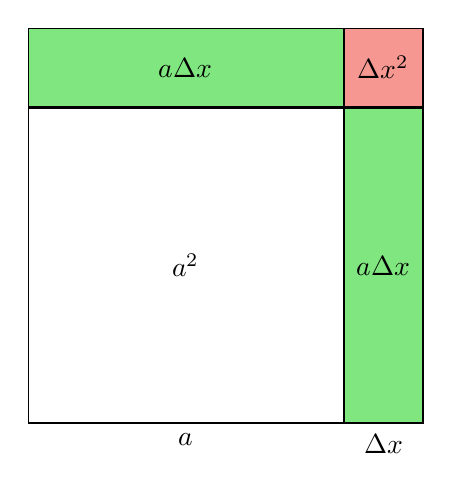
\begin{tikzpicture}
% \draw (0,0) node[below] {$a$} rectangle (4,4) node[midway] {$a^2$};
% \draw [fill=orange] (0,4) rectangle (4,5) node[midway] {$a\Delta x$};
% \draw [fill=orange] (4,0) rectangle (5,4) node[midway] {$a\Delta x$};
% \draw [fill=orange] (4,4) rectangle (5,5) node[midway] {$\Delta x^2$};
\node (A) [rectangle, draw, minimum width=4cm, minimum height=4cm, label={[anchor=north]south:$a$}] at (0,0) {$a^2$};
\node (B) [anchor=south, rectangle, draw, fill=color3!50, minimum width=4cm, minimum height=1cm] at (A.north) {$a\Delta x$};
\node (C) [anchor=west, rectangle, draw, fill=color3!50, minimum width=1cm, minimum height=4cm, label={[anchor=north]south:$\Delta x$}] at (A.east) {$a\Delta x$};
\node (D) [anchor=south, rectangle, draw, fill=color2!50, minimum width=1cm, minimum height=1cm] at (C.north) {$\Delta x^2$};
\end{tikzpicture}
}}
		\mode<presentation>{\resizebox{0.35\textwidth}{!}{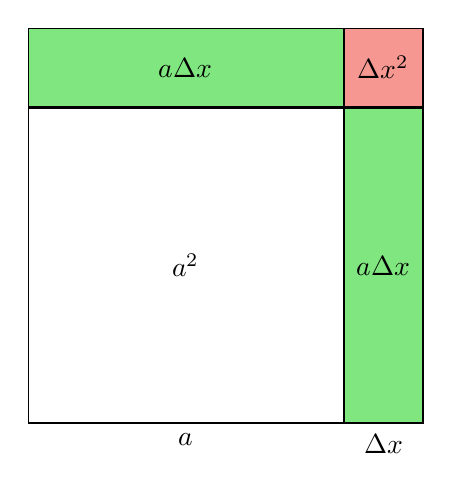
\begin{tikzpicture}
% \draw (0,0) node[below] {$a$} rectangle (4,4) node[midway] {$a^2$};
% \draw [fill=orange] (0,4) rectangle (4,5) node[midway] {$a\Delta x$};
% \draw [fill=orange] (4,0) rectangle (5,4) node[midway] {$a\Delta x$};
% \draw [fill=orange] (4,4) rectangle (5,5) node[midway] {$\Delta x^2$};
\node (A) [rectangle, draw, minimum width=4cm, minimum height=4cm, label={[anchor=north]south:$a$}] at (0,0) {$a^2$};
\node (B) [anchor=south, rectangle, draw, fill=color3!50, minimum width=4cm, minimum height=1cm] at (A.north) {$a\Delta x$};
\node (C) [anchor=west, rectangle, draw, fill=color3!50, minimum width=1cm, minimum height=4cm, label={[anchor=north]south:$\Delta x$}] at (A.east) {$a\Delta x$};
\node (D) [anchor=south, rectangle, draw, fill=color2!50, minimum width=1cm, minimum height=1cm] at (C.north) {$\Delta x^2$};
\end{tikzpicture}
}}
	\end{center}
\end{frame}


%---------------------------------------------------------------------slide----
\begin{frame}
	\frametitle{Approximating a function by a polynomial}
	Another useful application of the derivative is the approximation of functions by polynomials.
	
	Polynomials are functions easy to calculate (sums and products) with very good properties:
	\begin{itemize}
		\item Defined in all the real numbers.
		\item Continuous.
		\item Differentiable of all orders with continuous derivatives.
	\end{itemize}
	
	\begin{block}{Goal}
		Approximate a function $f(x)$ by a polynomial $p(x)$ near a point $x=a$.
	\end{block}
\end{frame}


%---------------------------------------------------------------------slide----
\begin{frame}
	\frametitle{Approximating a function by a polynomial of order 0}
	A polynomial of degree 0 has equation
	\[
		p(x) = c_0,
	\]
	where $c_0$ is a constant.
	
	As the polynomial should coincide with the function $f$ at $a$, it must satisfy
	\[p(a) = c_0 = f(a).\]
	
	Therefore, the polynomial of degree 0 that best approximates $f$ near $a$ is
	\[p(x) = f(a).\]
\end{frame}


%---------------------------------------------------------------------slide----
\begin{frame}
	\frametitle{Approximating a function by a polynomial of order 0}
	\begin{center}
		\tikzsetnextfilename{derivatives_1_variable/approximation_polynomial_0}
		% Author: Alfredo Sánchez Alberca (asalber@ceu.es)
\begin{tikzpicture}
  \begin{axis}[
    gen2dfun, 
    xmin=0, xmax=4,
    ymin=0, ymax=4,
    xtick={2.5},
    xticklabel={$x_0$},
    ytick={1.5},
    yticklabels={$f(x_0)$}, 
    clip=false, 
    height=5cm,
  	]
    \addplot+[domain=0.5:3.6, smooth, name path=F] {2.7183^(x-2.5)+0.5} node[anchor=south west] {$f(x)$};
    \coordinate (A) at (2.5,1.5);
    \fill (A) circle (1.2pt);
    \draw[gray, dotted] (A) -- (A|-O);
    \draw[gray, dotted] (A) -- (A-|O);
    \addplot+[domain=0.5:3.6, smooth, name path=P, visible on=<2->] {1.5} node[anchor=west] {$p^0=f(x_0)$};
    \coordinate (B) at (3.5,3.2183);
    \draw<3->[gray, very thin] (3.5,0.06) -- (3.5,-0.06);
    \node<3-> at (3.5,-0.25) {$x_1$};
    \draw<3->[gray, very thin] (-0.06,3.2183) -- (0.06,3.2183);
    \node<3-> at (-0.25,3.2183) {$x_1$};
    \draw<3->[gray, dotted] (B) -- (B|-O);
    \draw<3->[gray, dotted] (B) -- (B-|O);
    \draw[|-|, visible on=<4->] (B) -- (B|-A) node[anchor=west, pos=0.3] {Approximation error} node[anchor=west, midway] {$e^0(x_1)=f(x_1)-p^0(x_1)$};
  \end{axis};
\end{tikzpicture}

	\end{center}
\end{frame}


%---------------------------------------------------------------------slide----
\begin{frame}
	\frametitle{Approximating a function by a polynomial of order 1}
	A polynomial of degree 1 has equation
	\[
		p(x) = c_0+c_1x,
	\]
	but it can also be written as 
	\[
		p(x) = c_0+c_1(x-a).
	\]
	
	Among all the polynomials of degree 1, the one that best approximates $f$ near $a$ is that which meets the following conditions
	
	\begin{enumerate}
		\item $p$ and $f$ coincide at $a$: $p(a) = f(a)$,
		\item $p$ and $f$ have the same rate of change at $a$: $p'(a) = f'(a)$.
	\end{enumerate}
	
	The last condition guarantees that $p$ and $f$ have approximately the same tendency, but it requires the function $f$ to be differentiable at $a$.
\end{frame}


%---------------------------------------------------------------------slide----
\begin{frame}
	\frametitle{The tangent line: Best approximating polynomial of order 1}
	Imposing the previous conditions we have
	\begin{enumerate}
		\item $p(x)=c_0+c_1(x-a) \Rightarrow p(a)=c_0+c_1(a-a)=c_0=f(a)$,
		\item $p'(x)=c_1 \Rightarrow p'(a)=c_1=f'(a)$.
	\end{enumerate}
	
	Therefore, the polynomial of degree 1 that best approximates $f$ near $a$ is
	\[
		p(x) = f(a)+f '(a)(x-a),
	\]
	which turns out to be the tangent line to $f$ at $(a,f(a))$.
\end{frame}


%---------------------------------------------------------------------slide----
\begin{frame}
	\frametitle{Approximating a function by a polynomial of order 1}
	\begin{center}
		\tikzsetnextfilename{derivatives_1_variable/approximation_polynomial_1}
		% Author: Alfredo Sánchez Alberca (asalber@ceu.es)
\begin{tikzpicture}
  \begin{axis}[
    gen2dfun, 
    xmin=0, xmax=4,
    ymin=0, ymax=4,
    xtick={2.5},
    xticklabel={$x_0$},
    ytick={1.5},
    yticklabels={$f(x_0)$}, 
    clip=false, 
    height=5cm,
  	]
    \addplot+[domain=0.5:3.6, smooth, name path=F] {2.7183^(x-2.5)+0.5} node[anchor=south west] {$f(x)$};
    \coordinate (O);
    \coordinate (A) at (2.5,1.5);
    \fill (A) circle (1.2pt);
    \draw[gray, dotted] (A) -- (A|-O);
    \draw[gray, dotted] (A) -- (A-|O);
    \addplot+[domain=0.5:3.6, smooth, name path=P0, visible on=<2->] {1.5} node[anchor=west] {$p^0=f(x_0)$};
    \addplot+[domain=1:3.6, smooth, name path=P1, visible on=<3->] {x-1} node[anchor=west] {$p^1=f(x_0)+f'(x_0)(x-x_0)$};
    \coordinate (B) at (3.5,3.2183);
    \coordinate (C) at (3.5,2.5);
    \draw<4->[gray, very thin] (3.5,0.06) -- (3.5,-0.06);
    \node<4-> at (3.5,-0.25) {$x_1$};
    \draw<4->[gray, very thin] (-0.06,3.2183) -- (0.06,3.2183);
    \node<4->[anchor=east] at (-0.15,3.2183) {$f(x_1)$};
    \draw<4->[gray, very thin] (-0.06,2.5) -- (0.06,2.5);
    \node<4->[anchor=east] at (-0.15,2.5) {$p^1(x_1)$};
    \draw<4->[gray, dotted] (B) -- (B-|O);
    \draw<4->[gray, dotted] (B) -- (B|-O);
    \draw<4->[gray, dotted] (C) -- (C-|O);
    \draw[|-|, visible on=<5->] (B) -- (C) node[anchor=west, pos=0.1] {Approximation error} node[anchor=west, midway] {$e^1(x_1)=f(x_1)-p^1(x_1)$};
  \end{axis};
\end{tikzpicture}

	\end{center}
\end{frame}


%---------------------------------------------------------------------slide----
\begin{frame}
	\frametitle{Approximating a function by a polynomial of order 2}
	A polynomial of degree 2 is a parabola with equation
	\[
		p(x) = c_0+c_1x+c_2x^2,
	\]
	but it can also be written as
	\[
		p(x) = c_0+c_1(x-a)+c_2(x-a)^2.
	\]
	
	Among all the polynomials of degree 2, the one that best approximate $f(x)$ near $a$ is that which meets the following conditions
	\begin{enumerate}
		\item $p$ and $f$ coincide at $a$: $p(a) = f(a)$,
		\item $p$ and $f$ have the same rate of change at $a$: $p'(a) = f'(a)$.
		\item $p$ and $f$ have the same concavity at $a$: $p''(a)=f''(a)$.
	\end{enumerate}
	The last condition requires the function $f$ to be differentiable twice at $a$.
\end{frame}


%---------------------------------------------------------------------slide----
\begin{frame}
	\frametitle{Best approximating polynomial of order 2}
	Imposing the previous conditions we have
	\begin{enumerate}
		\item $p(x)=c_0+c_1(x-a) \Rightarrow p(a)=c_0+c_1(a-a)=c_0=f(a)$,
		\item $p'(x)=c_1 \Rightarrow p'(a)=c_1=f'(a)$.
		\item $p''(x)=2c_2 \Rightarrow p''(a)=2c_2=f''(a) \Rightarrow c_2=\frac{f''(a)}{2}$.
	\end{enumerate}
	
	Therefore, the polynomial of degree 2 that best approximates $f$ near $a$ is
	\[
		p(x) = f(a)+f'(a)(x-a)+\frac{f''(a)}{2}(x-a)^2.
	\]
\end{frame}


%---------------------------------------------------------------------slide----
\begin{frame}
	\frametitle{Approximating a function by a polynomial of order 2}
	\begin{center}
		\tikzsetnextfilename{derivatives_1_variable/approximation_polynomial_2}
		% Author: Alfredo Sánchez Alberca (asalber@ceu.es)
\begin{tikzpicture}[trim axis left, trim axis right]
  \begin{axis}[
    gen2dfun, 
    xmin=0, xmax=4,
    ymin=0, ymax=4,
    xtick={2.5},
    xticklabel={$a$},
    ytick={1.5},
    yticklabels={$f(a)$}, 
    clip=false, 
    height=5cm,
  	]
    \addplot+[domain=0.5:3.6, smooth, name path=F] {2.7183^(x-2.5)+0.5} node[anchor=south west] {$f(x)$};
    \coordinate (O);
    \coordinate (A) at (2.5,1.5);
    \fill (A) circle (1.2pt);
    \draw[gray, dotted] (A) -- (A|-O);
    \draw[gray, dotted] (A) -- (A-|O);
    \addplot+[domain=0.5:3.6, smooth, name path=P0, visible on=<2->] {1.5} node[anchor=west] {$p^0=f(a)$};
    \addplot+[domain=1:3.6, smooth, name path=P1, visible on=<3->] {x-1} node[anchor=west] {$p^1=f(a)+f'(a)(x-a)$};
    \addplot+[domain=0.5:3.6, smooth, name path=P1, visible on=<4->] {-1+x+(x-2.5)^2/2} node[anchor=west] {$p^2=f(a)+f'(a)(x-a)+\frac{f''(a)}{2}(x-a)^2$};
    \coordinate (B) at (3.5,3.2183);
    \coordinate (C) at (3.5,3);
    \draw<4->[gray, very thin] (3.5,0.05) -- (3.5,-0.05);
    \node<4-> at (3.5,-0.25) {$x$};
    \draw<4->[gray, very thin] (-0.06,3.2183) -- (0.06,3.2183);
    \node<4-> at (-0.25,3.2183) {$f(x)$};
    \draw<4->[gray, dotted] (B) -- (B|-O);
    \draw<4->[gray, dotted] (B) -- (B-|O);
    \draw[dashed, visible on=<5->] (B) -- (B|-A);
    \draw[decorate, decoration={brace, amplitude=4pt}, visible on=<5->] (B) -- (B|-A) node [pos=0.3, right, xshift=5pt] {Approximation error} node[midway, right, xshift=4pt] {$e^2(x)=f(x)-p^2(x)$};
  \end{axis};
\end{tikzpicture}

	\end{center}
\end{frame}


%---------------------------------------------------------------------slide----
\begin{frame}
	\frametitle{Approximating a function by a polynomial of order $n$}
	A polynomial of degree $n$ has equation
	\[
		p(x) = c_0+c_1x+c_2x^2+\cdots +c_nx^n,
	\]
	but it can also be written as
	\[
		p(x) = c_0+c_1(x-a)+c_2(x-a)^2+\cdots +c_n(x-a)^n.
	\]
	
	Among all the polynomials of degree $n$, the one that best approximate $f(x)$ near $a$ is that which meets the following $n+1$ conditions
	\begin{enumerate}
		\item $p(a) = f(a)$,
		\item $p'(a) = f'(a)$,
		\item $p''(a)=f''(a)$,
		\item[] $\cdots$
		\item[n+1.] $p^{(n)}(a)=f^{(n)}(a)$.
	\end{enumerate}
	
	\alert{Observe that these conditions require the function $f$ to be differentiable $n$ times at $a$.}
\end{frame}


%---------------------------------------------------------------------slide----
\begin{frame}
	\frametitle{Coefficients calculation for the best approximating polynomial of order $n$}
	The successive derivatives of $p$ are 
	\begin{align*}
		p(x)       & = c_0+c_1(x-a)+c_2(x-a)^2+\cdots +c_n(x-a)^n, \\
		p'(x)      & = c_1+2c_2(x-a)+\cdots +nc_n(x-a)^{n-1},      \\
		p''(x)     & = 2c_2+\cdots +n(n-1)c_n(x-a)^{n-2},          \\
		\vdots\ \
		\\
		p^{(n)}(x) & = n(n-1)(n-2)\cdots 1 c_n=n!c_n.              
	\end{align*}
	
	Imposing the previous conditions we have
	\begin{enumerate}
		\item $p(a) = c_0+c_1(a-a)+c_2(a-a)^2+\cdots +c_n(a-a)^n=c_0=f(a)$,
		\item $p'(a) = c_1+2c_2(a-a)+\cdots +nc_n(a-a)^{n-1}=c_1=f'(a)$,
		\item $p''(a) = 2c_2+\cdots +n(n-1)c_n(a-a)^{n-2}=2c_2=f''(a)\Rightarrow c_2=f''(a)/2$,
		\item[] $\cdots$
		\item[n+1.] $p^{(n)}(a)=n!c_n=f^{(n)}(a)=c_n=\frac{f^{(n)}(a)}{n!}$.
	\end{enumerate}
\end{frame}


%---------------------------------------------------------------------slide----
\begin{frame}
	\frametitle{Taylor polynomial of order $n$}
	\begin{definition}[Taylor polynomial]
		Given a function $f(x)$ differentiable $n$ times at $a$, the \emph{Taylor polynomial} of order $n$ of $f$ at $a$ is the polynomial with equation
		\begin{align*}
			p_{f,a}^n(x) & = f(a) + f'(a)(x-a) + \frac{f''(a)}{2}(x-a)^2 + \cdots + \frac{f^{(n)}(a)}{n!}(x-a)^n = \\ 
			             & = \sum_{i=0}^{n}\frac{f^{(i)}(a)}{i!}(x-a)^i.                                           
		\end{align*}
	\end{definition}
	
	The Taylor polynomial of order $n$ of $f$ at $a$ is the $n$th degree polynomial that best approximates $f$ near $a$, as is the only one that meets the previous conditions.
\end{frame} 


%---------------------------------------------------------------------slide----
\begin{frame}
	\frametitle{Taylor polynomial calculation}
	\framesubtitle{Example}
	Let us approximate the function $f(x)=\log x$ near the value $1$ by a polynomial of order $3$.
	
	The equation of the Taylor polynomial of order $3$ of $f$ at $a=1$ is
	\[
		p_{f,1}^3(x)=f(1)+f'(1)(x-1)+\frac{f''(1)}{2}(x-1)^2+\frac{f'''(1)}{3!}(x-1)^3.
	\]
	The derivatives of $f$ at $1$ up to order $3$ are
	\[
		\begin{array}{lll}
			f(x)=\log x   & \quad & f(1)=\log 1 =0,   \\
			f'(x)=1/x     &       & f'(1)=1/1=1,      \\
			f''(x)=-1/x^2 &       & f''(1)=-1/1^2=-1, \\
			f'''(x)=2/x^3 &       & f'''(1)=2/1^3=2.  
		\end{array}
	\]
	And substituting into the polynomial equation we get
	\[
		p_{f,1}^3(x)=0+1(x-1)+\frac{-1}{2}(x-1)^2+\frac{2}{3!}(x-1)^3= \frac{2}{3}x^3-\frac{3}{2}x^2+3x-\frac{11}{6}.
	\]
\end{frame}


%---------------------------------------------------------------------slide----
\begin{frame}
	\frametitle{Taylor polynomials of the logarithmic function}
	\begin{center}
		\tikzsetnextfilename{derivatives_1_variable/taylor_polynomials_logarithm}
		% Author: Alfredo Sánchez Alberca (asalber@ceu.es)
\begin{tikzpicture}
  \begin{axis}[
    2dfun, 
    xmin=0, xmax=4,
    ymin=-2, ymax=2,
    clip=false, 
    height=5cm,
  	]
    \addplot+[domain=0.2:2.8, smooth, samples=200] {ln(x)} node[anchor=west] {$f(x)=\log(x)$};
    \addplot+[domain=0.2:2.8, smooth, visible on=<2->] {x-1} node[anchor=west] {$p^1_{f,1}(x)=-1+x$};
    \addplot+[domain=0.2:2.8, smooth, visible on=<3->] {-1+x-(x-1)^2/2} node[anchor=west] {$p_{f,1}^2(x)=-1+x-\frac{1}{2}(x-1)^2$};
    \addplot+[domain=0.2:2.8, smooth, visible on=<4->] {-1+x-(x-1)^2/2+2/6*(x-1)^3} node[anchor=south west] {$p_{f,1}^3(x)=-1+x-\frac{1}{2}(x-1)^2+\frac{1}{3}(x-1)^3$};
    \coordinate (A) at (1,0);
    \fill (A) circle (1.2pt);
  \end{axis};
\end{tikzpicture}

	\end{center}
\end{frame}


%---------------------------------------------------------------------slide----
\begin{frame}
	\frametitle{Maclaurin polynomial of order $n$}
	The Taylor polynomial equation has a simpler form when the polynomial is calculated at $0$.
	This special case of Taylor polynomial at $0$ is known as the \emph{Maclaurin polynomial}.
	\begin{definition}[Maclaurin polynomial]
		Given a function $f(x)$ differentiable $n$ times at $0$, the \emph{Maclaurin polynomial} of order $n$ of $f$ is the polynomial with equation
		\begin{align*}
			p_{f,0}^n(x) & =f(0)+f'(0)x+\frac{f''(0)}{2}x^2+\cdots +\frac{f^{(n)}(0)}{n!}x^n = \\ &=\sum_{i=0}^{n}\frac{f^{(i)}(0)}{i!}x^i.
		\end{align*}
	\end{definition}
\end{frame}


%---------------------------------------------------------------------slide----
\begin{frame}
	\frametitle{Maclaurin polynomial calculation}
	\framesubtitle{Example}
	Let us approximate the function $f(x)=\sin x$ near the value $0$ by a polynomial of order $3$.
	
	The Maclaurin polynomial equation of order $3$ of $f$ is
	\[
		p_{f,0}^3(x)=f(0)+f'(0)x+\frac{f''(0)}{2}x^2+\frac{f'''(0)}{3!}x^3.
	\]
	The derivatives of $f$ at $0$ up to order $3$ are
	\[
		\begin{array}{lll}
			f(x)=\sin x     & \quad & f(0)=\sin 0 =0,     \\
			f'(x)=\cos x    &       & f'(0)=\cos 0=1,     \\
			f''(x)=-\sin x  &       & f''(0)=-\sin 0=0,   \\
			f'''(x)=-\cos x &       & f'''(0)=-\cos 0=-1. 
		\end{array}
	\]
	And substituting into the polynomial equation we get
	\[
		p_{f,0}^3(x)=0+1\cdot x+\frac{0}{2}x^2+\frac{-1}{3!}x^3= x-\frac{x^3}{6}.
	\]
\end{frame}


%---------------------------------------------------------------------slide----
\begin{frame}
	\frametitle{Maclaurin polynomial of the sine function}
	\begin{center}
		\tikzsetnextfilename{derivatives_1_variable/maclaurin_polynomials_sine}
		% Author: Alfredo Sánchez Alberca (asalber@ceu.es)
\begin{tikzpicture}[trim axis left, trim axis right]
  \begin{axis}[
    2dfun, 
    xmin=-3, xmax=3,
    ymin=-2, ymax=2,
    clip=false, 
    height=5cm,
  	]
    \addplot+[domain=-2.9:2.9, smooth, samples=200] {sin(deg(x))} node[anchor=west] {$f(x)=\sin(x)$};
    \addplot+[domain=-2:2, smooth, samples=200, visible on=<2->] {x} node[anchor=west] {$p^1_{f,0}(x)=x$};
    \addplot+[domain=-2.9:2.9, smooth, samples=200, visible on=<3->] {x-x^3/6} node[anchor=west] {$p_{f,0}^3(x)=x-\frac{1}{6}x^3$};
    \addplot+[domain=-2.9:2.9, smooth, samples=200, visible on=<4->] {x-x^3/6+x^5/120} node[anchor=west] {$p_{f,0}^5(x)=x-\frac{1}{6}x^3+\frac{1}{120}x^5$};
    \coordinate (A) at (0,0);
    \fill (A) circle (1.2pt);
  \end{axis};
\end{tikzpicture}

	\end{center}
\end{frame}


%---------------------------------------------------------------------slide----
\begin{frame}
	\frametitle{Maclaurin polynomials of elementary functions}
	\[
		\renewcommand{\arraystretch}{2.5}
		\begin{array}{cc}
			\toprule
			f(x)      & p_{f,0}^n(x)                                                                                                              \\
			\midrule
			\sin x    & \displaystyle x - \frac{x^3}{3!} + \frac{x^5}{5!} - \cdots + (-1)^k\frac{x^{2k-1}}{(2k-1)!} \mbox{ if $n=2k$ or $n=2k-1$} \\
			\cos x    & \displaystyle 1 - \frac{x^2}{2!} + \frac{x^4}{4!} - \cdots + (-1)^k\frac{x^{2k}}{(2k)!} \mbox{ if $n=2k$ or $n=2k+1$}     \\
			\arctan x & \displaystyle x - \frac{x^3}{3} + \frac{x^5}{5} - \cdots + (-1)^k\frac{x^{2k-1}}{(2k-1)} \mbox{ if $n=2k$ or $n=2k-1$}    \\
			e^x       & \displaystyle 1 + x + \frac{x^2}{2!} + \frac{x^3}{3!} + \cdots + \frac{x^n}{n!}                                           \\
			\log(1+x) & \displaystyle x - \frac{x^2}{2} + \frac{x^3}{3} - \cdots + (-1)^{n-1}\frac{x^n}{n}                                        \\
			\bottomrule
		\end{array}
	\]
\end{frame}


%---------------------------------------------------------------------slide----
\begin{frame}
	\frametitle{Taylor remainder and Taylor formula}
	Taylor polynomials allow to approximate a function in a neighborhood of a value $a$, but most of the times there is an error in the approximation.
	\begin{definition}[Taylor remainder]
		Given a function  $f(x)$ and its Taylor polynomial of order $n$ at $a$, $p_{f,a}^n(x)$, the \emph{Taylor remainder} of order $n$ of $f$ at $a$ is the difference between the function and the polynomial,
		\[
			r_{f,a}^n(x)=f(x)-p_{f,a}^n(x).
		\]
	\end{definition}
	
	The Taylor remainder measures the error in the approximation of $f(x)$ by the Taylor polynomial and allow us to express the function as the Taylor polynomial plus the Taylor remainder
	\[
		f(x)=p_{f,a}^n(x) + r_{f,a}^n(x).
	\]
	This expression is known as the \emph{Taylor formula} of order $n$ or $f$ at $a$. 
	
	It can be proved that
	\[
		\lim_{h\rightarrow 0}\frac{r_{f,a}^n(a+h)}{h^n}=0,
	\]
	which means that the remainder $r_{f,a}^n(a+h)$ is much smaller than $h^n$.
\end{frame}





% Author: Alfredo Sánchez Alberca (asalber@ceu.es)
% !TEX root = ../calculus_manual.tex
\section{Integrals}

\mode<presentation>{
%---------------------------------------------------------------------slide----
\begin{frame}
\frametitle{Integrals}
\tableofcontents[sectionstyle=show/hide,hideothersubsections]
\end{frame}
}


\subsection{Antiderivative of a function}
%---------------------------------------------------------------------slide----
\begin{frame}
\frametitle{Antiderivative of a function}
\begin{definition}[Antiderivative of a function]
Given a function $f(x)$, the function $F(X)$ is an \emph{antiderivative} or \emph{primitive function} of $f$ if it satisfies that $F'(x)=f(x)$ $\forall x \in \dom(f)$.
\end{definition}

\structure{\textbf{Example}} The function $F(x)=x^2$ is an antiderivative of the function $f(x)=2x$ as $F'(x)=2x$ on $\mathbb{R}$.

Roughly speaking, the calculus of antiderivatives is the reverse process of differentiation, and that is the reason for the name of antiderivative. 
\end{frame}


%---------------------------------------------------------------------slide----
\begin{frame}
\frametitle{Indefinite integral of a function}
As two functions that differs in a constant term have the same derivative, if $F(x)$ is an antiderivative of $f(x)$, so will be any function of the form $F(x)+k$ $\forall k \in \mathbb{R}$.
This means that, when a function has an antiderivative, it has an infinite number of antiderivatives. 

\begin{definition}[Indefinite integral]
The \emph{indefinite integral} of a function $f(x)$ is the set of all its antiderivatives; it is denoted by
\[
\int{f(x)}\,dx=F(x)+C
\]
where $F(x)$ is an antiderivative of $f(x)$ and $C$ is a constant.
\end{definition}

\structure{\textbf{Example}} The indefinite integral of the function $f(x)=2x$ is
\[\int 2x\, dx = x^2+C.\]
\end{frame}


%---------------------------------------------------------------------slide----
\begin{frame}
\frametitle{Interpretation of the integral}
We have seen in a previous chapter that the derivative of a function is the instantaneous rate of change of the function. 
Thus, if we know the instantaneous rate of change of the function at any point, we can compute the change of the function.

\structure{\textbf{Example}} What is the space covered by an free falling object?

Assume that the only force acting upon an object drop is gravity, with an acceleration of $9.8$ m/s$^2$. 
As acceleration is the the rate of change of the speed, that is constant at any moment, the antiderivative is the speed of the object, 
\[
v(t) = 9.8t  \mbox{ m/s}
\] 
And as the speed is the rate of change of the space covered by object during the fall, the antiderivative of the speed is the space covered by the object, 
\[
s(t) = \int 9.8t\, dt = 9,8\frac{t^2}{2}.
\]
Thus, for instance, after 2 seconds, the covered space is $s(2) = 9.8\frac{2^2}{2} = 19.6$ m.
\end{frame}


%---------------------------------------------------------------------slide----
\begin{frame}
\frametitle{Linearity of integration}
Given two integrable functions $f(x)$ and $g(x)$ and a constant $k \in \mathbb{R}$, it is satisfied that
\begin{enumerate}
\item $\int{(f(x)+g(x))}\,dx=\int{f(x)}\,dx+\int{g(x)}\,dx$,

\item $\int{kf(x)}\,dx=k\int{f(x)}\,dx$.
\end{enumerate}

This means that the integral of any linear combination of functions equals the same linear combination of the integrals of the functions.
\end{frame}


\subsection{Elementary integrals}
%---------------------------------------------------------------------slide----
\begin{frame}
\frametitle{Elementary integrals}
\begin{columns}
\begin{column}{0.5\textwidth}
\begin{itemize}
\item $\int a\,dx=ax+C$, with $a$ constant.
\item $\int x^n\,dx=\dfrac{x^{n+1}}{n+1}+C$ \quad if $n\neq -1$.
\item $\int \dfrac{1}{x}\, dx=\ln|x|+C$.
\item $\int e^x\,dx=e^x+C$.
\item $\int a^x\,dx=\dfrac{a^x}{\ln a}+C$.
\item $\int \sin x\, dx=-\cos x+C$.
\item $\int \cos x\, dx=\sin x+C$.
\item $\int \tan x\, dx=\ln|\sec x|+C$.
\item $\int \sec x\, dx = \ln|\sec x + \tan x|+C$.
\item $\int \csc x\, dx= \ln|\csc x-\cot x|+C$.
\end{itemize}
\end{column}
\begin{column}{0.5\textwidth}
\begin{itemize}
\item $\int \cot x \, dx= \ln|\sin x|+C$.
\item $\int \sec^2 x\, dx= \tan x+ C$.
\item $\int \csc^2 x\, dx= -\cot x+ C$.
\item $\int \sec x \tan x\, dx= \sec x+ C$.
\item $\int \csc x \cot x\, dx = -\csc x +C$.
\item $\int \dfrac{dx}{\sqrt{a^2-x^2}}=\arcsin\dfrac{x}{a}+C$.
\item $\int \dfrac{dx}{a^2+x^2}=\dfrac{1}{a}\arctan\dfrac{x}{a}+C$.
\item $\int \dfrac{dx}{x\sqrt{x^2-a^2}}=\dfrac{1}{a}\sec^{-1}\dfrac{x}{a}+C$.
\item $\int \dfrac{dx}{a^2-x^2}=\dfrac{1}{2a}\ln\left|\dfrac{x+a}{x-a}\right|+C$.
\end{itemize}
\end{column}
\end{columns}
\end{frame}


\subsection{Techniques of integration}
%---------------------------------------------------------------------slide----
\begin{frame}
\frametitle{Techniques of integration}
Unfortunately, unlike differential calculus, the is not a foolproof procedure to compute the antiderivative of a function.
However, there are some techniques that allow to integrate some types of functions. 
The most common methods of integration are
\begin{itemize}
\item Integration by parts
\item Integration by reduction
\item Integration by substitution
\item Integration of rational functions
\item Integration of trigonometric functions
\end{itemize}
\end{frame}


%---------------------------------------------------------------------slide----
\begin{frame}
\frametitle{Integration by parts}
Given two differentiable functions $u(x)$ and $v(x)$, from the rule for differentiating a product we can get
\[
\int{u(x)v'(x)}\,dx=u(x)v(x)-\int{u'(x)v(x)}\,dx,
\]
or, writing $u'(x)dx=du$ and $v'(x)dx=dv$,
\[
\int{u}\,dv=uv-\int{v}\,du.
\]
To apply this method we have to choose the functions $u$ and $dv$ in a way so that the final integral is easier to compute than the original one. 

\structure{\textbf{Example}} To integrate $\int{x \sin x}\,dx$ we have to choose $u=x$ and $dv=\sin x\, dx$, so $du=dx$ and $v=-\cos x$, getting
\[
\int{x \sin x}\,dx=-x\cos x-\int (-\cos x)\,dx = -x\cos x +\sin x.
\]
If we had chosen $u=\sin x$ and $dv=x\,dx$, we would have got a more difficult integral. 
\end{frame}



%---------------------------------------------------------------------slide----
\begin{frame}
\frametitle{Integration by reduction}
The reduction technique is used when we have to apply the integration by parts several times. 

If we want to compute the antiderivative $I_{n}$ that depends on a natural number $n$, the reduction formulas allow us to write $I_{n}$ as a function of $I_{n-1}$, that is, we have a recurrent relation
\[
\ I_{n}=f(I_{n-1},x,n)
\]
so by computing the first antiderivative $I_0$ we should be able to compute the others.

\structure{\textbf{Example}} To compute $I_{n}=\int{x^ne^x}\,dx$ applying integration by parts, we have to choose $u=x^n$ y $dv=e^x\,dx$, so $du=nx^{n-1}\,dx$ and $v=e^{x}$, getting
\[
\ I_{n}=\int{x^ne^x}\,dx=x^ne^x-n\int{x^{n-1}e^x}\,dx=x^ne^x-nI_{n-1}.
\]
Thus, for instance, for $n=3$ we have
\begin{align*}
\int x^3 e^x\, dx &= I_3 = x^3e^x-3I_2 = x^3e^x-3(x^2e^x-2I_1) = x^3e^x-3(x^2e^x-(xe^x-I_0) =\\
&= x^3e^x-3(x^2e^x-(xe^x-e^x) = e^x(x^3-3x^2+6x-6).
\end{align*}
\end{frame}


%---------------------------------------------------------------------slide----
\begin{frame}
\frametitle{Integration by substitution}
From the chain rule for differentiating the composition of two functions 
\[
f(g(x))' = f'(g(x))g'(x),
\]
we can make a variable change $u=g(x)$, so $du=g'(x)dx$, and get
\[
\int f'(g(x))g'(x)\, dx = \int f'(u)\, du = f(u)+C = f(g(x))+C.
\]

\structure{\textbf{Example}} To compute the integral of $\int{\dfrac{1}{x\log x}}\, dx$ we can make the substitution 
$u=\log x$, so $du=\frac{1}{x}dx$, and we have
\[
\int \frac{dx}{x\log x}=\int \frac{1}{\log x}\frac{1}{x}\,dx = \int \frac{1}{u}\,du = \log |u|+ C.
\]
Finally, undoing the substitution we get 
\[
\int \frac{1}{x\log x}\,dx= \log |\log x| + C.
\]
\end{frame}


%---------------------------------------------------------------------slide----
\begin{frame}
\frametitle{Integration of rational functions}
\framesubtitle{Partial fractions decomposition}
A rational function can be written as the sum of a polynomial (with an immediate antiderivative) plus a proper rational function, that is, a rational function in which the degree of the numerator is less than the degree of the denominator. 

On the other hand, depending of the factorization of the denominator, a proper rational function can be expressed as a sum of simpler fractions of the following types

\begin{itemize}
\item Denominator with a single linear factor: $\dfrac{A}{(x-a)}$
\item Denominator with a linear factor repeated $n$ times : $\dfrac{A}{(x-a)^{n}}$
\item Denominator with a single quadratic factor: $\dfrac{Ax+B}{x^2+cx+d}$
\item Denominator with a quadratic factor repeated $n$ times: $\dfrac{Ax+B}{(x^2+cx+d)^n}$
\end{itemize}
\end{frame}


%---------------------------------------------------------------------slide----
\begin{frame}
\frametitle{Integration of rational functions}
\framesubtitle{Antiderivatives of partial fractions}
Using the linearity of integration, we can compute the antiderivative of a rational function from the antiderivative of these partial fractions
\begin{align*}
\int \frac{A}{x-a}\,dx &= A\log|x-a|+C,\\
\int \frac{A}{(x-a)^n}\,dx &= \frac{-A}{(n-1)(x-a)^{n-1}}+C \textrm{ si $n\neq 1$}.\\
\int \frac{Ax+B}{x^2+cx+d} &= \frac{A}{2}\log|x^2+cx+d|+\frac{2B-Ac}{\sqrt{4d-c^2}}\arctan \frac{2x+c}{\sqrt{4d-c^2}}+C.
\end{align*}
\end{frame}


%---------------------------------------------------------------------slide----
\begin{frame}[allowframebreaks]
\frametitle{Integration of rational functions}
\framesubtitle{Example of denominator with linear factors}
Consider the function $f(x)=\dfrac{x^2+3x-5}{x^3-3x+2}$. 

The factorization of the denominator is $x^3-3x+2=(x-1)^2(x+2)$; it has a single linear factor $(x+2)$ and a linear factor $(x-1)$, repeated two times.
In this case the decomposition in partial fractions is:
\begin{align*}
\frac{x^2+3x-5}{x^3-3x+2}&=\frac{A}{x-1}+\frac{B}{(x-1)^2}+\frac{C}{x+2} = \\ &= \frac{A(x-1)(x+2)+ B(x+2)+C(x-1)^2}{(x-1)^2(x+2)} = \\ &= \frac{(A+C)x^2+(A+B-2C)x+(-2A+2B+C)}{(x-1)^2(x+2)}
\end{align*}
and equating the numerators we get $A=16/9$, $B=-1/3$ and $C=-7/9$, so
\[
\frac{x^2+3x-5}{x^3-3x+2}= \frac{16/9}{x-1}+\frac{-1/3}{(x-1)^2}+\frac{-7/9}{x+2}.
\]
Finally, integrating each partial fraction we have 
\begin{align*}
\int \frac{x^2+3x-5}{x^3-3x+2}\, dx &= \int \frac{16/9}{x-1}\,dx+\int \frac{-1/3}{(x-1)^2}\,dx+\int \frac{-7/9}{x+2}\,dx = \\ &=
\frac{16}{9}\int\frac{1}{x-1}\,dx-\frac{1}{3}\int(x-1)^{-2}\,dx- \frac{7}{9}\int \frac{1}{x+2}\,dx = \\
&= \frac{16}{9}\ln|x-1|+\frac{1}{3(x-1)}-\frac{7}{9}\ln|x+2|+C.
\end{align*}
\end{frame}


%---------------------------------------------------------------------slide----
\begin{frame}
\frametitle{Integration of rational functions}
\framesubtitle{Example of denominator with simple quadratic factors}
Consider the function $f(x)=\dfrac{x+1}{x^2-4x+8}$. 

In this case the denominator cannot be factorised as a product of linear factors, but we can write
\[
x^2-4x+8 = (x-2)^2+4,
\]
so
\begin{align*}
\int \dfrac{x+1}{x^2-4x+8}\, dx &= \int \dfrac{x-2+3}{(x-2)^2+4}\,dx = \\
&= \int \dfrac{x-2}{(x-2)^2+4}\,dx + \int \dfrac{3}{(x-2)^2+4}\,dx = \\
&= \frac{1}{2}\ln|(x-2)^2+4| + \dfrac{3}{2}\arctan\left(\frac{x-2}{2}\right)+C.
\end{align*}
\end{frame}


%---------------------------------------------------------------------slide----
\begin{frame}
\frametitle{Integration of trigonometric functions}
\framesubtitle{Integration of $\sin^n x\cos^m x$ with $n$ or $m$ odd}
If $f(x)=\sin^n x\cos^m x$ with $n$ or $m$ odd, then we can make the substitution $t=\sin x$ or
$t=\cos x$, to convert the function into a polynomial.

\structure{\textbf{Example}}
\[
\int \sin^2 x\cos^3 x\, dx = \int \sin^2 x\cos^2 x\cos x\, dx = \int \sin^2 x(1-\sin^2 x)\cos x\, dx,
\]
and making the substitution $t=\sin x$, so $dt = \cos x dx$, we have
\[
\int \sin^2 x(1-\sin^2 x)\cos x\, dx = \int t^2(1-t^2)\, dt = \int t^2-t^4 \, dt = \frac{t^3}{3}-\frac{t^5}{5}+C.
\]
Finally, undoing the substitution we have
\[
\int \sin^2 x\cos^3 x\, dx = \frac{\sin^3 x}{3}-\frac{\sin^5 x}{5}+C.
\]
\end{frame}


%---------------------------------------------------------------------slide----
\begin{frame}
\frametitle{Integration of trigonometric functions}
\framesubtitle{Integration of $\sin^n x\cos^m x$ with $n$ and $m$ even}
If $f(x)=\sin^n x\cos^m x$ with $n$ and $m$ even, then we can make the following substitutions to simplify the integration 
\begin{align*}
\sin^2 x &= \frac{1}{2}(1-\cos(2x))\\
\cos^2 x &= \frac{1}{2}(1+\cos(2x))\\
\sin x\cos x &= \frac{1}{2}\sin(2x)
\end{align*}

\structure{\textbf{Example}}
\begin{align*}
\int \sin^2 x\cos^4 x\, dx &= \int (\sin x\cos x)^2\cos^2 x\, dx = \int \left(\frac{1}{2}\sin(2x)\right)^2\frac{1}{2}(1+\cos(2x))\,dx =\\
&= \frac{1}{8}\int \sin^2(2x)\,dx+\frac{1}{8}\int \sin^2(2x) \cos(2x)\,dx,
\end{align*}
the first integral is of the same type and the second one of the previous type, so
\[
\int \sin^2 x\cos^4 x\, dx = \frac{1}{32}x-\frac{1}{32}\sin(2x)+\frac{1}{24}\sin^3(2x).
\] 
\end{frame}


%---------------------------------------------------------------------slide----
\begin{frame}
\frametitle{Integration of trigonometric functions}
\framesubtitle{Products of sines and cosines}
The equalities 
\begin{align*}
\sin x\cos y &= \frac{1}{2}(\sin(x-y)+\sin(x+y))\\
\sin x\sin y &= \frac{1}{2}(\cos(x-y)-\cos(x+y))\\
\cos x\cos y &= \frac{1}{2}(\cos(x-y)+\cos(x+y))
\end{align*}
transform products in sums, simplifying the integration 

\structure{\textbf{Example}}
\begin{align*}
\int \sin x\cos 2x\, dx &= \int \frac{1}{2}(\sin(x-2x)+\sin(x+2x))\,dx = \\
&= \frac{1}{2}\int \sin (-x)\,dx +\frac{1}{2}\int \sin 3x\,dx = \\
&= \frac{1}{2}\cos(-x)- \frac{1}{6}\cos 3x +C.
\end{align*}
\end{frame}


%---------------------------------------------------------------------slide----
\begin{frame}
\frametitle{Integration of trigonometric functions}
\framesubtitle{Rational functions of sines and cosines}
If $f(x,y)$ is a rational function then the function $f(\sin x,\cos x)$ can be transformed in an rational function of  
$t$ with the following substitutions
\[
\tan \frac{x}{2}=t \quad \sin x=\frac{2t}{1+t^2} \quad \cos x = \frac{1-t^2}{1+t^2} \quad dx = \frac{2}{1+t^2}dt. 
\]

\structure{\textbf{Example}}
\[
\int \frac{1}{\sin x}\,dx = \int \frac{1}{\frac{2t}{1+t^2}}\frac{2}{1+t^2}\,dt = \int \frac{1}{t}\,dt = \log|t|+C =
\log|\tan\frac{x}{2}|+C.
\]
\end{frame}



\subsection{Definite integral}
%---------------------------------------------------------------------slide----
\begin{frame}
\frametitle{Definite integral}
\begin{definition}[Definite integral]
Let $f(x)$ be a function which is continuous on an interval $[a, b]$.
Divide this interval into $n$ subintervals of equal width $\Delta x$ and choose an arbitrary point $x_i$ from each interval.
The \emph{definite integral} of $f$ from $a$ to $b$ is defined to be the limit
\[
\int_a^b f(x)\,dx = \lim_{n\rightarrow \infty}\sum_{i=1}^n f(x_i)\Delta x. 
\]
\end{definition}

\begin{center}
\tikzsetnextfilename{integrals/riemann_sums}
\mode<article>{% Author: Alfredo Sánchez Alberca (asalber@ceu.es)
\begin{tikzpicture}[/pgf/declare function={f=x^3-6*x^2+11*x-3;}, trim axis left, trim axis right]
\begin{axis}[
	gen2dfun,
	xmin=0, xmax=4,
	ymin=0, ymax=4,
	xtick={1,3},
	xticklabels={$a$,$b$},
	ytick={},
	yticklabels={},
    clip=false,
    width=4cm,
	]
	\addplot+[domain=0.7:3.3, samples=100, smooth, name path=F] {f} node[anchor=south] {$f(x)$};
	\draw[decorate, decoration={brace, amplitude=4pt}] (1,0) -- (1,3) node [midway, left, xshift=-2pt] {$f(x_i)$};
	\addplot[ybar interval, color1, fill=color1, opacity=0.3, domain=1:3, samples=5] {f};
%	\draw[decorate, decoration={brace, amplitude=4pt}] (1,0) -- (1,3) node [midway, left, xshift=-2pt] {$f(x)$};
	\draw[decorate, decoration={brace, amplitude=3pt, mirror}] (1,0) -- (1.5,0) node [midway, below, yshift=-2pt] {$\Delta x$};
%	\node at (2,1.5) {$\displaystyle \int_a^b f(x)\,dx$}; 
%	\path[name path=axis] (axis cs:1,0) -- (axis cs:3,0);
%    \addplot [thick, color=color1, fill=color1, fill opacity=0.3] fill between[of=F and axis, soft clip={domain=1:3},];
\end{axis}
\end{tikzpicture}
}
\mode<presentation>{% Author: Alfredo Sánchez Alberca (asalber@ceu.es)
\begin{tikzpicture}[/pgf/declare function={f=x^3-6*x^2+11*x-3;}, trim axis left, trim axis right]
\begin{axis}[
	gen2dfun,
	xmin=0, xmax=4,
	ymin=0, ymax=4,
	xtick={1,3},
	xticklabels={$a$,$b$},
	ytick={},
	yticklabels={},
    clip=false,
    width=4cm,
    height=3cm,
	]
	\addplot+[domain=0.7:3.3, samples=100, smooth, name path=F] {f} node[anchor=south] {$f(x)$};
	\foreach \x in {2,...,10}{
		\only<\x>{\addplot[ybar interval, fill=color1, opacity=0.3, domain=1:3, samples=\x] {f};}
	 	\pgfmathsetmacro{\coor}{1+2/(\x-1)}
     	\edef\temp{\noexpand\draw[decorate, decoration={brace, amplitude=3pt, mirror}, visible on=<\x>] (1,0) -- (\coor,0) node [midway, below, yshift=-2pt] {$\Delta x$};}
    	\temp
	}
	\draw[decorate, decoration={brace, amplitude=4pt}, visible on=<2-10>] (1,0) -- (1,3) node [midway, left, xshift=-2pt] {$f(x_i)$};
	\only<11>{\addplot[ybar interval, color1, fill=color1, opacity=0.3, domain=1:3, samples=50] {f};}
	\draw[decorate, decoration={brace, amplitude=4pt}, visible on=<11>] (1,0) -- (1,3) node [midway, left, xshift=-2pt] {$f(x)$};
	\node[below, visible on=<11>] at (2,0) {$dx$};
	\node[visible on=<12->] at (2,1.5) {$\displaystyle \int_a^b f(x)\,dx$}; 
	\path[name path=axis] (axis cs:1,0) -- (axis cs:3,0);
    \addplot [thick, color=color1, fill=color1, fill opacity=0.3, visible on=<12->] fill between[of=F and axis, soft clip={domain=1:3},];
\end{axis}
\end{tikzpicture}
}
\end{center}
\end{frame}


%---------------------------------------------------------------------slide----
\begin{frame}
\frametitle{Definite integral}
\begin{theorem}[First fundamental theorem of Calculus]
If $f(x)$ is continuous on the interval $[a,b]$ and $F(x)$ is an antiderivative of $f$ on $[a,b]$, then
\[
\int_a^b f(x)\,dx = F(b)-F(a)
\]
\end{theorem}
\structure{\textbf{Example}}. Given the function $f(x)=x^2$, we have
\[
\int_1^2 x^2\,dx = \left[\frac{x^3}{3}\right]_1^2 = \frac{2^3}{3}-\frac{1^3}{3} = \frac{7}{3}.
\]
\end{frame}


%---------------------------------------------------------------------slide----
\begin{frame}
\frametitle{Properties of the definite integral}
Given two functions $f(x)$ and $g(x)$ integrable on $[a,b]$ and $k \in \mathbb{R}$ the following properties are satisfied:
\begin{itemize}
\item $\int_{a}^{b}(f(x)+g(x))\,dx=\int_{a}^{b}f(x)\,dx+\int_{a}^{b}g(x)\,dx$ (linearity)
\item $\int_{a}^{b}{kf(x)}\,dx=k\int_{a}^{b}{f(x)}\,dx$ (linearity)
\item $\int_{a}^{b}{f(x)\,dx} \leq \int_{a}^{b}{g(x)\,dx}$ si $f(x)\leq g(x)\ \forall x \in [a,b]$ (monotony)
\item $\int_{a}^{b}{f(x)\,dx} = \int_{a}^{c}{f(x)\,dx}+\int_{c}^{b}{f(x)\,dx}$ for any $c\in(a,b)$ (additivity)
\item $\int_a^b f(x)\,dx = -\int_b^a f(x)\,dx$
\end{itemize}
\end{frame}



\subsection{Area calculation}
%---------------------------------------------------------------------slide----
\begin{frame}
\frametitle{Area calculation}
\framesubtitle{Area between a positive function and the $x$ axis}
If $f(x)$ is an integrable function on the interval $[a,b]$ and $f(x)\geq 0\ \forall x\in[a,b]$, then the definite integral 
\[\int_a^b f(x)\,dx\]
measures the area between the graph of $f$ and the $x$ axis on the interval $[a,b]$.
\begin{center}
\tikzsetnextfilename{integrals/area_positive_function}
% Author: Alfredo Sánchez Alberca (asalber@ceu.es)
\begin{tikzpicture}[trim axis left, trim axis right]
  \begin{axis}[
    gen2dfun, 
    xmin=0, xmax=4,
    ymin=0, ymax=4,
    xtick={1,3},
    xticklabels={$a$, $b$},
    ytick={},
    yticklabels={},
    clip=false, 
    height=3.5cm,
  	]
    \addplot+[domain=0.7:3.3, smooth, name path=F] {x^3-6*x^2+11*x-3} node[anchor=south west] {$f(x)$};
    \path[name path=axis] (axis cs:1,0) -- (axis cs:3,0);
    \addplot [thick, color=color1, fill=color1, fill opacity=0.3] fill between[of=F and axis, soft clip={domain=1:3},];
    \node at (2,1.5) {$\displaystyle\int_a^b f(x)\,dx$};
    \coordinate (O) at (0,0);
    \coordinate (A) at (1,3);
    \coordinate (B) at (3,3);
    \draw[gray, dashed] (A) -- (A|-O);
    \draw[gray, dashed] (B) -- (B|-O);
  \end{axis};
\end{tikzpicture}

\end{center}
\end{frame}


%---------------------------------------------------------------------slide----
\begin{frame}
\frametitle{Area calculation}
\framesubtitle{Area between a negative function and the $x$ axis}
If $f(x)$ is an integrable function on the interval $[a,b]$ and $f(x)\leq 0\ \forall x\in[a,b]$, then the area between the graph of $f$ and the $x$ axis on the interval $[a,b]$ is
\[
-\int_a^b f(x)\,dx.
\]
\begin{center}
\tikzsetnextfilename{integrals/area_negative_function}
% Author: Alfredo Sánchez Alberca (asalber@ceu.es)
\begin{tikzpicture}[trim axis left, trim axis right]
  \begin{axis}[
    gen2dfun, 
    xmin=0, xmax=4,
    ymin=-4, ymax=0,
    enlargelimits=0.1,
    xtick={1,3},
    xticklabels={$a$, $b$},
    ytick={},
    yticklabels={},
    xticklabel style={above, yshift=2pt},
    clip=false, 
    height=3.5cm,
  	]
    \addplot+[domain=0.7:3.3, smooth, name path=F] {-x^3+6*x^2-11*x+3} node[anchor=north west] {$f(x)$};
    \path[name path=axis] (axis cs:1,0) -- (axis cs:3,0);
    \addplot [thick, color=color1, fill=color1, fill opacity=0.3] fill between[of=F and axis, soft clip={domain=1:3},];
    \node at (2,-1.5) {-$\displaystyle\int_a^b f(x)\,dx$};
    \coordinate (O) at (0,0);
    \coordinate (A) at (1,-3);
    \coordinate (B) at (3,-3);
    \draw[gray, dashed] (A) -- (A|-O);
    \draw[gray, dashed] (B) -- (B|-O);
  \end{axis};
\end{tikzpicture}

\end{center}
\end{frame}


%---------------------------------------------------------------------slide----
\begin{frame}
\frametitle{Area calculation}
\framesubtitle{Area between a function and the $x$ axis}
In general, if $f(x)$ is an integrable function on the interval $[a,b]$, no matter the sign of $f$ on $[a,b]$, the area between the graph of $f$ and the $x$ axis on the interval $[a,b]$ is
\[
\int_a^b |f(x)|\,dx.
\]
\begin{center}
\tikzsetnextfilename{integrals/area_function}
% Author: Alfredo Sánchez Alberca (asalber@ceu.es)
\begin{tikzpicture}[trim axis left, trim axis right]
  \begin{axis}[
    gen2dfun, 
    xmin=0, xmax=4,
    ymin=-2, ymax=3,
    xtick={1,3},
    xticklabels={$a$, $b$},
    ytick={},
    yticklabels={},
    clip=false, 
    height=3.5cm,
  	]
    \addplot+[domain=0.7:3.3, samples=100, smooth, name path=F] {-x^3+7*x^2-13*x+6} node[anchor=south west] {$f(x)$};
    \path[name path=axis] (axis cs:1,0) -- (axis cs:3,0);
    \addplot [thick, color=color1, fill=color1, fill opacity=0.3] fill between[of=F and axis, soft clip={domain=1:3},];
    \node at (1.5,1.5) {$\displaystyle\int_a^b |f(x)|\,dx$};
    \coordinate (O) at (0,0);
    \coordinate (A) at (1,-1);
    \coordinate (B) at (3,3);
    \draw[gray, dashed] (A) -- (A|-O);
    \draw[gray, dashed] (B) -- (B|-O);
  \end{axis};
\end{tikzpicture}

\end{center}
\end{frame}


%---------------------------------------------------------------------slide----
\begin{frame}
\frametitle{Area calculation}
\framesubtitle{Area between two functions}
If $f(x)$ and $g(x)$ are two integrable functions on the interval $[a,b]$, then the area between the graph of $f$ and $g$ on the interval $[a,b]$ is
\[
\int_{a}^{b}{|f(x)- g(x)|\,dx}.
\]

\begin{center}
\tikzsetnextfilename{integrals/area_between_functions}
% Author: Alfredo Sánchez Alberca (asalber@ceu.es)
\begin{tikzpicture}[trim axis left, trim axis right]
  \begin{axis}[
    gen2dfun, 
    xmin=0, xmax=4,
    ymin=0, ymax=5,
    enlargelimits=0.1,
    xtick={1,3},
    xticklabels={$a$, $b$},
    ytick={},
    yticklabels={},
    clip=false, 
    height=4cm,
  	]
    \addplot+[domain=0.7:3.3, samples=100, smooth, name path=F] {x^3-6*x^2+11*x-3} node[anchor=south west] {$f(x)$};
    \addplot+[domain=0.7:3.3, samples=100, smooth, name path=G] {-x^3+7*x^2-13*x+8} node[anchor=south west] {$g(x)$};
    \addplot [thick, color=color1, fill=color1, fill opacity=0.3] fill between[of=F and G, soft clip={domain=1:3},];
    \node[anchor=west] at (2,2) {-$\displaystyle\int_a^b |f(x)-g(x)|\,dx$};
    \draw[gray, dashed] (1,1) -- (1,3);
    \draw[gray, dashed] (3,3) -- (3,5);
  \end{axis};
\end{tikzpicture}

\end{center}
\end{frame}
%% Author: Alfredo Sánchez Alberca (asalber@ceu.es)
% !TEX root = ../calculus_manual.tex
\section{Ordinary Differential Equations}

\mode<presentation>{
%---------------------------------------------------------------------slide----
\begin{frame}
\frametitle{Ordinary Differential Equations}
\tableofcontents[sectionstyle=show/hide,hideothersubsections]
\end{frame}
}


\subsection{Ordinary Differential Equations}
%---------------------------------------------------------------------slide----
\begin{frame}
\frametitle{Ordinary Differential Equation}
Often in Physics, Chemistry, Biology, Geometry, etc there arise equations that relate a function with its derivative, or successive derivatives.

\begin{definition}[Ordinary differential equation]
An \emph{ordinary differential equation} (O.D.E.) is a equation that relates an independent variable $x$, a function $y(x)$ that depends on $x$, and the successive derivatives of $y$, $y',y'',\ldots,y^{(n)}$; it can be written as
\[
F(x, y, y', y'',\ldots, y^{(n)})=0.
\] 
The \emph{order} of a differential equation is the greatest order of the derivatives in the equation. 
\end{definition}
Thus, for instance, the equation $y'''+sen(x)y'=2x$ is a differential equation of order 3.
\end{frame}


%---------------------------------------------------------------------slide----
\begin{frame}
\frametitle{Deducing a differential equation}
To deduce a differential equation that explains a natural phenomenon is essential to understand what a derivative is and how to interpret it. 

\structure{\textbf{Example}} Newton's law of cooling states
\begin{center}
\begin{minipage}{0.8\textwidth}
\textit{``The rate of change of the temperature of a body in a surrounding medium is proportional to the difference between the temperature of the body $T$ and the temperature of the medium $T_a$.''}
\end{minipage}
\end{center}
The rate of change of the temperature is the derivative of temperature with respect to time $dT/dt$.
Thus, Newton's law of cooling can be explained by the differential equation
\[
\frac{dT}{dt}=k(T-T_a),
\]
where $k$ is a proportionality constant.
\end{frame}


%---------------------------------------------------------------------slide----
\begin{frame}
\frametitle{Solution of an ordinary differential equation}
\begin{definition}[Solution of an ordinary differential equation]
Given an ordinary differential equation $F(x,y,y',y'',\ldots,y^{(n})=0$, the function $y=f(x)$ is a \emph{solution of the ordinary differential equation} if it satisfies the equation, that is, if
\[
F(x,f(x), f'(x), f''(x),\ldots, f^{(n}(x))=0.
\]
The graph of a solution of the ordinary differential equation is known as \emph{integral curve}.
\end{definition}

Solving an ordinary differential equations consists on finding all its solutions in a given domain. 
For integral calculus is required. 

The same manner than the indefinite integral is a family of antiderivatives, that differ in a constant term, after integrating an ordinary differential equation we get a family of solutions that differ in a constant.
We can get particular solutions by giving values to this constant.
\end{frame}


%---------------------------------------------------------------------slide----
\begin{frame}
\frametitle{General solution of an ordinary differential equation}
\begin{definition}[General solution of an ordinary differential equation]
Given an ordinary differential equation $F(x,y,y',y'',\ldots,y^{(n})=0$ of order $n$, the \emph{general solution} of the differential equation is a family of functions 
\[y =f (x,C_1,\ldots,C_n),\] 
depending on $n$ constants, such that for any value of $C_1,\ldots,C_n$ we get a solution of the differential equation. 
\end{definition}

For every value of the constant we get \emph{particular solution} of the differential equation.
Thus, when a differential equation can be solved, it has infinite solutions.

Geometrically, the general solution of a differential equation corresponds to a family of integral curves of the differential equation.

Often, it is common to impose conditions to the solutions of a differential equation to reduce the number of solutions. 
In many cases, these conditions allow to determine the values of the constants in the general solution to get a particular solution.
\end{frame}


%---------------------------------------------------------------------slide----
\begin{frame}
\frametitle{First order differential equations}
In this chapter we are going to study first order differential equations
\[
F(x,y,y')=0.
\]

The general solution of a first order differential equation is
\[
y = f (x,C),
\]
so to get a particular solution from the general one, it is enough to set the value of the constant $C$, and for that we only need to impose one initial condition.

\begin{definition}[Initial value problem]
The group consisting of a first order differential equation and an initial condition is known as \emph{initial value problem}:
\[
\begin{cases}
F(x,y,y')=0, & \mbox{First order differential equation;} \\
y(x_0)=y_0, & \mbox{Initial condition.}
\end{cases}
\]
\end{definition}

Solving an initial value problem consists in finding a solution of the first order differential equation that satisfies the initial condition.
\end{frame}


%---------------------------------------------------------------------slide----
\begin{frame}
\frametitle{Solving an initial value problem}
\framesubtitle{Example}
Recall the first order differential equation of the Newton's law of cooling,
\[
\frac{dT}{dt}=k(T-T_a),
\]
where $T$ is the temperature of the body and $T_a$ is the temperature of the surrounding medium.

It is easy to check that the general solution of this equation is 
\[T(t) = Ce^{kt}+T_a.\]

If we impose the initial condition that the temperature of the body at the initial instant is $5$ ºC, that is, $T(0)=5$, we have
\[T(0) = Ce^{k\cdot0}+T_a = C+T_a = 5,\]
from where we get $C=5-T_a$, and this give us the particular solution
\[
T(t) = (5-T_a)e^{kt}+T_a.
\]
\end{frame}


%---------------------------------------------------------------------slide----
\begin{frame}
\frametitle{Integral curve of an initial value problem}
\framesubtitle{Example}
If we assume in the previous example that the temperature of the surrounding medium is $T_a=0$ ºC and the cooling constant of the body is $k=1$, the general solution of the differential equation is
\[T(t)=Ce^t,\]
that is a family of integral curves.
Among all of them, only the one that passes through the point $(0,5)$ corresponds to the particular solution of the previous initial value problem. 
\begin{center}
\tikzsetnextfilename{ordinary_differential_equations/integral_curves}
% Author: Alfredo Sánchez Alberca (asalber@ceu.es)
\begin{tikzpicture}[trim axis left, trim axis right]
  \begin{axis}[
    2dfun, 
    xmin=-1, xmax=1,
    ymin=0, ymax=10,
    xlabel={$t$},         
    ylabel={$T$},      
    clip=false, 
    height=3cm,
  	]
  	\foreach \c in {1,2,3,4,6}{
  	\edef\temp{\noexpand \addplot[domain=-1:0.5, samples=100, smooth, thick, color1] {exp(x)*\c} node[anchor=west] {$T(t)=\c e^t$};}
  	\temp
    }
    \addplot[domain=-1:0.5, samples=100, smooth, thick, color2] {5*exp(x)} node[anchor=west] {$T(t)=5e^t$};
    \fill (0,5) circle (1.2pt);
  \end{axis};
\end{tikzpicture}

\end{center}
\end{frame}


%---------------------------------------------------------------------slide----
\begin{frame}
\frametitle{Existence and uniqueness of solutions}
\begin{theorem}[Existence and uniqueness of solutions of a first order ODE]
Given an initial value problem 
\[
\begin{cases}
y'=F(x,y);\\
y(x_0)=y_0;
\end{cases}
\]
if $F(x,y(x))$ is a function continuous on an open interval around the point $(x_0,y_0)$, then a solution of the initial value problem exists. 
If, in addition, $\frac{\partial F}{\partial y}$ is continuous in an open interval around $(x_0,y_0)$, the solution is unique. 
\end{theorem}

Although this theorem guarantees the existence and uniqueness of a solution of a first order differential equation, it does not provide a method to compute it. 
In fact, there is not a general method to solve first order differential equations, but we will see how to solve some types:
\begin{itemize}
\item Separable differential equations
\item Homogeneous differential equations
\item Linear differential equations
\end{itemize}
\end{frame}



\subsection{Separable differential equations}
%---------------------------------------------------------------------slide----
\begin{frame}
\frametitle{Separable differential equations}
\begin{definition}[Separable differential equation]
A \emph{separable differential equation} is a first order differential equation that can be written as
\[y'g(y)=f(x),\]
or what is the same,
\[g(y)dy=f(x)dx,\]
so the different variables are on different sides of the equality (the variables are separated).
\end{definition}

The general solution for a separable differential equation comes after integrating both sides of the equation
\[\int g(y)\,dy = \int f(x)\,dx+C.\]
\end{frame}


%---------------------------------------------------------------------slide----
\begin{frame}
\frametitle{Solving a separable differential equation}
\framesubtitle{Example}
The differential equation of the Newton's law of cooling 
\[\frac{dT}{dt}=k(T-T_a),\]
is a separable differential equation since it can be written as
\[\frac{1}{T-T_a}dT=k\,dt.\]

Integrating both sides of the equation we have
\[
\int \frac{1}{T-T_a}\,dT=\int k\,dt\Leftrightarrow \log(T-T_a)=kt+C,
\]
and solving for $T$ we get the general solution of the equation 
\[
T(t)=e^{kt+C}+T_a=e^Ce^{kt}+T_a=Ce^{kt}+T_a,
\]
rewriting $C=e^C$ as an arbitrary constant.
\end{frame}



\subsection{Homogeneous differential equations}
%---------------------------------------------------------------------slide----
\begin{frame}
\frametitle{Homogeneous functions}
\begin{definition}[Homogeneous function]
A function $f(x,y)$ is \emph{homogeneous} of degree $n$, if it satisfies
\[f(kx,ky)= k^nf(x,y),\]
for any value $k\in \mathbb{R}$.
\end{definition}

In particular, a homogeneous function of degree $0$ always satisfies
\[f(kx,ky)=f(x,y).\]

Setting $k=1/x$ we have
\[
f(x,y)=f\left(\frac{1}{x}x,\frac{1}{x}y\right)=f\left(1,\frac{y}{x}\right)=g\left(\frac{y}{x}\right).
\]
This way, a homogeneous function of degree $0$ always can be written as a function of $u=y/x$:
\[f(x,y)=g\left(\frac{y}{x}\right)=g(u).\]
\end{frame}


%---------------------------------------------------------------------slide----
\begin{frame}
\frametitle{Homogeneous differential equations}
\begin{definition}[Homogeneous differential equation]
A \emph{homogeneous differential equation} is a first order differential equation that can be written as 
\[y'=f(x,y),\]
where $f(x,y)$ is a homogeneous function of degree $0$.
\end{definition}

We can solve a homogeneous differential equation by making the substitution
\[
u=\frac{y}{x}\Leftrightarrow y=ux,
\]
so the equation becomes
\[
u'x+u=f(u),
\]
that is a separable differential equation.

Once solved the separable differential equation, the substitution must be undone.
\end{frame}


%---------------------------------------------------------------------slide----
\begin{frame}
\frametitle{Solving a homogeneous differential equation}
\framesubtitle{Example}
Let us consider the following differential equation
\[
4x-3y+y'(2y-3x)=0.
\]

Rewriting the equation in this way
\[
y'=\frac{3y-4x}{2y-3x}
\]
we can easily check that it is a homogeneous differential equation.

To solve this equation we have to do the substitution $y=ux$, and we get
\[
u'x+u=\frac{3ux-4x}{2ux-3x}=\frac{3u-4}{2u-3}
\]
that is a separable differential equation.

Separating the variables we have
\[
u'x=\frac{3u-4}{2u-3}-u=\frac{-2u^2+6u-4}{2u-3}\Leftrightarrow \frac{2u-3}{-2u^2+6u-4}\,du=\frac{1}{x}\,dx.
\]
\end{frame}


%---------------------------------------------------------------------slide----
\begin{frame}
\frametitle{Solving a homogeneous differential equation}
\framesubtitle{Example}
Now, integrating both sides of the equation we have
\[
\renewcommand{\arraystretch}{2}
\begin{array}{c}
\displaystyle \int \frac{2u-3}{-2u^2+6u-4}\,du=\int \frac{1}{x}\,dx
\Leftrightarrow -\frac{1}{2}\log|u^2-3u+2|=\log|x|+C \Leftrightarrow\\
\Leftrightarrow \log|u^2-3u+2|=-2\log|x|-2C,
\end{array}
\]
then, applying the exponential function to both sides and simplifying we get the general solution 
\[
u^2-3u+2=e^{-2\log|x|-2C}=\frac{e^{-2C}}{e^{\log|x|^2}}=\frac{C}{x^2},
\]
rewriting the constant $K=e^{-2C}$.

Finally, undoing the initial substitution $u=y/x$, we arrive at the general solution of the homogeneous differential equation
\[
\left(\frac{y}{x}\right)^2-3\frac{y}{x}+2=\frac{K}{x^2}\Leftrightarrow y^2-3xy+2x^2=K.
\]
\end{frame}



\subsection{Linear differential equations}
%---------------------------------------------------------------------slide----
\begin{frame}
\frametitle{Linear differential equations}
\begin{definition}[Linear differential equation]
A \emph{linear differential equation} is a first order differential equation that can be written as
\[y'+g(x)y = h(x).\]
\end{definition}

To solve a linear differential equation we try to write the left side of the equation as the derivative of a product. 
For that we multiply both sides by a function $f(x)$, such that
\[f'(x)=g(x)f(x).\]
Thus, we get
\[
\begin{array}{c}
y'f(x)+g(x)f(x)y=h(x)f(x)\\
\Updownarrow\\
y'f(x)+f'(x)y=h(x)f(x)\\
\Updownarrow\\
\dfrac{d}{dx}(yf(x))=h(x)f(x)
\end{array}
\]
\end{frame}


%---------------------------------------------------------------------slide----
\begin{frame}
\frametitle{Solving a linear differential equation}
Integrating both sides of the previous equation we get the solution
\[
yf(x)=\int h(x)f(x)\,dx+C.
\]
On the other hand, the unique function that satisfies $f'(x)=g(x)f(x)$ is
\[
f(x)=e^{\int g(x)\,dx},
\]
so, substituting this function in the previous solution we arrive at the solution of the linear differential equation
\[
ye^{\int g(x)\,dx}=\int h(x) e^{\int g(x)\,dx}\,dx+C,
\]
or what is the same
\[
y=e^{-\int g(x)\,dx}\left(\int h(x)e^{\int g(x)\,dx}\,dx+C\right).
\]
\end{frame}


%---------------------------------------------------------------------slide----
\begin{frame}
\frametitle{Solving a linear differential equation}
\framesubtitle{Example}
If in the differential equation of the Newton's law of cooling the temperature of the surrounding medium is a function of time $T_a(t)$, then the differential equation 
\[
\frac{dT}{dt}=k(T-T_a(t)),
\]
is a linear differential equation since it can be written as
\[
T'-kT=-kT_a(t),
\]
where the independent term is $-kT_a(t)$ and the coefficient of $T$ is $-k$.

Substituting in the formula of the general solution of a linear differential equation we have
\[
y=e^{-\int -k\,dt}\left(\int -kT_a(t)e^{\int -k\,dt}\,dt+C\right)=
e^{kt}\left(-\int kT_a(t)e^{-kt}\,dt+C\right).
\]
\end{frame}


%---------------------------------------------------------------------slide----
\begin{frame}
\frametitle{Solving a linear differential equation}
\framesubtitle{Example}
In the particular case that $T_a(t)=t$, and the proportionality constant $k=1$, the general solution of the linear differential equation is
\[
y=e^{t}\left(-\int te^{-kt}\,dt+C\right)=e^t(e^{-t}(t+1)+C)=Ce^t+t+1.
\]
If, in addition, we know that the temperature of the body at time $t=0$ is $5$ ºC, that is, we have the initial condition $T(0)=5$, then we can compute the value of the constant $C$,
\[
y(0)=Ce^0+0+1=5 \Leftrightarrow C+1=5 \Leftrightarrow C=4,
\]
and we get the particular solution
\[
y(t)=4e^t+t+1.
\]
\end{frame}

%\section{Cálculo diferencial en varias variables}
%---------------------------------------------------------------------slide----
\begin{frame}
\frametitle{Cálculo diferencial en varias variables}
\tableofcontents[sectionstyle=show/hide,hideothersubsections]
\end{frame}


% ---------------------------------------------------------------------slide----
\begin{frame}
\frametitle{Generalization to curvilinear motion}
The notion of derivative as a velocity along a trajectory in the real line can be generalized to a trajectory in any euclidean space $\mathbb{R}^n$.

In case of a two dimensional space $\mathbb{R}^2$, if $f(t)$ describes the position of a moving object in the real plane at any time $t$, taking as reference the coordinates origin $O$ and the unitary vectors $\{\mathbf{i}=(1,0),\mathbf{j}=(0,1)\}$, we can represent the position of the moving object $P$ at every moment $t$ with a vector $\vec{OP}=x(t)\mathbf{i}+y(t)\mathbf{j}$, where the coordinates 
\[
\begin{cases}
x=x(t)\\
y=y(t)
\end{cases}
\quad
t\in \mbox{Dom}(f)
\]
are known as \emph{coordinate functions} of $f$; we write $f(t)=(x(t),y(t))$.

\begin{center}
\tikzsetnextfilename{derivatives_1_variable/curvilinear_motion}
\mode<article>{% Author: Alfredo Sánchez Alberca (asalber@ceu.es)
\begin{tikzpicture}
\draw (-5,1) -- (-3,1) node[midway, above=0.5] {Time};
\draw (-4,0.9) -- (-4,1.1) node[anchor=south] (A) {$t$};
\begin{axis}[
    gen2dfun, 
    xmin=-0.1, xmax=3,
    ymin=-0.1, ymax=3,
    axis equal=true,  
    xtick={1,2},
    xticklabels={$1$,$x(t)$},
    ytick={1,2.041471},
    yticklabels={$1$,$y(t)$}, 
    height=2cm,
    clip=false,
    ]
    \addplot+[domain=-0.2:3, smooth, name path=F] {sin(deg(x-1))+1.2};
    \coordinate (O) at (0,0);
    \coordinate (I) at (1,0);
    \coordinate (J) at (0,1);
    \draw [->, color1] (O) -- (I) node[above] {$\mathbf{i}$};
    \draw [->, color1] (O) -- (J) node[right] {$\mathbf{j}$};
    \coordinate (P) at (2,2.041471);
    \fill (P) circle (1.2pt) node[anchor=south west] (Plabel) {$P=f(t)$};
    \draw[gray, dotted] (P) -- (P|-O);
    \draw[gray, dotted] (P) -- (P-|O);
    \draw[->, color2] (O) -- (P);
\end{axis};
\node at (1.2,2.5) {Position};
\path [->, dashed] (A) edge[bend left=20] node[above] {$f$} (Plabel);
\end{tikzpicture}
}
\mode<presentation>{\scalebox{0.8}{% Author: Alfredo Sánchez Alberca (asalber@ceu.es)
\begin{tikzpicture}
\draw (-5,1) -- (-3,1) node[midway, above=0.5] {Time};
\draw (-4,0.9) -- (-4,1.1) node[anchor=south] (A) {$t$};
\begin{axis}[
    gen2dfun, 
    xmin=-0.1, xmax=3,
    ymin=-0.1, ymax=3,
    axis equal=true,  
    xtick={1,2},
    xticklabels={$1$,$x(t)$},
    ytick={1,2.041471},
    yticklabels={$1$,$y(t)$}, 
    height=2cm,
    clip=false,
    ]
    \addplot+[domain=-0.2:3, smooth, name path=F] {sin(deg(x-1))+1.2};
    \coordinate (O) at (0,0);
    \coordinate (I) at (1,0);
    \coordinate (J) at (0,1);
    \draw [->, color1] (O) -- (I) node[above] {$\mathbf{i}$};
    \draw [->, color1] (O) -- (J) node[right] {$\mathbf{j}$};
    \coordinate (P) at (2,2.041471);
    \fill (P) circle (1.2pt) node[anchor=south west] (Plabel) {$P=f(t)$};
    \draw[gray, dotted] (P) -- (P|-O);
    \draw[gray, dotted] (P) -- (P-|O);
    \draw[->, color2] (O) -- (P);
\end{axis};
\node at (1.2,2.5) {Position};
\path [->, dashed] (A) edge[bend left=20] node[above] {$f$} (Plabel);
\end{tikzpicture}
}}
\end{center}
\end{frame}


% ---------------------------------------------------------------------slide----
\begin{frame}
\frametitle{Velocity of a curvilinear motion in the plane}
In the context of a trajectory $f(t)=(x(t),y(t))$ in the real plane $\mathbb{R}^2$, the derivative of the function $f(t)$ at the moment $a$ is the vector
\[
\mathbf{v} = \lim_{\Delta t\rightarrow 0} \frac{f(a+\Delta t)-f(a)}{\Delta t},
\]
that is known, as long as the limit exists, as the \emph{velocity} of the trajectory $f$ at moment $a$.

As $f(t)=(x(t),y(t))$,
\begin{align*}
f'(a)&=\lim_{\Delta t\rightarrow 0} \frac{f(a+\Delta t)-f(a)}{\Delta t} = \lim_{\Delta t\rightarrow 0} \frac{(x(a+\Delta t),y(a+\Delta t))-(x(a),y(a))}{\Delta t} =\\
&=  \lim_{\Delta t\rightarrow 0} \left(\frac{x(a+\Delta t)-x(a)}{\Delta t},\frac{y(a+\Delta t)-y(a)}{\Delta t}\right) =\\
&= \left(\lim_{\Delta t\rightarrow 0}\frac{x(a+\Delta t)-x(a)}{\Delta t},\lim_{\Delta t\rightarrow 0}\frac{y(a+\Delta t)-y(a)}{\Delta t}\right) = (x'(a),y'(a)).
\end{align*}
Thus, 
\[
\mathbf{v} = x'(a)\mathbf{i}+y'(a)\mathbf{j}.
\]
\end{frame}


% ---------------------------------------------------------------------slide----
\begin{frame}
\frametitle{Velocity of a curvilinear motion in the plane}
\framesubtitle{Example}
Given the trajectory $f(t) = (\cos t,\sin t)$, $t\in \mathbb{R}$, whose image is the unit circumference centered in the coordinate origin, its coordinate functions are $x(t) = \cos t$, $y(t) = \sin t$, $t\in \mathbb{R}$, and its velocity is
\[
\mathbf{v}=f'(t)=(x'(t),y'(t))=(-\sin t, \cos t).
\]
In the moment $t=\pi/4$, the object is in position $f(\pi/4) = (\cos(\pi/4),\sin(\pi/4)) =(\sqrt{2}/2,\sqrt{2}/2)$
and it is moving with a velocity $\mathbf{v}=f'(\pi/4)=(-\sin(\pi/4),\cos(\pi/4))=(-\sqrt{2}/2,\sqrt{2}/2)$.
\begin{center}
\tikzsetnextfilename{derivatives_1_variable/circumference_trajectory}
\mode<article>{% Author: Alfredo Sánchez Alberca (asalber@ceu.es)
\begin{tikzpicture}
\begin{axis}[
    2dfun, 
    xmin=-1.5, xmax=1.5,
    ymin=-1.5, ymax=1.5,
    axis equal=true,  
    height=3cm,
    clip=false,
    ]
	\addplot+[domain=0:2*pi, samples=200, smooth]({cos(deg(x))},{sin(deg(x))});
	\coordinate (P) at (0.7071068,0.7071068); 
	\fill (P) circle (1.2pt) node [anchor=south west] {$P=f(\pi/4)$};
	\draw [->, color2] (P) -- (0,1.4142);
\end{axis};
\end{tikzpicture}
}
\mode<presentation>{\scalebox{0.8}{% Author: Alfredo Sánchez Alberca (asalber@ceu.es)
\begin{tikzpicture}
\begin{axis}[
    2dfun, 
    xmin=-1.5, xmax=1.5,
    ymin=-1.5, ymax=1.5,
    axis equal=true,  
    height=3cm,
    clip=false,
    ]
	\addplot+[domain=0:2*pi, samples=200, smooth]({cos(deg(x))},{sin(deg(x))});
	\coordinate (P) at (0.7071068,0.7071068); 
	\fill (P) circle (1.2pt) node [anchor=south west] {$P=f(\pi/4)$};
	\draw [->, color2] (P) -- (0,1.4142);
\end{axis};
\end{tikzpicture}
}}
\end{center}
Observe that the module of the velocity vector is always 1 as
$|\mathbf{v}|=\sqrt{(-\sin t)^2+(\cos t)^2}=1$.
\end{frame}



\subsection{Tangent line to a trajectory}
% ---------------------------------------------------------------------slide----
\begin{frame}
\frametitle{Tangent line to a trajectory in the plane}
\framesubtitle{Vectorial equation}
Given a trajectory $f(t)$ in the real plane, the vectors that are parallel to the velocity $\mathbf{v}$ at a moment $a$ are called \emph{tangent vectors} to the trajectory $f$ at the moment $a$, and the line passing through $P=f(a)$ directed by $\mathbf{v}$ is the tangent line to the graph of $f$ at the moment $a$.

\begin{definition}[Tangent line to a trajectory]
Given a trajectory $f(t)$ in the real plane $\mathbb{R}^2$, the \emph{tangent line} to to the graph of $f$ at $a$ is the line with equation
\begin{align*}
l:(x,y) &= f(a)+tf'(a) = (x(a),y(a))+t(x'(a),y'(a))\\
& = (x(a)+tx'(a),y(a)+ty'(a)).
\end{align*}
\end{definition}
\end{frame}


% ---------------------------------------------------------------------slide----
\begin{frame}
\frametitle{Tangent line to a trajectory in the plane}
\framesubtitle{Example}
We have seen that for the trajectory $f(t) = (\cos t,\sin t)$, $t\in \mathbb{R}$, whose image is the unit circumference centered at the coordinate origin, the object position at the moment $t=\pi/4$ is $f(\pi/4)=(\sqrt{2}/2,\sqrt{2}/2)$ and its velocity $\mathbf{v}=(-\sqrt{2}/2,\sqrt{2}/2)$. 
Thus the equation of the tangent line to $f$ at that moment is 
\[
l: (x,y) = f(\pi/4)+t\mathbf{v} =
\left(\frac{\sqrt{2}}{2},\frac{\sqrt{2}}{2}\right)+t\left(\frac{-\sqrt{2}}{2},\frac{\sqrt{2}}{2}\right) =
\left(\frac{\sqrt{2}}{2}-t\frac{\sqrt{2}}{2},\frac{\sqrt{2}}{2}+t\frac{\sqrt{2}}{2}\right).
\]
\end{frame}


% ---------------------------------------------------------------------slide----
\begin{frame}
\frametitle{Tangent line to a trajectory in the plane}
\framesubtitle{Cartesian and point-slope equations}
From the vectorial equation of the tangent to a trajectory $f(t)$ at the moment $t=a$ we can get the coordinate functions
\[
\begin{cases}
x=x(a)+tx'(a)\\
y=y(a)+ty'(a)
\end{cases}
\quad t\in \mathbb{R},
\]
and solving for $t$ and equalling both equations we get the \emph{Cartesian equation} of the tangent
\[
\frac{x-x(a)}{x'(a)}=\frac{y-y(a)}{y'(a)},
\]
if $x'(a)\neq 0$ and $y'(a)\neq 0$.

From this equation it is easy to get the \emph{point-slope equation} of the tangent
\[
y-y(a)=\frac{y'(a)}{x'(a)}(x-x(a)).
\]
\end{frame}


% ---------------------------------------------------------------------slide----
\begin{frame}
\frametitle{Tangent line to a trajectory in the plane}
\framesubtitle{Example of Cartesian and point-slope equations}
Using the vectorial equation of the tangent of the previous example
\[
l: (x,y)=\left(\frac{\sqrt{2}}{2}-t\frac{\sqrt{2}}{2},\frac{\sqrt{2}}{2}+t\frac{\sqrt{2}}{2}\right),
\]
its Cartesian equation is 
\[
\frac{x-\sqrt{2}/2}{-\sqrt{2}/2} = \frac{y-\sqrt{2}/2}{\sqrt{2}/2}
\]
and the point-slope equation is 
\[
y-\sqrt{2}/2 = \frac{-\sqrt{2}/2}{\sqrt{2}/2}(x-\sqrt{2}/2) \Rightarrow y=-x+\sqrt{2}.
\]
\end{frame}


% ---------------------------------------------------------------------slide----
\begin{frame}
\frametitle{Normal line to a trajectory in the plane}
We have seen that the tangent line to a trajectory $f(t)$ at $a$ is the line passing through the point 
$P=f(a)$ directed by the velocity vector $\mathbf{v}=f'(a)=(x'(a),y'(a))$. 
If we take as direction vector a vector orthogonal to $\mathbf{v}$, we get another line that is known as \emph{normal line} to the graph of $f$ at moment $a$.
\begin{definition}[Normal line to a trajectory]
Given a trajectory $f(t)$ in the real plane $\mathbb{R}^2$, the \emph{normal line} to the graph of $f$ at moment $t=a$ is the line with equation
\[
l: (x,y)=(x(a),y(a))+t(y'(a),-x'(a)) = (x(a)+ty'(a),y(a)-tx'(a)).
\]
\end{definition}
The Cartesian equation is 
\[
\frac{x-x(a)}{y'(a)} = \frac{y-y(a)}{-x'(a)},
\]
and the point-slope equation is
\[
y-y(a) = \frac{-x'(a)}{y'(a)}(x-x(a)).
\]
The normal line is always perpendicular to the tangent line as their direction vectors are orthogonal. 
\end{frame}


% ---------------------------------------------------------------------slide----
\begin{frame}
\frametitle{Normal line to a trajectory in the plane}
\framesubtitle{Example}
Considering again the trajectory of the unit circumference $f(t) = (\cos t,\sin t)$, $t\in \mathbb{R}$, the normal line to the graph of $f$ at moment $t=\pi/4$ is
\begin{align*}
l: (x,y)&=(\cos(\pi/2),\sin(\pi/2))+t(\cos(\pi/2),\sin(\pi/2)) =\\
&= \left(\frac{\sqrt{2}}{2},\frac{\sqrt{2}}{2}\right)+t\left(\frac{\sqrt{2}}{2},\frac{\sqrt{2}}{2}\right)
=\left(\frac{\sqrt{2}}{2}+t\frac{\sqrt{2}}{2},\frac{\sqrt{2}}{2}+t\frac{\sqrt{2}}{2}\right),
\end{align*}
the Cartesian equation is 
\[
\frac{x-\sqrt{2}/2}{\sqrt{2}/2} = \frac{y-\sqrt{2}/2}{\sqrt{2}/2},
\]
and the point-slope equation is 
\[
y-\sqrt{2}/2 = \frac{\sqrt{2}/2}{\sqrt{2}/2}(x-\sqrt{2}/2) \Rightarrow y=x.
\]
% \begin{center}
% \scalebox{0.8}{\input{img/calculo_diferencial_1_variable/circunferencia_tangente_normal}}
% \end{center}
\end{frame}


% ---------------------------------------------------------------------slide----
\begin{frame}
\frametitle{Tangent and normal lines to a function}
A particular case of tangent and normal lines to a trajectory are the tangent and normal lines to a function of one real variable. 
For every function $y=f(x)$, the trajectory that trace its graph is
\[
g(x) = (x,f(x))  \quad x\in \mathbb{R},
\]
and its velocity is 
\[
g'(x) = (1,f'(x)),
\]
so that the tangent line to $g$ at the moment $a$ is
\[
\frac{x-a}{1} = \frac{y-f(a)}{f'(a)} \Rightarrow y-f(a) = f'(a)(x-a),
\]
and the normal line is 
\[
\frac{x-a}{f'(a)} = \frac{y-f(a)}{-1} \Rightarrow y-f(a) = \frac{-1}{f'(a)}(x-a),
\]
\end{frame}


% ---------------------------------------------------------------------slide----
\begin{frame}
\frametitle{Tangent and normal lines to a function}
\framesubtitle{Example}
Given the function $y=x^2$, the trajectory that traces its graph is $g(x)=(x,x^2)$ and its velocity is 
$g'(x)=(1,2x)$. At the moment $x=1$ the trajectory passes through the point $(1,1)$ with a velocity $(1,2)$.
Thus, the tangent line at that moment is 
\[
\frac{x-1}{1} = \frac{y-1}{2} \Rightarrow y-1 = 2(x-1) \Rightarrow y = 2x-1,
\]
and the normal line is 
\[
\frac{x-1}{2} = \frac{y-1}{-1} \Rightarrow y-1 = \frac{-1}{2}(x-1) \Rightarrow y = \frac{-x}{2}+\frac{3}{2}.
\]
\begin{center}
\tikzsetnextfilename{derivatives_1_variable/parable_tangent_normal}
% Author: Alfredo Sánchez Alberca (asalber@ceu.es)
\begin{tikzpicture}
  \begin{axis}[
    2dfun, 
    xmin=-2, xmax=2,
    ymin=-0.2, ymax=3,
    axis equal=true,
    clip=false,  
    height=2cm,
    ]
    \addplot+[domain=-2:2] {x^2} node[anchor=south] {$f(x)=x^2$};
    \addplot+[domain=0.2:2] {2*x-1} node[anchor=west] {Tangent $y=2x-1$};
    \addplot+[domain=-2:2] {-x/2+3/2} node[anchor=west] {Normal $y=-\frac{x}{2}+\frac{3}{2}$};
    \coordinate (A) at (1,1);
    \fill (A) circle (1.2pt);
  \end{axis}
\end{tikzpicture}

\end{center}
\end{frame}


% ---------------------------------------------------------------------slide----
\begin{frame}
\frametitle{Tangent line to a trajectory in the space}
The concept of tangent line to a trajectory can be easily extended from the real plane to the three-dimensional space $\mathbb{R}^3$.

If $f(t)=(x(t),y(t),z(t))$, $t\in \mathbb{R}$, is a trajectory in the real space $\mathbb{R}^3$, then at the moment $a$, the moving object that follows this trajectory will be at the position $P=(x(a),y(a),z(a))$ with a velocity $\mathbf{v}=f'(t)=(x'(t),y'(t),z'(t))$.
Thus, the tangent line to $f$ at this moment have the following vectorial equation
\begin{align*}
l&: (x,y,z)=(x(a),y(a),z(a))+t(x'(a),y'(a),z'(a)) =\\
&= (x(a)+tx'(a),y(a)+ty'(a),z(a)+tz'(a)),
\end{align*}
and the Cartesian equations are 
\[
\frac{x-x(a)}{x'(a)}=\frac{y-y(a)}{y'(a)}=\frac{z-z(a)}{z'(a)},
\]
provided that $x'(a)\neq 0$, $y'(a)\neq 0$ y $z'(a)\neq 0$.
\end{frame}


% ---------------------------------------------------------------------slide----
\begin{frame}
\frametitle{Tangent line to a trajectory in the space}
\framesubtitle{Example}
Given the trajectory $f(t)=(\cos t, \sin t, t)$, $t\in \mathbb{R}$ in the real space, at the moment $t=\pi/2$ the trajectory passes through the point
\[
f(\pi/2)=(\cos(\pi/2),\sin(\pi/2),\pi/2)=(0,1,\pi/2),
\]
with velocity
\[
\mathbf{v}=f'(\pi/2)=(-\sin(\pi/2),\cos(\pi/2), 1)=(-1,0,1),
\] 
and the tangent line to the graph of $f$ at that moment is 
\[
l:(x,y,z)=(0,1,\pi/2)+t(-1,0,1) = (-t,1,t+\pi/2).
\]
\begin{center}
\tikzsetnextfilename{derivatives_1_variable/tangent_trajectory_space}
% Author: Alfredo Sánchez Alberca (asalber@ceu.es)
\begin{tikzpicture}
  \begin{axis}[
  3dfun,
  clip=false,
  height=3cm,
  ]
    \addplot3+[domain=0:pi, samples y=0] ({cos(deg(x))}, {sin(deg(x))}, {x});
    \coordinate (P) at (0,1,pi/2);
    \fill (P) circle (1.2pt) node[anchor=west] {$P=f(\pi/2)=(0,1,\pi/2)$};
    \addplot3+[domain=-pi/2:pi/2, samples y=0] ({-x}, {1}, {x+pi/2});
    \draw [->, color3] (P) -- (-1,1,2.57) node[anchor=west] {$\textbf{v}$};
  \end{axis}
\end{tikzpicture}

\end{center}
\end{frame}

\subsection{Funciones de varias variables}
%---------------------------------------------------------------------slide----
\begin{frame}
\frametitle{Necesidad de las funciones de varias variables}
En numerosos problemas de geometría, física y ciencias naturales nos encontramos a menudo con variables o factores que dependen o están relacionados con otros dos, tres o más factores:
\begin{itemize}
\item El área de un triángulo depende de dos factores que son su base y su altura.
\item El volumen que ocupa un gas perfecto depende de dos factores que son su presión y su temperatura.
\item El camino recorrido por un cuerpo en un movimiento de caída libre depende de multitud de factores entre los que cabe destacar: el tiempo que dure la caída, el área de la sección transversal del cuerpo, la latitud del lugar, la altura sobre el nivel del mar, la presión del aire, la temperatura del aire, etc.
\end{itemize}
Estas dependencias se expresan con funciones de varias variables.
\end{frame}


%---------------------------------------------------------------------slide----
\begin{frame}
\frametitle{Funciones de varias variables}
\begin{definicion}[Función de varias variables]
Una \emph{función de $n$ variables} de un conjunto $A_1\times \cdots \times A_n$ en un conjunto $B$, es una relación que
asocia a cada tupla $(a_1,\ldots,a_n)\in A_1\times \cdots\times A_n$ un único elemento de $B$ que se denota
$f(a_1,\ldots,a_n)$, y se llama imagen de $(a_1,\ldots,a_n)$ mediante $f$.
\[
\begin{array}{lccc}
f: & A_1\times\cdots\times A_n & \longrightarrow & B\\
   &(a_1,\ldots,a_n) & \longrightarrow & f(a_1,\ldots,a_n)
\end{array}
\]
Cuando $A_1,\ldots,A_n,B\subseteq \mathbb{R}$, entonces se dice que $f$ es
una función real de $n$ variables reales o bien un \emph{campo escalar}.
\end{definicion}

\structure{\textbf{Ejemplo}}
\begin{itemize}
\item El área de un triángulo es la función real de dos variables reales 
\[ f(x,y)=\frac{xy}{2}.\]
\item El volumen de un gas perfecto es otra función real de dos variables
\[
v=f(t,p)=\frac{nRt}{p},\quad \mbox{con $n$ y $R$ constantes.}
\]
\end{itemize}
\end{frame}


% ---------------------------------------------------------------------slide----
\begin{frame}
\frametitle{Gráfica de una función de dos variables}
La representación gráfica cartesiana de una función de dos variables $f(x,y)$ es una superficie del espacio real
$\mathbb{R}^3$ donde cada punto de la superficie tiene coordenadas $(x,y,z)$, siendo $z=f(x,y)$.
\begin{center}
\scalebox{1}{\input{img/calculo_diferencial_n_variables/coordenadas_3D}}
\end{center}
\end{frame}


%---------------------------------------------------------------------slide----
\begin{frame}
\frametitle{Gráfica de una función de dos variables}
\framesubtitle{Gráfica del área de un triángulo}
La función $f(x,y)=\dfrac{xy}{2}$ que mide el área de un triángulo de base $x$ y altura $y$ tiene la siguiente representación gráfica:
\begin{center}
\scalebox{1}{\input{img/calculo_diferencial_n_variables/grafica_area_triangulo}}
\end{center}
\end{frame}


%---------------------------------------------------------------------slide----
\begin{frame}
\frametitle{Gráfica de una función de dos variables}
\framesubtitle{Gráfica de una ``gota de agua''}
La función $\displaystyle f(x,y)=\frac{\sen(x^2+y^2)}{\sqrt{x^2+y^2}}$ tiene la siguiente representación gráfica tan
peculiar:
\begin{center}
\scalebox{1}{\input{img/calculo_diferencial_n_variables/grafica_gota_agua}}
\end{center}
\end{frame}


% ---------------------------------------------------------------------slide----
\begin{frame}
\frametitle{Conjunto de nivel de un campo escalar}
\begin{definicion}[Conjunto de nivel]
Dado un campo ecalar $f:\mathbb{R}^n\rightarrow \mathbb{R}$, se llama \emph{conjunto de nivel} $c$ de $f$ al conjunto
\[
C_{f,c}=\{(x_1,\ldots,x_n): f(x_1,\ldots,x_n)=c\}.
\]
\end{definicion}
\structure{\textbf{Ejemplo}}
Si $f(x,y)=x^2+y^2$ y $P=(1,1)$, el conjunto de nivel de $f$ que incluye al punto $P$ es
\[
C_{f,2} = \{(x,y): f(x,y)=f(1,1)=2\} = \{(x,y): x^2+y^2=2\},
\] 
que es la circunferencia del plano real centrada en el origen y de radio $\sqrt{2}$.
\begin{center}
\scalebox{0.8}{\input{img/calculo_diferencial_n_variables/conjunto_nivel2}}
\end{center}
\end{frame}


%---------------------------------------------------------------------slide----
\begin{frame}
\frametitle{Funciones parciales}
\begin{definicion}[Función parcial]
Dado un campo ecalar $f:\mathbb{R}^n\rightarrow \mathbb{R}$, se llama \emph{función parcial} $i$-esima de $f$ a
cualquier función $f_i:\mathbb{R}\rightarrow \mathbb{R}$ que resulta de fijar todas las variables de $f$ como
constantes, excepto la variable $i$, es decir:
\[
f_i(x)=f(c_1,\ldots,c_{i-1},x,c_{i+1},\ldots,c_{n}),
\]
con $c_j$ $(j=1,\ldots, n,\ j\neq i)$ constantes. 
\end{definicion}
 
\structure{\textbf{Ejemplo}} 
Si consideramos la función del área de un triángulo 
\[f(x,y)=\frac{xy}{2},\]
y fijamos el valor de la base $x=c$, entonces el área del triángulo ya sólo depende de la altura y $f$ se convierte en
una función de una sola variable, que es la función parcial:
\[
f_1(y)=f(c,y)=\frac{cy}{2},\quad \mbox{con $c$ constante}.
\]
\end{frame}



\subsection{Noción de derivada parcial}
%---------------------------------------------------------------------slide----
\begin{frame}
\frametitle{Variación de una función con respecto a una variable}
Al igual que medíamos la variación de una función de una variable, tiene sentido medir la variación de una función de
varias variables con respecto a cada una de sus variables.

Sea $z=f(x,y)$ un campo escalar de $\mathbb{R}^2$.
Si estamos en el punto $(x_0,y_0)$ y nos movemos una cantidad $\Delta x$ en la dirección del eje $X$, entonces, al
mantenerse la coordenada $y$ constante, pasaremos desde el punto $(x_0,y_0)$ al punto $(x_0+\Delta x,y_0)$, y la
variación que experimenta la función será
\[
\Delta z=f(x_0+\Delta x,y_0)-f (x_0,y_0).
\]

La variación relativa que experimenta la función con respecto a la variable $x$ vendrá dada por el cociente 
\[\frac{\Delta z}{\Delta x}=\frac{f(x_0+\Delta x,y_0)-f(x_0,y_0)}{\Delta x}.\]
\end{frame}


%---------------------------------------------------------------------slide----
\begin{frame}
\frametitle{Tasa de variación instantánea de un campo escalar con respecto a una variable}
Si en lugar de medir la variación de una función con respecto a una variable en un intervalo, medimos la variación en un
punto, es decir, cuando $\Delta x$ tiende a 0, entonces obtenemos una tasa de variación instantánea:
\[
\lim_{\Delta x\rightarrow 0}\frac{\Delta z}{\Delta x}=\lim_{\Delta x \rightarrow 0}\frac{f(x_0+\Delta x,y_0)-f(x_0,y_0)}{\Delta x}.
\]
Al valor del límite, cuando existe, también se le conoce como \emph{derivada parcial} de $f$ con respecto a la variable $x$ en el punto $(x_0,y_0)$ y se nota
\[
\frac{\partial f}{\partial x}(x_0,y_0).
\]

Esta derivada parcial mide la tasa de variación instantánea de $f$ en el punto $P=(x_0,y_0)$ cuando $P$ se mueve en la dirección del eje $X$.
\end{frame}


%---------------------------------------------------------------------slide----
\begin{frame}
\frametitle{Interpretación geométrica de la derivada parcial}
Geométricamente, $z=f(x,y)$ define una superficie. Si se corta esta superficie con el plano de ecuación $y=y_0$ (es
decir, si $y$ se fija como una constante), la intersección de este plano con la superficie es una curva plana cuya
pendiente en el punto $(x_0,y_0)$ es la derivada parcial de $f$ con respecto a $x$ en el punto $(x_0,y_0)$.

\begin{center}
%\scalbebox{1}{\input{img/derivadas_parciales/grafica_tangente_parcial}}
\includegraphics[scale=0.4]{img/tangentesuperficie}
\end{center}
\end{frame}


%---------------------------------------------------------------------slide----
\begin{frame}
\frametitle{Derivada parcial}
El concepto de derivada parcial visto para funciones de dos variables puede extenderse fácilmente para funciones de $n$
variables.

\begin{definicion}[Derivada parcial]
Dada una función de $n$ variables $f(x_1,\ldots,x_n)$, se dice que $f$ es \emph{derivable parcialmente} con respecto a
la variable $x_i$ en el punto $a=(a_1,\ldots,a_n)$ si existe el límite
\[
\lim_{h\rightarrow 0} \frac{f(a_1,\ldots,a_{i-1},a_i+h,a_{i+1},\ldots,a_n)-f(a_1,\ldots,a_{i-1},a_i,a_{i+1},\ldots,a_n)} {h}.
\]
En tal caso, al valor del límite se le llama \emph{derivada parcial} de $f$ en $a$ con respecto a la variable $x_i$, y
se denota
\[
f'_{x_i}(a)=\frac{\partial f}{\partial x_i}(a).
\]
\end{definicion}
\structure{\bf Observación}
La definición de derivada para funciones de una variable es un caso particular de esta definición para $n=1$.
\end{frame}


%---------------------------------------------------------------------slide----
\begin{frame}
\frametitle{Cálculo de la derivada parcial}
Al medir la variación de $f$ con respecto a la variación de una sola de sus variables $x_i$ en un punto
$a=(a_1,\ldots,a_n)$, el resto de las variables se pueden considerar como constantes y, en tal caso, podemos ver a $f$
como una función parcial $i$-ésima 
\[
f_i(x_i)=f(a_1,\ldots,a_{i-1},x_i,a_{i+1},\ldots,a_n).
\]

La derivada parcial de $f$ con respecto a $x_i$ puede calcularse derivando esta función:
\[
\frac{\partial f}{\partial x_i}(a)=f_i'(a_i).
\]

\begin{block}{Regla}
Para derivar parcialmente $f(x_1,\ldots,x_n)$ con respecto a una variable $x_i$, se deriva $f$ como si la única variable
fuese $x_i$, tratando el resto de las variables como constantes.
\end{block} 
\end{frame}


%---------------------------------------------------------------------slide----
\begin{frame}
\frametitle{Cálculo de la derivada parcial}
\framesubtitle{Ejemplo con el volumen de un gas perfecto}
En la ecuación de estado de los gases perfectos, el volumen es una función que depende de dos variables  
\[v(t,p)=\frac{nRt}{p},\]
donde $t$ mide la temperatura, $p$ la presión y $n$ y $R$ son constantes.

La tasa de variación instantánea que experimenta el volumen con respecto a la presión viene dada por la derivada parcial de $v$ con respecto a $p$.

Para calcular esta derivada parcial se fija $t$ como constante y se deriva $v$ como si la única variable fuese $p$:
\[
\frac{\partial v}{\partial p}(t,p)=\frac{d}{dp}\left(\frac{nRt}{p}\right)_{\mbox{\scriptsize $t=$cte}}=\frac{-nRt}{p^2}.
\]

Del mismo modo, la tasa de variación instantánea del volumen con respecto a la temperatura es:
\[
\frac{\partial v}{\partial t}(t,p)=\frac{d}{dt}\left(\frac{nRt}{p}\right)_{\mbox{\scriptsize$p=$cte}}=\frac{nR}{p}.
\]
\end{frame}



\subsection{Vector gradiente}
%---------------------------------------------------------------------slide----
\begin{frame}
\frametitle{Vector gradiente}
\begin{definicion}[Vector gradiente]
Dado un campo escalar $f(x_1,\ldots,x_n)$, se llama \emph{gradiente} de $f$, y se escribe $\nabla f$, a la función que a
cada punto $a=(a_1,\ldots,a_n)$ le asigna el vector cuyas coordenadas cartesianas son las derivadas parciales de $f$ en
$a$,
\[
\nabla f(a)=\left(\frac{\partial f}{\partial x_1}(a),\ldots,\frac{\partial f}{\partial x_n}(a)\right).
\]
\end{definicion}

Más adelante se mostrará que vector gradiente en un punto dado tiene la misma magnitud y dirección que la velocidad máxima de variación de la
función en ese punto. 

De este modo, \alert{\emph{$\nabla f(a)$ indica la dirección de máximo crecimiento de $f$ en el punto $a$}}, mientras que $- \nabla f(a)$ indica la dirección de máximo decrecimiento.
\end{frame}



% ---------------------------------------------------------------------slide----
\begin{frame}
\frametitle{Cálculo del vector gradiente}
\framesubtitle{Ejemplo con una función de temperatura}
Al calentar una superficie la temperatura $t$ (en ºC) en cada punto $(x,y,z)$ (en m) de dicha superficie viene dada por
la función:
\[ 
t(x,y,z)=\frac{x}{y}+z^2. 
\]
\emph{¿En qué dirección y con qué magnitud aumentará más rápidamente la temperatura en el punto $(2,1,1)$ de dicha superficie?}


La dirección en la que más rápidamente aumenta la temperatura nos la da el vector gradiente 
\[
\nabla t(x,y,z)=\left(\frac{\partial t}{\partial x}(x,y,z),\frac{\partial t}{\partial y}(x,y,z),\frac{\partial t}{\partial
z}(x,y,z)\right)=\left(\frac{1}{y},\frac{-x}{y^2},2z\right).
\]

En el punto $(2,1,1)$ dicha dirección será
\[
\nabla t(2,1,1)=\left(\frac{1}{1},\frac{-2}{1^2},2\cdot 1\right)=(1,-2,2),
\]
y su magnitud 
\[
|\nabla f(2,1,1)|=|\sqrt{1^2+(-2)^2+2^2}|=|\sqrt{9}|=3 \mbox{ $^\circ$C/m}.
\]
\end{frame}



\subsection{Composición de una trayectoria con un campo escalar}
%---------------------------------------------------------------------slide----
\begin{frame}
\frametitle{Composición de una trayectoria con un campo escalar. Regla de la cadena}
Si $f:\mathbb{R}^n\rightarrow \mathbb{R}$ es un campo escalar y $g:\mathbb{R}\rightarrow \mathbb{R}^n$ es una
trayectoría, entonces es posible componer $g$ con $f$, de manera que $f\circ g:\mathbb{R}\rightarrow \mathbb{R}$ es una
función real de variable real.

La regla de la cadena para derivar la composición de una trayectoria con un campo escalar dice 
\[
(f\circ g)'(t) = \nabla f(g(t))\cdot g'(t) 
\]  
\end{frame}


%---------------------------------------------------------------------slide----
\begin{frame}
\frametitle{Composición de una trayectoria con un campo escalar. Regla de la cadena}
\framesubtitle{Ejemplo}
Si se toma el campo escalar del plano real $f(x,y)=x^2y$ y la trayectoria $g(t)=(\cos t,\sen t)$ $t\in [0,2\pi]$ del mismo plano, entonces
\[
\nabla f(x,y) = (2xy, x^2) \quad  \mbox{y} \quad g'(t) = (-\sen t, \cos t),
\]
y 
\begin{align*}
(f\circ g)'(t) &= \nabla f(g(t))\cdot g'(t) = (2\cos t\sen t,\cos^2 t)\cdot (-\sen t,\cos t) =\\
&= -2\cos t\sen^2 t+\cos^3 t.
\end{align*}

Se puede llegar al mismo resultado, sin aplicar la regla de la cadena, derivando directamente la función compuesta
\[
(f\circ g)(t) = f(g(t)) = f(\cos t, \sen t) = \cos^2 t\sen t,
\]
de manera que
\[
(f\circ g)'(t) = 2\cos t(-\sen t)\sen t+\cos^2 t \cos t = -2\cos t\sen^2 t+\cos^3 t.
\]
\end{frame}


%---------------------------------------------------------------------slide----
\begin{frame}
\frametitle{Composición de una trayectoria con un campo escalar. Regla de la cadena}
La regla de la cadena para la composición de un campo escalar con una trayectoria permite obtener fácilmente el álgebra de derivadas para funciones reales de una variable real:
\begin{align*}
(u+v)' &= u'+v'\\
(uv)' &= u'v+uv'\\
\left(\frac{u}{v}\right)' &= \frac{u'v-uv'}{v^2}\\
(u\circ v)' &= u'(v)v'
\end{align*}

Para deducir la derivada de la suma se toma el campo escalar $f(x,y)=x+y$ y la trayectoria $g(t)=(u(t),v(t))$, de manera que aplicando la regla de la cadena se tiene
\[
(u+v)'(t) = (f\circ g)'(t) = \nabla f(g(t))\cdot g'(t) = (1,1)\cdot (u'(t),v'(t)) = u'(t)+v'(t).
\]
y para deducir derivada del producto, tomando $f(x,y)=xy$, se tiene
\[
(uv)'(t) = (f\circ g)'(t) = \nabla f(g(t))\cdot g'(t) = (v(t),u(t))\cdot (u'(t),v'(t)) = u'(t)v(t)+u(t)v'(t).
\]
\end{frame}



\subsection{Derivada direccional}
%---------------------------------------------------------------------slide----
\begin{frame}
\frametitle{Derivada direccional}
Para un campo escalar $f(x,y)$ de $\mathbb{R}^2$ y un punto $P=(x_0,y_0)$, se vió que $\dfrac{\partial f}{\partial x}$
es la tasa de variación instantánea de $f$ con respecto a $x$ en el punto $P$, es decir, cuando nos desplazamos desde el
punto $P$ en la dirección del eje $X$.

Del mismo modo, $\dfrac{\partial f}{\partial y}$ es la tasa de variación instantánea de $f$ con respecto a $y$ en el
punto $P$, es decir, cuando nos desplazamos desde el punto $P$ en la dirección del eje $Y$.

Pero, \emph {¿qué pasa si nos movemos en cualquier otra dirección?}

La tasa de variación instantánea de $f$ en un punto $P$ en la dirección de un vector unitario cualquiera $u$ se conoce como \emph{derivada direccional}.

\end{frame}


%---------------------------------------------------------------------slide----
\begin{frame}
\frametitle{Derivada direccional}
\begin{definicion}[Derivada direccional]
Dado un campo escalar $f$ de $\mathbb{R}^n$, un punto $P$ y un vector unitario $\mathbf{u}$ en ese espacio, el límite
\[
f'_{\mathbf{u}}(P) = \lim_{h\rightarrow 0}\frac{f(P+h\mathbf{u})-f(P)}{h},
\] 
cuando existe, se llama \emph{derivada direccional} de $f$ en el punto $P$ en la dirección de $\mathbf{u}$.
\end{definicion}
Si se considera un vector unitario $\mathbf{u}$, la trayectoria que pasa por $P$, dirigida por $\mathbf{u}$, tiene ecuación
\[
g(t)=P+t\mathbf{u},\ t\in\mathbb{R},
\]
que para $t=0$, pasa por $P=g(0)$ con velocidad $\mathbf{u}=g'(0)$.

Así, la tasa de variación de $f$ a partir del punto $P$ en la dirección de $\mathbf{u}$ es
\[
(f\circ g)'(0) = \nabla f(g(0))\cdot g'(0) = \nabla f(P)\cdot \mathbf{u}.
\]

Obsérvese que las derivadas parciales son las derivadas direccionales en las direcciones de los vectores coordenados. 
\end{frame}


%---------------------------------------------------------------------slide----
\begin{frame}
\frametitle{Cálculo de la derivada direccional}
\framesubtitle{Ejemplo}
Dada la función $f(x,y) = x^2+y^2$, su vector gradiente es
\[
\nabla f(x,y) = (2x,2y),
\]
de manera que la derivada direccional en el punto $P=(1,1)$, en la dirección del vector unitario $\mathbf{u}=(1/\sqrt{2},1/\sqrt{2})$ es
\[
f'_{\mathbf{u}}(P) = \nabla f(P)\cdot \mathbf{u} = (2,2)\cdot(1/\sqrt{2},1/\sqrt{2}) = \frac{2}{\sqrt{2}}+\frac{2}{\sqrt{2}} = \frac{4}{\sqrt{2}}.
\]

Para calcular la derivada direccional en la dirección de un vector no unitario $\mathbf{v}$, basta con convertirlo en unitario mediante la transformación
\[
\mathbf{v'}=\frac{\mathbf{v}}{|\mathbf{v}|}.
\] 
\end{frame}


%---------------------------------------------------------------------slide----
\begin{frame}
\frametitle{Crecimiento de un campo escalar a partir del gradiente}
Como se ha visto, para un vector unitario $\mathbf{u}$
\[
f'_{\mathbf{u}}(P) = \nabla f(P)\cdot \mathbf{u} = |\nabla f(P)|\cos \theta,
\] 
donde $\theta$ es el ángulo que forma $\mathbf{u}$ con el vector gradiente $\nabla f(P)$.

Teniendo en cuenta que $-1\leq \cos\theta\leq 1$, para cualquier vector $\mathbf{u}$ se cumple 
\[
-|\nabla f(P)|\leq f'_{\mathbf{u}}(P)\leq |\nabla f(P)|.
\]
Además, si $\mathbf{u}$ tiene la misma dirección y sentido que el gradiente, se tiene $f'_{\mathbf{u}}(P)=|\nabla f(P)|\cos 0=|\nabla f(P)|$. 
Por tanto, el \alert{\emph{crecimiento máximo de un campo escalar se produce en la dirección y sentido del gradiente}}.

Del mismo modo, si $\mathbf{u}$ tiene la misma dirección y sentido opuesto al gradiente, se tiene $f'_{\mathbf{u}}(P)=|\nabla f(P)|\cos \pi=-|\nabla f(P)|$. 
Por tanto, el \alert{\emph{decrecimiento máximo de un campo escalar se produce en la dirección y sentido opuesto al gradiente}}.  
\end{frame}


\subsection{Derivación implícita}
%---------------------------------------------------------------------slide----
\begin{frame}
\frametitle{Derivación implícita}
Si se sabe que la ecuación 
\[
f(x,y)=0
\]
define a $y$ como función de $x$, $y=h(x)$, alrededor de cierto valor $x=x_0$ para el que $y=h(x_0)=y_0$, entonces, si se toma la trayectoria $g(x)=(x,h(x))$, la ecuación anterior se puede expresar como
\[
(f\circ g)(x) = f(g(x)) = f(x,h(x))=0,
\]
de modo que usando la regla de la cadena sobre se tiene
\[
(f\circ g)'(x) = \nabla f(g(x))\cdot g'(x) = \left(\frac{\partial f}{\partial x}, \frac{\partial f}{\partial y}\right)\cdot (1,h'(x)) = 
\frac{\partial f}{\partial x}+\frac{\partial f}{\partial y}h'(x) = 0,
\] 
de donde se deduce
\[
y'=h'(x)=\frac{-\dfrac{\partial f}{\partial x}}{\dfrac{\partial f}{\partial y}}
\]
A este proceso que permite obtener $y'$ en un entorno de $x_0$ sin disponer de la fórmula explícita $y=h(x)$, se le llama \emph{derivación implícita}.
\end{frame}


%---------------------------------------------------------------------slide----
\begin{frame}
\frametitle{Derivación implícita}
\framesubtitle{Ejemplo}
La ecuación $x^2+y^2=1$ define a la circunferencia de radio 1 centrada en el origen de coordenadas, que también puede expresarse como
\[
f(x,y) = x^2+y^2-1 = 0.
\]
Si se piensa en $y$ como función implícita de $x$, se tiene 
\[
y'=\frac{-\dfrac{\partial f}{\partial x}}{\dfrac{\partial f}{\partial y}} = \frac{-2x}{2y}=\frac{-x}{y}.
\]
Podría llegarse al mismo resultado, despejando $y$ de la ecuación de la circunferencia, 
\[
x^2+y^2=1 \Leftrightarrow y^2=1-x^2 \Leftrightarrow y= \pm\sqrt{1-x^2}.
\]
Si se toma la raíz positiva, que corresponde a la semicircunferencia superior, la derivada vale
\[
y' = \frac{1}{2\sqrt{1-x^2}}(-2x) = \frac{-x}{\sqrt{1-x^2}}, 
\]
que coincide con el resultado de la derivación implícita, teniendo en cuenta que $y=\sqrt{1-x^2}$.
\end{frame}


%---------------------------------------------------------------------slide----
\begin{frame}
\frametitle{Propiedad del gradiente}
\begin{teorema}
Sea $C$ el conjunto de nivel de un campo escalar $f$ que incluye a un punto $P$. 
Si $\mathbf{v}$ es la velocidad al pasar por $P$ de una trayectoria que circule por $C$, entonces
\[
\nabla f(P) \cdot \mathbf{v} = 0.
\] 
Es decir, el vector gradiente de $f$ en $P$ es normal a $C$ en $P$, siempre que no sea nulo.
\end{teorema}
\structure{\textbf{Demostración}}
Si se considera una trayectoria $g(t)$ a lo largo del conjunto de nivel $C$ que pase por $P=g(t_0)$, de modo que $\mathbf{v}=g'(t_0)$, entonces 
\[
(f\circ g)(t) = f(g(t)) = f(P),
\]
que es constante para cualquier $t$, y al aplicar la regla de la cadena se tiene
\[
(f\circ g)'(t) = \nabla f(g(t))\cdot  g'(t) = 0,
\]
de modo que, cuanto $t=t_0$, se tiene 
\[
\nabla f(P)\cdot \mathbf{v} = 0.
\]
\end{frame}


%---------------------------------------------------------------------slide----
\begin{frame}
\frametitle{Rectas normal y tangente a una linea en el plano}
Según el resultado anterior, la recta normal a una línea $f(x,y)=0$ en un punto $P=(x_0,y_0)$, tiene ecuación
\[
P+t\nabla f(P) = (x_0,y_0)+t\nabla f(x_0,y_0).
\]
\structure{\textbf{Ejemplo}}
Dado el campo escalar $f(x,y)=x^2+y^2-1$, y el punto $P=(0,1)$, resulta que el conjunto de nivel que pasa por $P$, para el que $f(x,y)=f(P)=0$ es la circunferencia de radio 1 centrada en el origen.
Así pues, tomando como vector normal el gradiente de $f$
\[
\nabla f(x,y) = (2x,2y),
\] 
que en el punto $P=(0,1)$ vale $\nabla f(0,1) = (0,2)$, la recta normal a la circunferencia en $P$ es
\[
P+t\nabla f(P) = (0,1)+t(0,2) = (0,1+2t),
\]
que se trata de la recta vertical $x=0$, que coincide con el eje $Y$.

y la recta tangente a la circunferencia en $P$ es
\[
((x,y)-P)\cdot \nabla f(P) = ((x,y)-(0,1))\cdot (0,2) = (x,y-1)\cdot(0,2) = 2(y-1) = 0 \Rightarrow y=1. 
\]
\end{frame}


%---------------------------------------------------------------------slide----
\begin{frame}
\frametitle{Recta normal y plano tangente a una superficie}
De mismo modo, si en lugar de una línea en el plano se tiene una superficie $f(x,y,z)=0$, en el punto $P=(x_0,y_0,z_0)$ la recta normal tiene ecuación
\[
P+t\nabla f(P) = (x_0,y_0,z_0)+t\nabla f(x_0,y_0,z_0).
\]
\structure{\textbf{Ejemplo}}
Dada el campo escalar $f(x,y,z)=x^2+y^2-z$, y el punto $P=(1,1,2)$, resulta que el conjunto de nivel que pasa por $P$, para el que $f(x,y)=f(P)=0$, es el paraboloide $z=x^2+y^2$.
Así pues, tomando como vector normal el gradiente de $f$, que vale  
\[
\nabla f(x,y,z) = (2x,2y,-1),
\] 
que en el punto $P=(1,1,2)$ vale $\nabla f(1,1,2) = (2,2,-1)$, la recta normal al paraboloide en $P$ es
\[
P+t\nabla f(P) = (1,1,2)+t\nabla f(1,1,2) = (1,1,2)+t(2,2,-1) = (1+2t,1+2t,2-t),
\]
que se trata de la recta de ecuaciones  $x=y$ y $x=5-2z$.

Y el plano tangente al paraboloide en $P$ es
\begin{align*}
((x,y,z)-P)\cdot \nabla f(P) &= ((x,y,z)-(1,1,2))(2,2,-1) = (x-1,y-1,z-2)(2,2,-1)=\\
 &= 2(x-1)+2(y-1)-(z-2) = 2x+2y-z-2= 0.
\end{align*}
\end{frame}


%---------------------------------------------------------------------slide----
\begin{frame}
\frametitle{Recta normal y plano tangente a una superficie}
\framesubtitle{Ejemplo}
La gráfica del paraboloide $f(x,y,z)=x^2+y^2-z=0$ y su plano tangente en el punto $P=(1,1,2)$ es 
\begin{center}
\scalebox{1}{\input{img/calculo_diferencial_n_variables/plano_tangente_paraboloide}}
\end{center}
\end{frame}


\subsection{Derivadas parciales de segundo orden}
%---------------------------------------------------------------------slide----
\begin{frame}
\frametitle{Derivadas parciales de segundo orden}
Las derivadas parciales de una función son, a su vez, funciones de varias variables que muchas veces pueden volverse a
derivar parcialmente con respecto a alguna de sus variables. 

Si una función $f(x_1,\ldots,x_n)$ tiene derivada parcial $f'_{x_i}(x_1,\ldots,x_n)$ con respecto a la variable $x_i$ en un conjunto $A$, entonces podemos derivar de nuevo parcialmente $f'_{x_i}$ con respecto a la variable $x_j$. Esta segunda derivada, cuando existe, se llama \emph{derivada parcial de segundo orden} de $f$ con respecto a las variables $x_i$ y $x_j$, y se nota
\[
\frac{\partial ^2 f}{\partial x_j \partial x_i}= \frac{\partial}{\partial x_j}\left(\frac{\partial f}{\partial x_i}\right).
\]

De forma análoga se definen las derivadas de orden superior.
\end{frame}


%---------------------------------------------------------------------slide----
\begin{frame}
\frametitle{Cálculo de las derivadas parciales de segundo orden}
La función de dos variables
\[f(x,y)=x^y\]
tiene cuatro derivadas parciales de segundo orden, que son:
\begin{align*}
\frac{\partial^2 f}{\partial x^2}(x,y) &=
\frac{\partial}{\partial x}\left(\frac{\partial f}{\partial x}(x,y)\right) =
\frac{\partial}{\partial x}\left(yx^{y-1}\right) =
y(y-1)x^{y-2},\\
\frac{\partial^2 f}{\partial y \partial x}(x,y) &=
\frac{\partial}{\partial y}\left(\frac{\partial f}{\partial x}(x,y)\right) =
\frac{\partial}{\partial y}\left(yx^{y-1}\right) =
x^{y-1}+yx^{y-1}\log x,\\
\frac{\partial^2 f}{\partial x \partial y}(x,y) &=
\frac{\partial}{\partial x}\left(\frac{\partial f}{\partial y}(x,y)\right) =
\frac{\partial}{\partial x}\left(x^y\log x \right) =
yx^{y-1}\log x+x^y\frac{1}{x},\\
\frac{\partial^2 f}{\partial y^2}(x,y) &=
\frac{\partial}{\partial y}\left(\frac{\partial f}{\partial y}(x,y)\right) =
\frac{\partial}{\partial y}\left(x^y\log x \right) =
x^y(\log x)^2.
\end{align*}
\end{frame}


\subsection{Matriz hessiana}
%---------------------------------------------------------------------slide----
\begin{frame}
\frametitle{Matriz hessiana y f hessiano}
\begin{definicion}[Matriz hessiana]
Dada una función de varias variables $f(x_1,\ldots,x_n)$, para la que existen todas sus derivadas parciales de segundo
orden en un punto $a=(a_1,\ldots,a_n)$, se define la \emph{matriz hessiana} de $f$ en $a$, y se nota $\nabla^2f(a)$, como la
matriz cuadrada cuyos elementos son
\[
\nabla^2f(a)=\left(
\begin{array}{cccc}
\dfrac{\partial^2 f}{\partial x_1^2}(a) & 
\dfrac{\partial^2 f}{\partial x_1 \partial x_2}(a) &
\cdots &
\dfrac{\partial^2 f}{\partial x_1 \partial x_n}(a)\\
\dfrac{\partial^2 f}{\partial x_2 \partial x_1}(a) &
\dfrac{\partial^2 f}{\partial x_2^2}(a) & 
\cdots &
\dfrac{\partial^2 f}{\partial x_2 \partial x_n}(a)\\
\vdots & \vdots & \ddots & \vdots \\
\dfrac{\partial^2 f}{\partial x_n \partial x_1}(a) &
\dfrac{\partial^2 f}{\partial x_n \partial x_2}(a) &
\cdots &
\dfrac{\partial^2 f}{\partial x_n^2}(a)
\end{array}
\right)
\]
Al determinante de esta matriz se le llama \emph{hessiano} de $f$ en $a$, y se nota $Hf(a)=|\nabla^2f(a)|$.
\end{definicion}
\end{frame}


%---------------------------------------------------------------------slide----
\begin{frame}
\frametitle{Cálculo de la matriz hessiana y el hessiano}
Consideremos de nuevo la función de dos variables
\[f(x,y)=x^y.\]
Su matriz hessiana es:
\[
\nabla^2f(x,y)=\left(
\begin{array}{cc}
\dfrac{\partial^2 f}{\partial x^2} & \dfrac{\partial^2 f}{\partial x \partial y}\\
\dfrac{\partial^2 f}{\partial y \partial x} & \dfrac{\partial^2 f}{\partial y^2} 
\end{array}
\right)
=
\left(
\begin{array}{cc}
y(y-1)x^{y-2} & x^{y-1}(y\log x+1) \\
x^{y-1}(y\log x+1) & x^y(\log x)^2
\end{array}
\right).
\]

En el punto $(1,2)$ la matriz vale
\[
\nabla^2f(1,2)=\left(
\begin{array}{cc}
2(2-1)1^{2-2} & 1^{2-1}(2\log 1+1) \\
1^{2-1}(2\log 1+1) & 1^2(\log 1)^2
\end{array}
\right)
=
\left(
\begin{array}{cc}
2 & 1 \\
1 & 0 
\end{array}
\right).
\]

Y el hessiano en dicho punto vale
\[ 
Hf(1,2)=\left|
\begin{array}{cc}
2 & 1 \\
1 & 0
\end{array}
\right|=
2\cdot 0-1\cdot1= -1.
\]
\end{frame}


%---------------------------------------------------------------------slide----
\begin{frame}
\frametitle{Igualdad de las derivadas cruzadas}
En el ejemplo anterior se aprecia que las \emph{derivadas cruzadas} de segundo orden $\frac{\partial^2 f}{\partial y\partial x}$ y $\frac{\partial^2 f}{\partial x\partial y}$ coinciden. Ello es debido al siguiente teorema: 

\begin{teorema}[Igualdad derivadas cruzadas]
Si $f(x,y)$ es una función tal que sus derivadas parciales $\frac{\partial f}{\partial x}$, $\frac{\partial f}{\partial y}$, $\frac{\partial^2 f}{\partial y\partial x}$ y $\frac{\partial^2 f}{\partial x\partial y}$ existen y son continuas en un conjunto abierto $A$, entonces
\[
\frac{\partial^2 f}{\partial y\partial x}=\frac{\partial^2 f}{\partial x\partial y}.
\]
\end{teorema}

Una consecuencia del teorema es que, al calcular una derivada parcial de segundo orden que cumpla lo anterior, \alert{\emph{¡el orden en que se realicen las derivadas parciales no importa!}}

Si el teorema se cumple para todas las derivadas parciales de segundo orden, entonces la matriz hessiana es simétrica. 
\end{frame}



\subsection{Fórmula de Taylor}
%---------------------------------------------------------------------slide----
\begin{frame}
\frametitle{Aproximación lineal de un campo escalar}
Ya se vio cómo aproximar funciones de una variable mediante polinomios de Taylor. 
Esto también se puede generalizar a la aproximación de campos escalares mediante polinomios de varias variables. 

Si $P$ es un punto del dominio de un campo escalar $f$ y $\mathbf{v}$ un vector, la \emph{fórmula de Taylor} de primer grado de $f$ alrededor del punto $P$ es
\[
f(P+\mathbf{v}) = f(P) + \nabla f(P)\cdot \mathbf{v} +R^1_{f,P}(\mathbf{v}),
\]
donde 
\begin{align*}
P^1_{f,P}(\mathbf{v}) = f(P)+\nabla f(P)\mathbf{v}
\end{align*}
es el \emph{polinomio de Taylor} de primer grado de $f$ en el punto $P$, y $R^1_{f,P}(\mathbf{v})$ es el \emph{resto de taylor} para el vector $\mathbf{v}$, y mide el error cometido en la aproximación.

Se cumple que  
\[
\lim_{|\mathbf{v}|\rightarrow 0} \frac{R^1_{f,P}(\mathbf{v})}{|\mathbf{v}|} = 0
\]

Obsérvese que el polinomio de Taylor de primer grado coincide con el plano tangente a $f$ en $P$.
\end{frame}


%---------------------------------------------------------------------slide----
\begin{frame}
\frametitle{Aproximación lineal de un campo escalar}
\framesubtitle{Campo escalar de dos variables}
Si $f$ es un campo escalar de dos variables $f(x,y)$ y $P=(x_0,y_0)$, teniendo en cuenta que para un punto cualquiera $Q=(x,y)$, el vector $\mathbf{v}=\vec{PQ}=(x-x_0,y-y_0)$, el polinomio de Taylor de $f$
en el punto $P$, puede expresarse
\begin{align*}
P^1_{f,P}(x,y) &= f(x_0,y_0)+\nabla f(x_0,y_0)(x-x_0,y-y_0) =\\
&= f(x_0,y_0)+\frac{\partial f}{\partial x}(x_0,y_0)(x-x_0)+\frac{\partial f}{\partial y}(x_0,y_0)(y-y_0).
\end{align*}
\end{frame}


%---------------------------------------------------------------------slide----
\begin{frame}
\frametitle{Aproximación lineal de un campo escalar}
\framesubtitle{Ejemplo}
Dado el campo escalar $f(x,y)=\log(xy)$, su gradiente es
\[
\nabla f(x,y) = \left(\frac{1}{x},\frac{1}{y}\right),
\]
y el polinomio de Taylor de primer grado en el punto $P=(1,1)$ es
\begin{align*}
P^1_{f,P}(x,y) &= f(1,1) +\nabla f(1,1)\cdot (x-1,y-1) = \\
&= \log 1+(1,1)\cdot(x-1,y-1) = x-1+y-1 = x+y-2.\\
\end{align*}
Este polinomio, permite aproximar el valor de $f$ cerca del punto $P$.
Por ejemplo
\[ 
f(1.01,1.01) \approx P^1_{f,P}(1.01,1.01) = 1.01+1.01-2 = 0.02.
\]
\end{frame}


%---------------------------------------------------------------------slide----
\begin{frame}
\frametitle{Aproximación cuadrática de un campo escalar}
Si $P$ es un punto del dominio de un campo escalar $f$ y $\mathbf{v}$ un vector, la \emph{fórmula de Taylor} de segundo
grado de $f$ alrededor del punto $P$ es
\[
f(P+\mathbf{v}) = f(P) + \nabla f(P)\cdot \mathbf{v} + \frac{1}{2}\nabla^2f(P)\mathbf{v}\cdot\mathbf{v} + R^2_{f,P}(\mathbf{v}),
\]
donde 
\begin{align*}
P^2_{f,P}(\mathbf{v})&=f(P)+\nabla f(P)\mathbf{v}+\frac{1}{2}\nabla^2f(P)\mathbf{v}\cdot\mathbf{v}
\end{align*}
es el \emph{polinomio de Taylor} de segundo grado de $f$ en el punto $P$, y $R^2_{f,P}(\mathbf{v})$ es el \emph{resto de taylor} para el vector $\mathbf{v}$.

Se cumple que  
\[
\lim_{|\mathbf{v}\rightarrow 0|} \frac{R^2_{f,P}(\mathbf{v})}{|\mathbf{v}|^2} = 0
\]
lo que indica que el resto es mucho más pequeño que el cuadrado del módulo de $\mathbf{v}$.
\end{frame}


%---------------------------------------------------------------------slide----
\begin{frame}
\frametitle{Aproximación cuadrática de un campo escalar}
\framesubtitle{Campo escalar de dos variables}
Si $f$ es un campo escalar de dos variables $f(x,y)$ y $P=(x_0,y_0)$, el polinomio de Taylor de $f$ en el punto $P$, puede expresarse
\begin{multline*}
P^2_{f,P}(x,y) = f(x_0,y_0)+\nabla f(x_0,y_0)(x-x_0,y-y_0) +\\
+\frac{1}{2}(x-x_0,y-y_0)\nabla^2f(x_0,y_0)(x-x_0,y-y_0)= \\
= f(x_0,y_0)+\frac{\partial f}{\partial x}(x_0,y_0)(x-x_0)+\frac{\partial f}{\partial y}(x_0,y_0)(y-y_0)+\\
+\frac{1}{2}\left(\frac{\partial^2 f}{\partial x^2}(x_0,y_0) (x-x_0)^2 + 2\frac{\partial^2 f}{\partial y\partial x}(x_0,y_0) (x-x_0)(y-y_0) + \frac{\partial^2 f}{\partial y^2}(x_0,y_0) (y-y_0)^2\right)
\end{multline*}
\end{frame}


%---------------------------------------------------------------------slide----
\begin{frame}
\frametitle{Aproximación cuadrática de un campo escalar}
\framesubtitle{Ejemplo}
Dado el campo escalar $f(x,y)=\log(xy)$, su gradiente es
\[
\nabla f(x,y) = \left(\frac{1}{x},\frac{1}{y}\right),
\]
y su matriz hessiana es 
\[
Hf(x,y) = \left(
\begin{array}{cc}
\frac{-1}{x^2} & 0\\
0 & \frac{-1}{y^2}
\end{array}
\right)
\]
y el polinomio de Taylor de segundo grado en el punto $P=(1,1)$ es
\begin{align*}
P^2_{f,P}(x,y) &= f(1,1) +\nabla f(1,1)\cdot (x-1,y-1) + \frac{1}{2}(x-1,y-1)\nabla^2f(1,1)\cdot(x-1,y-1)=\\
&= \log 1+(1,1)\cdot(x-1,y-1) + \frac{1}{2}(x-1,y-1)
\left(
\begin{array}{cc}
-1 & 0\\
0 & -1
\end{array}
\right)
\left(
\begin{array}{c}
x-1\\
y-1
\end{array}
\right)
= \\
&= x-1+y-1+\frac{-x^2-y^2+2x+2y-2}{2} = \frac{-x^2-y^2+4x+4y-6}{2}.
\end{align*}
Así, $f(1.01,1.01) \approx P^1_{f,P}(1.01,1.01) = \frac{-1.01^2-1.01^2+4\cdot 1.01+4\cdot 1.01-6}{2} = 0.0199$.
\end{frame}


\subsection{Extremos}
%---------------------------------------------------------------------slide----
\begin{frame}
\frametitle{Extremos de un campo escalar}
\begin{definicion}[Máximo y mínimo relativos]
Dado un campo escalar $f$ de $\mathbb{R}^n$, se dice que un punto $P$ es un \emph{máximo relativo} de $f$ si existe un valor $\epsilon>0$ tal que
\[
f(P)\geq f(X)\ \forall X, |\vec{PX}|<\epsilon.
\] 
Del mismo modo se dice que un punto $P$ es un \emph{mínimo relativo} de $f$ si existe un valor $\epsilon>0$ tal que
\[
f(P)\leq f(X)\ \forall X, |\vec{PX}|<\epsilon.
\] 
A los máximos y mínimos de $f$ se les conoce como \emph{extremos relativos} de $f$.
\end{definicion}
\end{frame}


%---------------------------------------------------------------------slide----
\begin{frame}
\frametitle{Anulación del gradiente en los extremos}
\begin{teorema}
Si $P$ es un extremo de un campo escalar $f$ de $\mathbb{R}^n$, entonces $P$ es un punto crítico de $f$, es decir,
\[
\nabla f(P) = 0.
\]
\end{teorema}

\structure{\textbf{Demostración}} Tomando la trayectoria que pasa por $P$ con la dirección y sentido del gradiente,
\[
g(t)=P+t\nabla f(P),
\] 
la función $h=(f\circ g)(t)$ no decrece en $t=0$ ya que 
\[
h'(0)= (f\circ g)'(0) = \nabla f(g(0))\cdot g'(0) = \nabla f(P)\cdot \nabla f(P) = |\nabla f(P)|^2\geq 0.
\]
y sólo se anula si $\nabla f(P)=0$.

Así pues, si $\nabla f(P)\neq 0$, entonces $P$ no puede ser un máximo ya que siguiendo la trayectoria de $g$ desde $P$ se encontrarían puntos en los que la imagen de $f$ es mayor que en $P$.
Del mismo modo, siguiendo la trayectoria opuesta a $g$ se encontrarían puntos en los que la imagen de $f$ es menor que la imagen en $P$, por lo que tampoco puede ser un mínimo. 
\end{frame}


%---------------------------------------------------------------------slide----
\begin{frame}
\frametitle{Anulación del gradiente en los extremos}
\framesubtitle{Ejemplo}
Para el campo escalar $f(x,y)=x^2+y^2$, resulta evidente que sólo tiene un mínimo en el origen $(0,0)$ ya que 
\[
f(0,0)=0 \leq f(x,y)=x^2+y^2,\ \forall x,y\in \mathbb{R}.
\]
En este punto se cumple, $\nabla f(0,0) = 0$.
\begin{center}
\scalebox{1}{\input{img/calculo_diferencial_n_variables/minimo_paraboloide}}
\end{center}
\end{frame}


%---------------------------------------------------------------------slide----
\begin{frame}
\frametitle{Puntos de silla}
No todos los puntos críticos son extremos. 
Si se considera, por ejemplo, el campo escalar $f(x,y)=x^2-y^2$, su gradiente es
\[
\nabla f(x,y) = (2x,-2y),
\]
que sólo se anula en el punto $(0,0)$. 
Sin embargo, este punto no es un máximo relativo ya que los puntos $(x,0)$ del eje $X$ tienen imágenes $f(x,0)=x^2\geq
0=f(0,0)$, y tampoco es un mínimo relativo ya que los puntos $(0,y)$ del eje $Y$ tienen imágenes $f(0,y)=-y^2\leq
0=f(0,0)$.
Este tipo de puntos que anulan el gradiente pero que no son extremos, se conocen como \emph{puntos de silla}.
\begin{center}
\scalebox{1}{\input{img/calculo_diferencial_n_variables/punto_silla}}
\end{center}
\end{frame}


%---------------------------------------------------------------------slide----
\begin{frame}
\frametitle{Determinación de los extremos de un campo escalar}
De la fórmula de Taylor de segundo grado para un campo escalar $f$ en un punto $P$ se deduce que
\[
f(P+\mathbf{v})-f(P)&\approx \nabla f(P)\mathbf{v}+\frac{1}{2}\nabla^2f(P)\mathbf{v}\cdot\mathbf{v}.
\]
De manera que si $P$ es un punto crítico de $f$, como $\nabla f(P)=0$, se tiene que 
\[
f(P+\mathbf{v})-f(P)&\approx \frac{1}{2}\nabla^2f(P)\mathbf{v}\cdot\mathbf{v}.
\]
Por tanto, el signo de $f(P+\mathbf{v})-f(P)$ coincide con el signo del término cuadrático $\nabla^2f(P)\mathbf{v}\cdot\mathbf{v}$.

Se pueden dar cuatro posibilidades:
\begin{itemize}
\item Definido positivo: $\nabla^2f(P)\mathbf{v}\cdot\mathbf{v}>0$ $\forall \mathbf{v}\neq 0$.
\item Definido negativo: $\nabla^2f(P)\mathbf{v}\cdot\mathbf{v}<0$ $\forall \mathbf{v}\neq 0$.
\item Indefinido: $\nabla^2f(P)\mathbf{v}\cdot\mathbf{v}>0$ para algún $\mathbf{v}\neq 0$ y  $\nabla^2f(P)\mathbf{u}\cdot\mathbf{u}<0$ para algún $\mathbf{u}\neq 0$.
\item Semidefinido: Cualquier otro caso distinto de los anteriores.
\end{itemize}
\end{frame}


%---------------------------------------------------------------------slide----
\begin{frame}
\frametitle{Determinación de los extremos de un campo escalar}
Así pues, dependiendo el signo de $Hf(P)\mathbf{v}\cdot\mathbf{v}$, se tiene
\begin{teorema}
Dado un punto crítico $P$ de un campo escalar $f$ que tiene matríz hessiana $Hf(P)$, se cumple
\begin{itemize}
\item Si $\nabla^2f(P)$ es definido positivo entonces $f$ tiene un mínimo relativo en $P$.
\item Si $\nabla^2f(P)$ es definido negativo entonces $f$ tiene un máximo relativo en $P$.
\item Si $\nabla^2f(P)$ es indefinido entonces $f$ tiene un punto de silla en $P$.
\end{itemize}
\end{teorema}
En el caso de que $\nabla^2f(P)$ sea semidefinido, no se puede obtener ninguna conclusión y hay que recurrir a derivadas parciales de orden superior.
\end{frame}


%---------------------------------------------------------------------slide----
\begin{frame}
\frametitle{Determinación de los extremos de un campo escalar}
\framesubtitle{Campo escalar de dos variables}
En el caso particular de un campo escalar de dos variables se tiene
\begin{teorema}
Dado un punto crítico $P=(x_0,y_0)$ de un campo escalar $f(x,y)$ que tiene matríz hessiana $\nabla^2f(P)$, se cumple
\begin{itemize}
\item Si $Hf(P)>0$ y $\dfrac{\partial^2 f}{\partial x^2}(x_0,y_0)>0$ entonces $f$ tiene un mínimo relativo en $P$.
\item Si $Hf(P)>0$ y $\dfrac{\partial^2 f}{\partial x^2}(x_0,y_0)<0$ entonces $f$ tiene un máximo relativo en $P$.
\item Si $Hf(P)<0$ entonces $f$ tiene un punto de silla en $P$.
\end{itemize}
\end{teorema}
\end{frame}


%---------------------------------------------------------------------slide----
\begin{frame}
\frametitle{Determinación de los extremos de un campo escalar}
\framesubtitle{Ejemplo}
Dada el campo escalar $f(x,y)=\dfrac{x^3}{3}-\dfrac{y^3}{3}-x+y$, se tiene que su gradiente vale
\[
\nabla f(x,y)= (x^2-1,-y^2+1),
\]
que se anula en los puntos $(1,1)$, $(1,-1)$, $(-1,1)$ y $(-1,-1)$.

La matriz hessiana vale 
\[
\nabla^2f(x,y) = \left(
\begin{array}{cc}
2x & 0\\
0 & -2y
\end{array}
\right)
\]
y el hessiano vale
\[
Hf(x,y) = -4xy.
\]
Así pues, se tiene
\begin{itemize}
\item Punto $(1,1)$: $Hf(1,1)=-4<0 \Rightarrow$ Punto de silla.
\item Punto $(1,-1)$: $Hf(1,-1)=4>0$ y $\frac{\partial^2}{\partial x^2}(1,-1)=2>0 \Rightarrow$ Mínimo relativo.
\item Punto $(-1,1)$: $Hf(-1,1)=4>0$ y $\frac{\partial^2}{\partial x^2}(-1,1)=-2<0 \Rightarrow$ Máximo relativo.
\item Punto $(-1,-1)$: $Hf(-1,-1)=-4<0 \Rightarrow$ Punto de silla.
\end{itemize}
\end{frame}


%---------------------------------------------------------------------slide----
\begin{frame}
\frametitle{Determinación de los extremos de un campo escalar}
\framesubtitle{Ejemplo}
\begin{center}
\scalebox{1}{\input{img/calculo_diferencial_n_variables/determinacion_extremos}}
\end{center}
\end{frame}



\end{document}
